
%%%%%%%%%%%%%%%%%%%%%%%%%%%%% Thesis.tex %%%%%%%%%%%%%%%%%%%%%%%%%%%%%%%
%                                                                      %
%  ---------- Master of Science Dissertation template ----------       %
%                                                                      %
%  Template for the Master Thesis according to the regulations         %
%  published by the Scientific Council at IST.                         %
%                                                                      %
%  For up-to-date regulations, please refer to                         %
%  http://cd.ist.utl.pt/files/publico/academicos/guia_dissertacao.pdf  %
%                                                                      %
%       Email: caar@ist.utl.pt                                  %
%                                                                      %
%  Created:       Jan 20, 2011                                         %
%  Last Modified: Oct 30, 2012                                         %
%                                                                      %
%%%%%%%%%%%%%%%%%%%%%%%%%%%%%%%%%%%%%%%%%%%%%%%%%%%%%%%%%%%%%%%%%%%%%%%%
%  Revision history                                                    %
%  v1 - 2011/01/24 - original template                                 %
%  v2 - 2012/10/30 - new IST image and glossary support                %
%%%%%%%%%%%%%%%%%%%%%%%%%%%%%%%%%%%%%%%%%%%%%%%%%%%%%%%%%%%%%%%%%%%%%%%%
%                                                                      %
% To generate the PDF file, type "make" at the terminal prompt.        %
%                                                                      %
% The IST template LaTeX package was created by the author             %
% and it can be downloaded from:                                       %
% https://fenix.ist.utl.pt/homepage/ist31052/                          %
%                                                                      %
% The external packages can be downloaded from                         %
% the Comprehensive TeX Archive Network at http://www.ctan.org/        %
%                                                                      %
% List of LaTex symbols:                                               %
% http://www.ctan.org/tex-archive/info/symbols/comprehensive/          %
%                                                                      %
% Help with LaTex can be found at                                      %
% http://www.giss.nasa.gov/tools/latex/ltx-2.html                      %
% http://en.wikibooks.org/wiki/LaTeX                                   %
%%%%%%%%%%%%%%%%%%%%%%%%%%%%%%%%%%%%%%%%%%%%%%%%%%%%%%%%%%%%%%%%%%%%%%%%

%%%%%%%%%%%%%%%%%%%%%%%%%%%%%%%%%%%%%%%%%%%%%%%%%%%%%%%%%%%%%%%%%%%%%%%%
%     Preamble                                                         %
%%%%%%%%%%%%%%%%%%%%%%%%%%%%%%%%%%%%%%%%%%%%%%%%%%%%%%%%%%%%%%%%%%%%%%%%

% ----------------------------------------------------------------------
%  Set the document class
% ----------------------------------------------------------------------
\documentclass[10pt,a4paper,twoside]{report}

% ----------------------------------------------------------------------
% Define external packages, language, margins, fonts and new commands
% ----------------------------------------------------------------------
%%%%%%%%%%%%%%%%%%%%%%%%%%%%%%%%%%%%%%%%%%%%%%%%%%%%%%%%%%%%%%%%%%%%%%%%
%                                                                      %
%     File: Thesis_Preamble.tex                                        %
%     Tex Master: Thesis.tex                                           %
%                                                                      %
%     Author: Gonçalo Santos                                           %
%     Last modified : 20 Oct 2018                                      %
%                                                                      %
%%%%%%%%%%%%%%%%%%%%%%%%%%%%%%%%%%%%%%%%%%%%%%%%%%%%%%%%%%%%%%%%%%%%%%%%

% ----------------------------------------------------------------------
% Define document language.
% ----------------------------------------------------------------------

% 'inputenc' package
%
% Accept different input encodings.
% http://www.ctan.org/tex-archive/macros/latex/base/
%
% > allows typing non-english text in LaTeX sources.
%
% ******************************* SELECT *******************************
%\usepackage[latin1]{inputenc} % <<<<< Windows
\usepackage[utf8]{inputenc}   % <<<<< Linux
% ******************************* SELECT *******************************


% 'babel' package
%
% Multilingual support for Plain TeX or LaTeX.
% http://www.ctan.org/tex-archive/macros/latex/required/babel/
%
% > sets the variable names according to the language selected
%
% ******************************* SELECT *******************************
%\usepackage[portuguese]{babel} % <<<<< Portuguese
\usepackage[english]{babel} % <<<<< English
% ******************************* SELECT *******************************


% List of LaTeX variable names: \abstractname, \appendixname, \bibname,
%   \chaptername, \contentsname, \listfigurename, \listtablename, ...
% http://www.tex.ac.uk/cgi-bin/texfaq2html?label=fixnam
%
% Changing the words babel uses (uncomment and redefine as necessary...)
%
\newcommand{\acknowledgments}{@undefined} % new LaTeX variable name
%
% > English
%
\addto\captionsenglish{\renewcommand{\acknowledgments}{Acknowledgments}}
%\addto\captionsenglish{\renewcommand{\listtablename}{List of Tables}}
%\addto\captionsenglish{\renewcommand{\listfigurename}{List of Figures}}
%\addto\captionsenglish{\renewcommand{\nomname}{Nomenclature}}
%\addto\captionsenglish{\renewcommand{\appendixname}{Appendix}}
%\addto\captionsenglish{\renewcommand{\bibname}{References}} % Bibliography

% > Portuguese
%
\addto\captionsportuguese{\renewcommand{\acknowledgments}{Agradecimentos}}
%\addto\captionsportuguese{\renewcommand{\listtablename}{Lista de Figuras}}
%\addto\captionsportuguese{\renewcommand{\listfigurename}{Lista de Tabelas}}
\addto\captionsportuguese{\renewcommand{\nomname}{Lista de S\'{i}mbolos}} % Nomenclatura
%\addto\captionsportuguese{\renewcommand{\appendixname}{Anexo}} % Apendice
%\addto\captionsportuguese{\renewcommand{\bibname}{Refer\^{e}ncias}} % Bibliografia


% ----------------------------------------------------------------------
% Define default and cover page fonts.
% ----------------------------------------------------------------------

% Use Arial font as default
%
\renewcommand{\rmdefault}{phv}
\renewcommand{\sfdefault}{phv}

% Define cover page fonts
%
%         encoding     family       series      shape
%  \usefont{T1}     {phv}=helvetica  {b}=bold    {n}=normal
%                   {ptm}=times      {m}=normal  {sl}=slanted
%                                                {it}=italic
% see more examples at
% http://julien.coron.free.fr/languages/latex/fonts/
%
\def\FontLn{% 16 pt normal
  \usefont{T1}{phv}{m}{n}\fontsize{16pt}{16pt}\selectfont}
\def\FontLb{% 16 pt bold
  \usefont{T1}{phv}{b}{n}\fontsize{16pt}{16pt}\selectfont}
\def\FontMn{% 14 pt normal
  \usefont{T1}{phv}{m}{n}\fontsize{14pt}{14pt}\selectfont}
\def\FontMb{% 14 pt bold
  \usefont{T1}{phv}{b}{n}\fontsize{14pt}{14pt}\selectfont}
\def\FontSn{% 12 pt normal
  \usefont{T1}{phv}{m}{n}\fontsize{12pt}{12pt}\selectfont}


% ----------------------------------------------------------------------
% Define page margins and line spacing.
% ----------------------------------------------------------------------

% 'geometry' package
%
% Flexible and complete interface to document dimensions.
% http://www.ctan.org/tex-archive/macros/latex/contrib/geometry/
%
% > set the page margins (2.5cm minimum in every side, as per IST rules)
%
\usepackage{geometry}	
\geometry{verbose,tmargin=2.5cm,bmargin=2.5cm,lmargin=2.5cm,rmargin=2.5cm}

% 'setspace' package
%
% Set space between lines.
% http://www.ctan.org/tex-archive/macros/latex/contrib/setspace/
%
% > allow setting line spacing (line spacing of 1.5, as per IST rules)
%
\usepackage{setspace}
\renewcommand{\baselinestretch}{1.5}


% ----------------------------------------------------------------------
% Include external packages.
% Note that not all of these packages may be available on all system
% installations. If necessary, include the .sty files locally in
% the <jobname>.tex file directory.
% ----------------------------------------------------------------------

% 'graphicx' package
%
% Enhanced support for graphics.
% http://www.ctan.org/tex-archive/macros/latex/required/graphics/
%
% > extends arguments of the \includegraphics command
%
\usepackage{graphicx}


% 'color' package
%
% Colour control for LaTeX documents.
% http://www.ctan.org/tex-archive/macros/latex/required/graphics/
%
% > defines color macros: \color{<color name>}
%
%\usepackage{color}


% 'amsmath' package
%
% Mathematical enhancements for LaTeX.
% http://www.ctan.org/tex-archive/macros/latex/required/amslatex/
%
% > American Mathematical Society plain Tex macros
%
\usepackage{amsmath}  % AMS mathematical facilities for LaTeX.
\usepackage{amsthm}   % Typesetting theorems (AMS style).
\usepackage{amsfonts} %


% 'wrapfig' package
%
% Produces figures which text can flow around.
% http://www.ctan.org/tex-archive/macros/latex/contrib/wrapfig/
%
% > wrap figures/tables in text (i.e., Di Vinci style)
%
% \usepackage{wrapfig}


% 'subfigure' package
%
% Deprecated: Figures divided into subfigures.
% http://www.ctan.org/tex-archive/obsolete/macros/latex/contrib/subfigure/
%
% > subcaptions for subfigures
%
\usepackage{subfigure}


% 'subfigmat' package
%
% Automates layout when using the subfigure package.
% http://www.ctan.org/tex-archive/macros/latex/contrib/subfigmat/
%
% > matrices of similar subfigures
%
\usepackage{subfigmat}


% 'url' package
%
% Verbatim with URL-sensitive line breaks.
% http://www.ctan.org/tex-archive/macros/latex/contrib/url/
%
% > URLs in BibTex
%
% \usepackage{url}


% 'varioref' package
%
% Intelligent page references.
% http://www.ctan.org/tex-archive/macros/latex/required/tools/
%
% > smart page, figure, table and equation referencing
%
%\usepackage{varioref}


% 'dcolumn' package
%
% Align on the decimal point of numbers in tabular columns.
% http://www.ctan.org/tex-archive/macros/latex/required/tools/
%
% > decimal-aligned tabular math columns
%
\usepackage{dcolumn}
\newcolumntype{d}{D{.}{.}{-1}} % column aligned by the point separator '.'
\newcolumntype{e}{D{E}{E}{-1}} % column aligned by the exponent 'E'


% '' package
%
% Reimplementation of and extensions to LaTeX verbatim.
% http://www.ctan.org/tex-archive/macros/latex/required/tools/
%
% > provides the verbatim environment (\begin{verbatim},\end{verbatim})
%   and a comment environment (\begin{comment},  \end{comment})
%
% \usepackage{verbatim}


% 'moreverb' package
%
% Extended verbatim.
% http://www.ctan.org/tex-archive/macros/latex/contrib/moreverb/
%
% > supports tab expansion and line numbering
%
% \usepackage{moreverb}



% 'nomencl' package
%
% Produce lists of symbols as in nomenclature.
% http://www.ctan.org/tex-archive/macros/latex/contrib/nomencl/
%
% The nomencl package makes use of the MakeIndex program
% in order to produce the nomenclature list.
%
% Nomenclature
% 1: On running the file through LATEX, the command \makenomenclature
%    in the preamble instructs it to create/open the nomenclature file
%    <jobname>.nlo corresponding to the LATEX file <jobname>.tex and
%    writes the information from the \nomenclature commands to this file.
% 2: The next step is to invoke MakeIndex in order to produce the
%    <jobname>.nls file. This can be achieved by making use of the
%    command: makeindex <jobname>.nlo -s nomencl.ist -o <jobname>.nls
% 3: The last step is to invoke LATEX on the <jobname>.tex file once
%    more. There, the \printnomenclature in the document will input the
%    <jobname>.nls file and process it according to the given options.
%
% http://www-h.eng.cam.ac.uk/help/tpl/textprocessing/nomencl.pdf
%
% Nomenclature (produces *.nlo *.nls files)
\usepackage{nomencl}
\makenomenclature
%
% Group variables according to their symbol type
%
\RequirePackage{ifthen}
\ifthenelse{\equal{\languagename}{english}}%
    { % English
    \renewcommand{\nomgroup}[1]{%
      \ifthenelse{\equal{#1}{R}}{%
        \item[\textbf{Roman symbols}]}{%
        \ifthenelse{\equal{#1}{G}}{%
          \item[\textbf{Greek symbols}]}{%
          \ifthenelse{\equal{#1}{S}}{%
            \item[\textbf{Subscripts}]}{%
            \ifthenelse{\equal{#1}{T}}{%
              \item[\textbf{Superscripts}]}{}}}}}%
    }{% Portuguese
    \renewcommand{\nomgroup}[1]{%
      \ifthenelse{\equal{#1}{R}}{%
        \item[\textbf{Simbolos romanos}]}{%
        \ifthenelse{\equal{#1}{G}}{%
          \item[\textbf{Simbolos gregos}]}{%
          \ifthenelse{\equal{#1}{S}}{%
            \item[\textbf{Subscritos}]}{%
            \ifthenelse{\equal{#1}{T}}{%
              \item[\textbf{Sobrescritos}]}{}}}}}%
    }%


% 'glossary' package
%
% Create a glossary.
% http://www.ctan.org/tex-archive/macros/latex/contrib/glossary/
%
% Glossary (produces *.glo *.ist files)
\usepackage[number=none]{glossary}
% (remove blank line between groups)
\setglossary{gloskip={}}
% (redefine glossary style file)
%\renewcommand{\istfilename}{myGlossaryStyle.ist}
\makeglossary


% 'rotating' package
%
% Rotation tools, including rotated full-page floats.
% http://www.ctan.org/tex-archive/macros/latex/contrib/rotating/
%
% > show wide figures and tables in landscape format:
%   use \begin{sidewaystable} and \begin{sidewaysfigure}
%   instead of 'table' and 'figure', respectively.
%
\usepackage{rotating}


% 'hyperref' package
%
% Extensive support for hypertext in LaTeX.
% http://www.ctan.org/tex-archive/macros/latex/contrib/hyperref/
%
% > Extends the functionality of all the LATEX cross-referencing
%   commands (including the table of contents, bibliographies etc) to
%   produce \special commands which a driver can turn into hypertext
%   links; Also provides new commands to allow the user to write adhoc
%   hypertext links, including those to external documents and URLs.
%
\usepackage[pdftex]{hyperref} % enhance documents that are to be
                              % output as HTML and PDF
\hypersetup{colorlinks,       % color text of links and anchors,
                              % eliminates borders around links
%            linkcolor=red,    % color for normal internal links
            linkcolor=black,  % color for normal internal links
            anchorcolor=black,% color for anchor text
%            citecolor=green,  % color for bibliographical citations
            citecolor=black,  % color for bibliographical citations
%            filecolor=magenta,% color for URLs which open local files
            filecolor=black,  % color for URLs which open local files
%            menucolor=red,    % color for Acrobat menu items
            menucolor=black,  % color for Acrobat menu items
%            pagecolor=red,    % color for links to other pages
            pagecolor=black,  % color for links to other pages
%            urlcolor=cyan,    % color for linked URLs
            urlcolor=black,   % color for linked URLs
	          bookmarks=true,         % create PDF bookmarks
	          bookmarksopen=false,    % don't expand bookmarks
	          bookmarksnumbered=true, % number bookmarks
	          pdftitle={Thesis},
            pdfauthor={Andre C. Marta},
            pdfsubject={Thesis Title},
            pdfkeywords={Thesis Keywords},
            pdfstartview=FitV,
            pdfdisplaydoctitle=true}


% 'hypcap' package
%
% Adjusting the anchors of captions.
% http://www.ctan.org/tex-archive/macros/latex/contrib/oberdiek/
%
% > fixes the problem with hyperref, that links to floats points
%   below the caption and not at the beginning of the float.
%
\usepackage[figure,table]{hypcap}


% 'natbib' package
%
% Flexible bibliography support.
% http://www.ctan.org/tex-archive/macros/latex/contrib/natbib/
%
% > produce author-year style citations
%
% \citet  and \citep  for textual and parenthetical citations, respectively
% \citet* and \citep* that print the full author list, and not just the abbreviated one
% \citealt is the same as \citet but without parentheses. Similarly, \citealp is \citep without parentheses
% \citeauthor
% \citeyear
% \citeyearpar
%
\usepackage{natbib}


% ----------------------------------------------------------------------
% Define new commands to assure consistent treatment throughout document
% ----------------------------------------------------------------------

\newcommand{\ud}{\mathrm{d}}                % total derivative
\newcommand{\degree}{\ensuremath{^\circ\,}} % degrees

% Abbreviations

\newcommand{\mcol}{\multicolumn}            % table format

\newcommand{\eqnref}[1]{(\ref{#1})}
\newcommand{\class}[1]{\texttt{#1}}
\newcommand{\package}[1]{\texttt{#1}}
\newcommand{\file}[1]{\texttt{#1}}
\newcommand{\BibTeX}{\textsc{Bib}\TeX}

% Typefaces ( example: {\bf Bold text here} )
%
% > pre-defined
%   \bf % bold face
%   \it % italic
%   \tt % typewriter
%
% > newly defined
\newcommand{\tr}[1]{{\ensuremath{\textrm{#1}}}}   % text roman
\newcommand{\tb}[1]{{\ensuremath{\textbf{#1}}}}   % text bold face
\newcommand{\ti}[1]{{\ensuremath{\textit{#1}}}}   % text italic
\newcommand{\mc}[1]{{\ensuremath{\mathcal{#1}}}}  % math calygraphy
\newcommand{\mco}[1]{{\ensuremath{\mathcalold{#1}}}}% math old calygraphy
\newcommand{\mr}[1]{{\ensuremath{\mathrm{#1}}}}   % math roman
\newcommand{\mb}[1]{{\ensuremath{\mathbf{#1}}}}   % math bold face
\newcommand{\bs}[1]{\ensuremath{\boldsymbol{#1}}} % math symbol
\def\bm#1{\mathchoice                             % math bold
  {\mbox{\boldmath$\displaystyle#1$}}%
  {\mbox{\boldmath$#1$}}%
  {\mbox{\boldmath$\scriptstyle#1$}}%
  {\mbox{\boldmath$\scriptscriptstyle#1$}}}
\newcommand{\boldcal}[1]{{\ensuremath{\boldsymbol{\mathcal{#1}}}}}% math bold calygraphy

\usepackage{fancyvrb}
 % file "Thesis_Preamble.tex"

%%%%%%%%%%%%%%%%%%%%%%%%%%%%%%%%%%%%%%%%%%%%%%%%%%%%%%%%%%%%%%%%%%%%%%%%
%     Begin Document                                                   %
%%%%%%%%%%%%%%%%%%%%%%%%%%%%%%%%%%%%%%%%%%%%%%%%%%%%%%%%%%%%%%%%%%%%%%%%
\begin{document}

% Set plain page style (no headers, footer with centered page number)
\pagestyle{plain}

% Set roman numbering (i,ii,...) before the start of chapters
\pagenumbering{roman}

% ----------------------------------------------------------------------
%  Cover page
% ----------------------------------------------------------------------
%%%%%%%%%%%%%%%%%%%%%%%%%%%%%%%%%%%%%%%%%%%%%%%%%%%%%%%%%%%%%%%%%%%%%%%%
%                                                                      %
%     File: Thesis_FrontCover.tex                                      %
%     Tex Master: Thesis.tex                                           %
%                                                                      %
%     Author: Gonçalo Santos                                           %
%     Last modified : 20 Oct 2018                                      %
%                                                                      %
%%%%%%%%%%%%%%%%%%%%%%%%%%%%%%%%%%%%%%%%%%%%%%%%%%%%%%%%%%%%%%%%%%%%%%%%

\thispagestyle {empty}

% IST Logo
% parameters: bb=llx lly urx ury (bounding box), width=h_length, height=v_length, angle=angle, scale=factor, clip=true/false, draft=true/false.
\vspace*{-12mm}
\hspace*{-12mm}

\includegraphics[height=20mm]{IST_A_CMYK_POS-crop.pdf}

\begin{center}
%
% Figure (Image or plot)
\vspace{0.5cm}
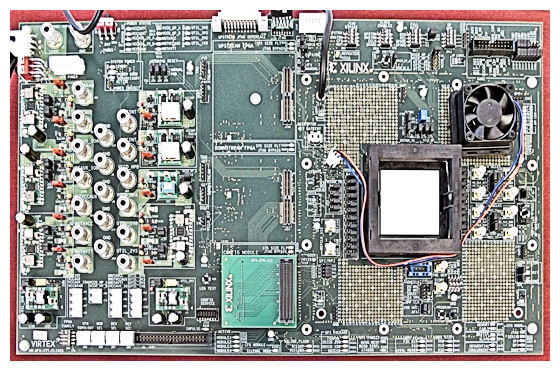
\includegraphics[height=60mm]{Figures/fpga.jpg}

% Title, author and degree
\vspace{0.8cm}
{\FontLb C Compiler for the VERSAT Reconfigurable Processor} \\
\vspace{3.6cm}
{\FontMb Gonçalo da Conceição Reis dos Santos} \\
\vspace{1.9cm}
{\FontLn Thesis to obtain the Master of Science Degree in} \\
\vspace{0.3cm}
{\FontLb Electrical and Computer Engineering} \\
%\vspace{1.9cm}
\vspace{1.0cm}
{\FontSn %
\begin{tabular}{ll}
Supervisor: & Prof. José João Henriques Teixeira de Sousa
\end{tabular} } \\
\vspace{1.0cm}
{\FontMb Examination Committee} \\
\vspace{0.3cm}
{\FontSn %
\begin{tabular}{ll}
Chairperson: & Prof. Francisco André Corrêa Alegria\\
Supervisor: & Prof. José João Henriques Teixeira de Sousa \\
Member of the Committee: & Prof. Paulo Ferreira Godinho Flores \\
\end{tabular} } \\
\vspace{1.5cm}
{\FontMb November 2019} \\
%
\end{center}

\cleardoublepage
 % file "Thesis_FrontCover.tex"

% ----------------------------------------------------------------------
% Dedication page (optional)
% ----------------------------------------------------------------------
%%%%%%%%%%%%%%%%%%%%%%%%%%%%%%%%%%%%%%%%%%%%%%%%%%%%%%%%%%%%%%%%%%%%%%%%
%                                                                      %
%     File: Thesis_Dedication.tex                                      %
%     Tex Master: Thesis.tex                                           %
%                                                                      %
%     Author: Andre C. Marta                                           %
%     Last modified :  2 Jul 2015                                      %
%                                                                      %
%%%%%%%%%%%%%%%%%%%%%%%%%%%%%%%%%%%%%%%%%%%%%%%%%%%%%%%%%%%%%%%%%%%%%%%%

\null\vskip5cm%
\begin{flushright}
     Dedicated to someone special...
\end{flushright}
\vfill\newpage

 % file "Thesis_Dedication.tex"

% ----------------------------------------------------------------------
%  Acknowledgments (optional)
% ----------------------------------------------------------------------
%%%%%%%%%%%%%%%%%%%%%%%%%%%%%%%%%%%%%%%%%%%%%%%%%%%%%%%%%%%%%%%%%%%%%%%%
%                                                                      %
%     File: Thesis_Acknowledgments.tex                                 %
%     Tex Master: Thesis.tex                                           %
%                                                                      %
%     Author: Andre C. Marta                                           %
%     Last modified :  2 Jul 2015                                      %
%                                                                      %
%%%%%%%%%%%%%%%%%%%%%%%%%%%%%%%%%%%%%%%%%%%%%%%%%%%%%%%%%%%%%%%%%%%%%%%%

\section*{\acknowledgments}

% Add entry in the table of contents as section
\addcontentsline{toc}{section}{\acknowledgments}

I want to thank my supervisor, Professor José Teixeira de Sousa, for the 
opportunity to develop this work and for his guidance and support during that process. 
His help was fundamental to overcome the multiple obstacles that I faced during this work.

I also want to acknowledge Professor Horácio Neto for providing a simple Convolutional 
Neural Network application, used as a basis for the application developed for the 
RV32-Versat architecture.

A special acknowledgement goes to my friends, for their continuous support, and Válter,  
that is developing a multi-layer architecture for RV32-Versat. When everything seemed to 
be doomed he always had a miraculous solution.

Finally, I want to express my sincere gratitude to my family for giving me all the 
support and encouragement that I needed throughout my years of study and through the 
process of researching and writing this thesis. They are also part of this work.\\

\textbf{Thank you.}

 % file "Thesis_Acknowledgements.tex"

% ----------------------------------------------------------------------
%  Abstract (both in English and Portuguese)
% ----------------------------------------------------------------------
%%%%%%%%%%%%%%%%%%%%%%%%%%%%%%%%%%%%%%%%%%%%%%%%%%%%%%%%%%%%%%%%%%%%%%%%
%                                                                      %
%     File: Thesis_Resumo.tex                                          %
%     Tex Master: Thesis.tex                                           %
%                                                                      %
%     Author: Carlos A. Rodrigues                                           %
%     Last modified : 21 Jan 2011                                      %
%                                                                      %
%%%%%%%%%%%%%%%%%%%%%%%%%%%%%%%%%%%%%%%%%%%%%%%%%%%%%%%%%%%%%%%%%%%%%%%%

\section*{Resumo}

% Add entry in the table of contents as section
\addcontentsline{toc}{section}{Resumo}

Inserir o resumo em Portugu\^{e}s aqui com o máximo de 250 palavras e acompanhado de 4 a 6 palavras-chave...

\vfill

\textbf{\Large Palavras-chave:} OpenRISC, Sistema em um chip,...

\cleardoublepage

 % file "Thesis_Resumo.tex"
%%%%%%%%%%%%%%%%%%%%%%%%%%%%%%%%%%%%%%%%%%%%%%%%%%%%%%%%%%%%%%%%%%%%%%%%
%                                                                      %
%     File: Thesis_Abstract.tex                                        %
%     Tex Master: Thesis.tex                                           %
%                                                                      %
%     Author: Andre C. Marta                                           %
%     Last modified :  2 Jul 2015                                      %
%                                                                      %
%%%%%%%%%%%%%%%%%%%%%%%%%%%%%%%%%%%%%%%%%%%%%%%%%%%%%%%%%%%%%%%%%%%%%%%%

\section*{Abstract}

% Add entry in the table of contents as section
\addcontentsline{toc}{section}{Abstract}

Versat is a Coarse-Grain Reconfigurable Array architecture (CGRA), which
implements self and partial reconfiguration by using a simple controller
unit. This report studies the current state of the art in HDL and CGRA
simulation, providing a basis to the development of a simulation environment for
Versat. The main objective of this environment is to provide a faster way to
develop and debug software without the use of prototyping hardware. Therefore,
the two types of HDL simulators, event-driven and cycle-accurate, their
advantages and disadvantages are studied, along with a performance comparison
between them. A study of high-level implementations for CGRA simulation is
also presented.

\vfill

\textbf{\Large Keywords:} Versat, coarse-grain reconfigurable arrays, HDL
simulation, CGRA simulation, high-level simulation

 % file "Thesis_Abstract.tex"

% ----------------------------------------------------------------------
%  Table of contents, list of tables, list of figures and nomenclature
% ----------------------------------------------------------------------

% Table of contents
%
\tableofcontents
%\clearpage
\cleardoublepage

% List of tables
%
% Generate list
\listoftables
% Add entry in the table of contents as section
\addcontentsline{toc}{section}{\listtablename}
\cleardoublepage

% List of figures
%
% Generate list
\listoffigures
% Add entry in the table of contents as section
\addcontentsline{toc}{section}{\listfigurename}
\cleardoublepage

% Nomenclature
%
% entries of nomenclature list
%%%%%%%%%%%%%%%%%%%%%%%%%%%%%%%%%%%%%%%%%%%%%%%%%%%%%%%%%%%%%%%%%%%%%%%%%%
%                                                                      %
%     File: Thesis_Nomenclature.tex                                    %
%     Tex Master: Thesis.tex                                           %
%                                                                      %
%     Author: Gonçalo Santos                                           %
%     Last modified : 20 Oct 2018                                      %
%                                                                      %
%%%%%%%%%%%%%%%%%%%%%%%%%%%%%%%%%%%%%%%%%%%%%%%%%%%%%%%%%%%%%%%%%%%%%%%%
%
% The definitions can be placed anywhere in the document body
% and their order is sorted by <symbol> automatically when
% calling makeindex in the makefile
%
% The \glossary command has the following syntax:
%
% \glossary{entry}
%
% The \nomenclature command has the following syntax:
%
% \nomenclature[<prefix>]{<symbol>}{<description>}
%
% where <prefix> is used for fine tuning the sort order,
% <symbol> is the symbol to be described, and <description> is
% the actual description.

% ----------------------------------------------------------------------
% Roman symbols [r]
\nomenclature[ru]{$\bf u$}{Velocity vector.}
\nomenclature[ru]{$u,v,w$}{Velocity Cartesian components.}
\nomenclature[rp]{$p$}{Pressure.}
\nomenclature[rC]{$C_D$}{Coefficient of drag.}
\nomenclature[rC]{$C_L$}{Coefficient of lift.}
\nomenclature[rC]{$C_M$}{Coefficient of moment.}

% ----------------------------------------------------------------------
% Greek symbols [g]
\nomenclature[g]{$\rho$}{Density.}
\nomenclature[g]{$\alpha$}{Angle of attack.}
\nomenclature[g]{$\beta$}{Angle of side-slip.}
\nomenclature[g]{$\mu$}{Molecular viscosity coefficient.}
\nomenclature[g]{$\kappa$}{Thermal conductivity coefficient.}

% ----------------------------------------------------------------------
% Subscripts [s]
\nomenclature[s]{$x,y,z$}{Cartesian components.}
\nomenclature[s]{$i,j,k$}{Computational indexes.}
\nomenclature[s]{$\infty$}{Free-stream condition.}
\nomenclature[s]{ref}{Reference condition.}
\nomenclature[s]{$n$}{Normal component.}

% ----------------------------------------------------------------------
% Supercripts [t]
\nomenclature[t]{T}{Transpose.}
\nomenclature[t]{*}{Adjoint.}

 % file "Thesis_Nomenclature.tex"
%
% Insert glossary/nomenclature section produced by MakeIndex
%%\printnomenclature
% Add entry in the table of contents as section
%%\addcontentsline{toc}{section}{\nomname}
%%\cleardoublepage

% entries of glossary list
%%%%%%%%%%%%%%%%%%%%%%%%%%%%%%%%%%%%%%%%%%%%%%%%%%%%%%%%%%%%%%%%%%%%%%%%%%
%                                                                      %
%     File: Thesis_Glossary.tex                                        %
%     Tex Master: Thesis.tex                                           %
%                                                                      %
%     Author: Carlos A. Rodrigues                                           %
%     Last modified : 30 Oct 2012                                      %
%                                                                      %
%%%%%%%%%%%%%%%%%%%%%%%%%%%%%%%%%%%%%%%%%%%%%%%%%%%%%%%%%%%%%%%%%%%%%%%%
%
% The definitions can be placed anywhere in the document body
% and their order is sorted by <symbol> automatically when
% calling makeindex in the makefile
%
% The \glossary command has the following syntax:
%
% \glossary{entry}
%
% The \nomenclature command has the following syntax:
%
% \nomenclature[<prefix>]{<symbol>}{<description>}
%
% where <prefix> is used for fine tuning the sort order,
% <symbol> is the symbol to be described, and <description> is
% the actual description.

% ----------------------------------------------------------------------

\glossary{name={\textbf{MDO}},description={Multi-Disciplinar Optimization is an engineering technique that uses optimization methods to solve design problems incorporating two or more disciplines.}}

\glossary{name={\textbf{CFD}},description={Computational Fluid Dynamics is a branch of fluid mechanics that uses numerical methods and algorithms to solve problems that involve fluid flows.}}

\glossary{name={\textbf{CSM}},description={Computational Structural Mechanics is a branch of structure mechanics that uses numerical methods and algorithms to perform the analysis of structures and its components.}}

 % file "Thesis_Glossary.tex"

% Insert glossary section produced by MakeIndex
%%\printglossary
% Add entry in the table of contents as section
%%\addcontentsline{toc}{section}{\glossaryname}
%%\cleardoublepage

% Set arabic numbering (1,2,...) after preface
%
\setcounter{page}{1}
\pagenumbering{arabic}

% ----------------------------------------------------------------------
%  Chapters
% ----------------------------------------------------------------------

%%%%%%%%%%%%%%%%%%%%%%%%%%%%%%%%%%%%%%%%%%%%%%%%%%%%%%%%%%%%%%%%%%%%%%%%
%                                                                      %
%     File: Thesis_Introduction.tex                                    %
%     Tex Master: Thesis.tex                                           %
%                                                                      %
%     Author: Andre C. Marta                                           %
%     Last modified :  2 Jul 2015                                      %
%                                                                      %
%%%%%%%%%%%%%%%%%%%%%%%%%%%%%%%%%%%%%%%%%%%%%%%%%%%%%%%%%%%%%%%%%%%%%%%%

\chapter{Introduction}
\label{chapter:introduction}




In this report, the problem of accelerating the execution of Deep Neural
Networks (DNNs) using Coarse GRained Reconfigurable Arrays (CGRAs) is studied,
with special emphasis on compiling a DNN description into code that runs on
CPU/CGRA system. The Deep Versat Architecture~\cite{valter:deepversat} CGRA will be used as an
implementation tool in this work.


%%%%%%%%%%%%%%%%%%%%%%%%%%%%%%%%%%%%%%%%%%%%%%%%%%%%%%%%%%%%%%%%%%%%%%%%
\section{Problem}
\label{section:problem}

Neural Networks have been an object of study since the 1940's, but until the
beginning of this decade their applications were limited and did not play a
major role in computer vision conferences. With its meteoric rise in research,
several solutions to accelerate this algorithm have appeared, from Field Programmable Gate Arrays (FPGA) to
Application Specific Integrated Circuits (ASIC) implementations.

Convolutional Neural Networks (CNNs) are a particular kind of DNN where the output
values of the neurons in one layer are convolved with a kernel to produce the
input values of the neurons of the next layer. This algorithm is compute bound,
that is, its performance depends on how fast it can do certain calculations, and
depend less on the memory access time. Namely the convolutional layers take
approximately 90$\%$ of the computation time.

The acceleration of these workloads is a matter of importance for today's
applications such as image processing for object recognition or simply to
enhance certain images. Other uses like instant translation and virtual
assistants are applications of neural networks and their acceleration is of
vital importance to bring them into Internet of Things.

A suitable circuit to accelerate DNNs in hardware is the CGRA. A CGRA is a
collection of Functional Units and memories with programmable interconnections
in order to form computational datapaths. A CGRA can be implemented in both
FPGAs and ASICs. CGRAs can be reconfigured much faster than FPGAs, as they have
much less configuration bits. If reconfiguration is done at runtime, CGRAs add
temporal scalability to the spacial scalability that characterize
FPGAs. Moreover, partial reconfiguration is much easier to do in CGRAs compared
to FPGAs which further speeds up reconfiguration time. Another advantage of
CGRAs is the fact that they can be programmed entirely in software, contrasting
with the large development time of customized Intellectual Property (IP) blocks.
The Coarse Grain Reconfigurable Arrays (CGRA) is a midway acceleration solution
between FPGAs, which are flexible but large, power hungry and difficult to
reprogram, and ASICs, which are fast but generally not programmable.

However, mapping a specific DNN to a CGRA requires knowledge of its
architecture, latencies and register configurations, which may become a lengthy
process, especially if the user wants to explore the design space for several
DNN configurations. An automatic compiler that can map a standard DNN
description into CPU/CGRA code would dramatically decrease time to market of its
users. Currently there are equivalent tools for CPUs and GPUs and
even for FPGAS.


%%%%%%%%%%%%%%%%%%%%%%%%%%%%%%%%%%%%%%%%%%%%%%%%%%%%%%%%%%%%%%%%%%%%%%%%
\section{Solution}
\label{section:solution}

The proposed solution is a compiler that takes a configuration file from a
neural network framework like Caffe or Darknet. This new tool inputs the
parameters of Deep Versat, such as the number of layers and functional units,
and produces the C code needed for the Versat runs. This code is run on the
RISC-V picorv32~\cite{picorv} CPU controller that has Deep Versat as a peripheral.

%%%%%%%%%%%%%%%%%%%%%%%%%%%%%%%%%%%%%%%%%%%%%%%%%%%%%%%%%%%%%%%%%%%%%%%%
%\section{Thesis Outline}
%\label{section:outline}

%Briefly explain the contents of the different chapters...

%%%%%%%%%%%%%%%%%%%%%%%%%%%%%%%%%%%%%%%%%%%%%%%%%
%\section{Author's Work}
%\label{section:authorwork}

%TO ADD----

%%%%%%%%%%%%%%%%%%%%%%%%%%%%%%%%%%%%%%%%%%%%%%%%%%
\section{Report Outline}
\label{reportoutline}

This report is composed of 4 more chapters. In the second chapter, the
state-of-the-art of neural networks and the difficulties accelerating them is
described. In the third chapter, the Deep Versat architecture and how to program
it is explained. In the fourth chapter, CNN compiler techniques are
explored. Finally, the last chapter contains the proposed solution and the plan
for its execution.



\cleardoublepage

%%%%%%%%%%%%%%%%%%%%%%%%%%%%%%%%%%%%%%%%%%%%%%%%%%%%%%%%%%%%%%%%%%%%%%%%
%                                                                      %
%     File: Thesis_StateOfTheArt.tex                                   %
%     Tex Master: Thesis.tex                                           %
%                                                                      %
%     Author: Gonçalo Santos                                           %
%     Last modified : 20 Oct 2018                                      %
%                                                                      %
%%%%%%%%%%%%%%%%%%%%%%%%%%%%%%%%%%%%%%%%%%%%%%%%%%%%%%%%%%%%%%%%%%%%%%%%

\chapter{State of the Art} % 20
\label{chapter:estadodaarte}

In this chapter a description of the current state of compiler frameworks and
their application to reconfigurable processors is presented. The chapter begins
by explaining the concept of Coarse Grained Reconfigurable Array ({\sc CGRA}), in
order to introduce the Versat reconfigurable processor. Then, several compiler
frameworks are studied with the purpose of selecting a tool for the development
of the Versat compiler. A section about {\sc CGRA} compilers and a comparative
analysis closes the chapter.


\section{CGRA}

A {\sc CGRA} is a programmable hardware structure made of coarse grained
components such as Arithmetic and Logic Units ({\sc ALUs}) whose function (add,
multiply, shift, {\it etc.}) and
interconnection can be programmed differently for
executing different applications~\cite{Tripp07}. {\sc CGRA}s can be controlled by one
or more host processors. By selecting the appropriate components the performance
can optimized, and the total power consumption can be significantly reduced.  The
wiring between the components can then be programmed prior to data
processing~\cite{Cao17TVLSI,Dave18DAC,Gu18TPDS}.  Recent developments allow the
configuration of address generators that implement nested loops in a few
instructions, reducing the configuration time of {\sc CGRA}s~\cite{deSutter10}.
Instead of using a single static configuration for each program, {\sc CGRA}s can
now be reconfigured multiple times during program execution, {\it i.e.} dynamic
reconfiguration~\cite{Hartenstein01}.  However, since reconfiguration consumes
execution time, a balance must be met in order to achieve good
performance~\cite{Mukherjee17VLSID}.

\section{Versat}
\label{section:versat}

{\it Versat} is a {\sc CGRA} architecture where each piece of the program being
executed can use a different composition of functional units~\cite{deSousa12}.
It is used as a hardware accelerator for embedded systems.  It uses a controller
to generate and update the configuration, the {\it picoVersat}.  The controller
is programmable and executes programs written in {\bf C} and assembly (specific
to the architecture).  Contrary to most {\sc CGRA}s, which can only be fully
reconfigured, {\it Versat} allows for partial reconfiguration (where only few
configuration bits are changed), thus optimizing configuration changes.
Moreover, in this approach the configurations are self-generated. Consequently,
the host does not have to manage the reconfiguration process and is free to
perform more useful tasks~\cite{Lopes2017}.  {\it Versat} uses an address
generation scheme that is able to support nested loops expressed in a single
{\sc CGRA} configuration.  Due to the better silicon area utilization and power
efficiency of heterogeneous {\sc CGRA}s architectures, when comparing to
homogeneous ones, an heterogeneous structure was adopted for {\it Versat}.

\subsection{Architecture}

{\it Versat} can be used by host processors in the same chip (allows for
procedures to run faster and with less power consumption), and was designed for
fixed-point signal processing. Its architecture itself is composed of five
different components and is shown in figure~\ref{fig:versat_arch}. These
components are a Controller, a Control Register File ({\sc CRF}), the Data
Engine ({\sc DE}), the Configuration Module ({\sc CM}), and the {\sc DMA}.


\begin{figure}[!htbp]
    \centerline{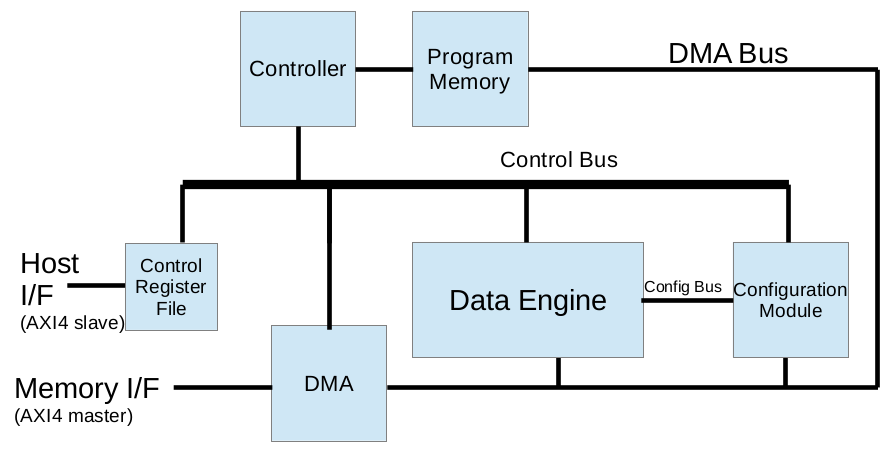
\includegraphics[width=0.8\textwidth]{Figures/top.png}}
    \vspace{0cm}\caption{{\it Versat} top-level architecture.}
    \label{fig:versat_arch}
\end{figure}

The Controller is a programmable component of the architecture that has a direct
dependency with the host that is controlling it, and is in charge of the data
flow, algorithm calculation, and control of the self configuration. The control
data is passed to the other sectors of {\it Versat} through a Control Bus like
for example the attached Serial Divider. The Controller that is used is called
{\it picoVersat}.  The {\sc DE} is the module that does the computations and is
composed of interconnected Functional Units ({\sc FUs}).  The {\sc CM} has the
configurations of the datapaths that are meant to be executed by the {\sc
  DE}. It also allows for partial reconfiguration and for the change of
configuration in runtime.  The {\sc DMA} is a module that works in parallel with
{\it Versat} and has the function of transferring the configurations, programs
and data needed for the execution to and from {\it Versat}.

\subsubsection{Data Engine ({\sc DE})}

The {\sc DE} has a fixed topology comprised of 15 Functional Units ({\sc FUs})
organized in a mesh as shown in figure~\ref{fig:data_engine}.

\begin{figure}[!htbp]
    \centerline{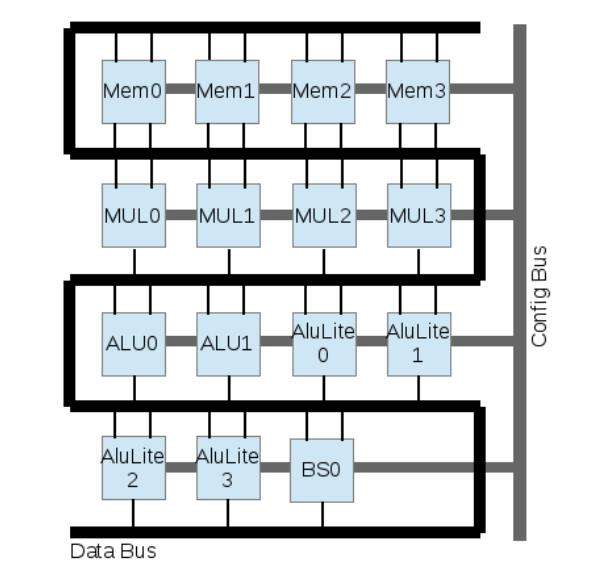
\includegraphics[width=0.7\textwidth]{Figures/DataEngine.jpg}}
    \vspace{0cm}\caption{Data Engine Structure.}
    \label{fig:data_engine}
\end{figure}

The {\sc DE} is a 32-bit architecture containing 15 {\sc FUs} which consist of
one barrel shifter, six {\sc ALUs}, four multipliers and four dual-port 8kB
embedded memories.  The system's Controller reads and writes from the {\sc FUs}
and to the memories.

Each {\sc FU} reads it's configuration of an operation and an input selection
from the Configuration Bus.  All {\sc FUs} write their 32 bit output to a wide
Data Bus of 19x32 bits.  The operations are chosen from a fixed number of those
that are available to the accelerator.

The {\sc DE} can be configured using one or more hardware datapaths, which
allows for Data Level Parallelism ({\sc DLP}) or Instruction level Parallelism
({\sc ILP}) depending on if the execution happens in parallel lanes or if the
paths are pipelined, respectively. Datapaths can operate in parallel in this
architecture as long as the resources needed to execute each of the datapaths are
available, which also gives {\it Versat} the capability of having Thread Level
Parallelism ({\sc TLP}).

Some of the most used cases of parallelism can be described by the following
examples of hardware datapaths.  In figure~\ref{fig:de_datapaths} there are
shown three examples of datapaths describing these cases of parallelism.

\begin{figure}[!htbp]
    \centerline{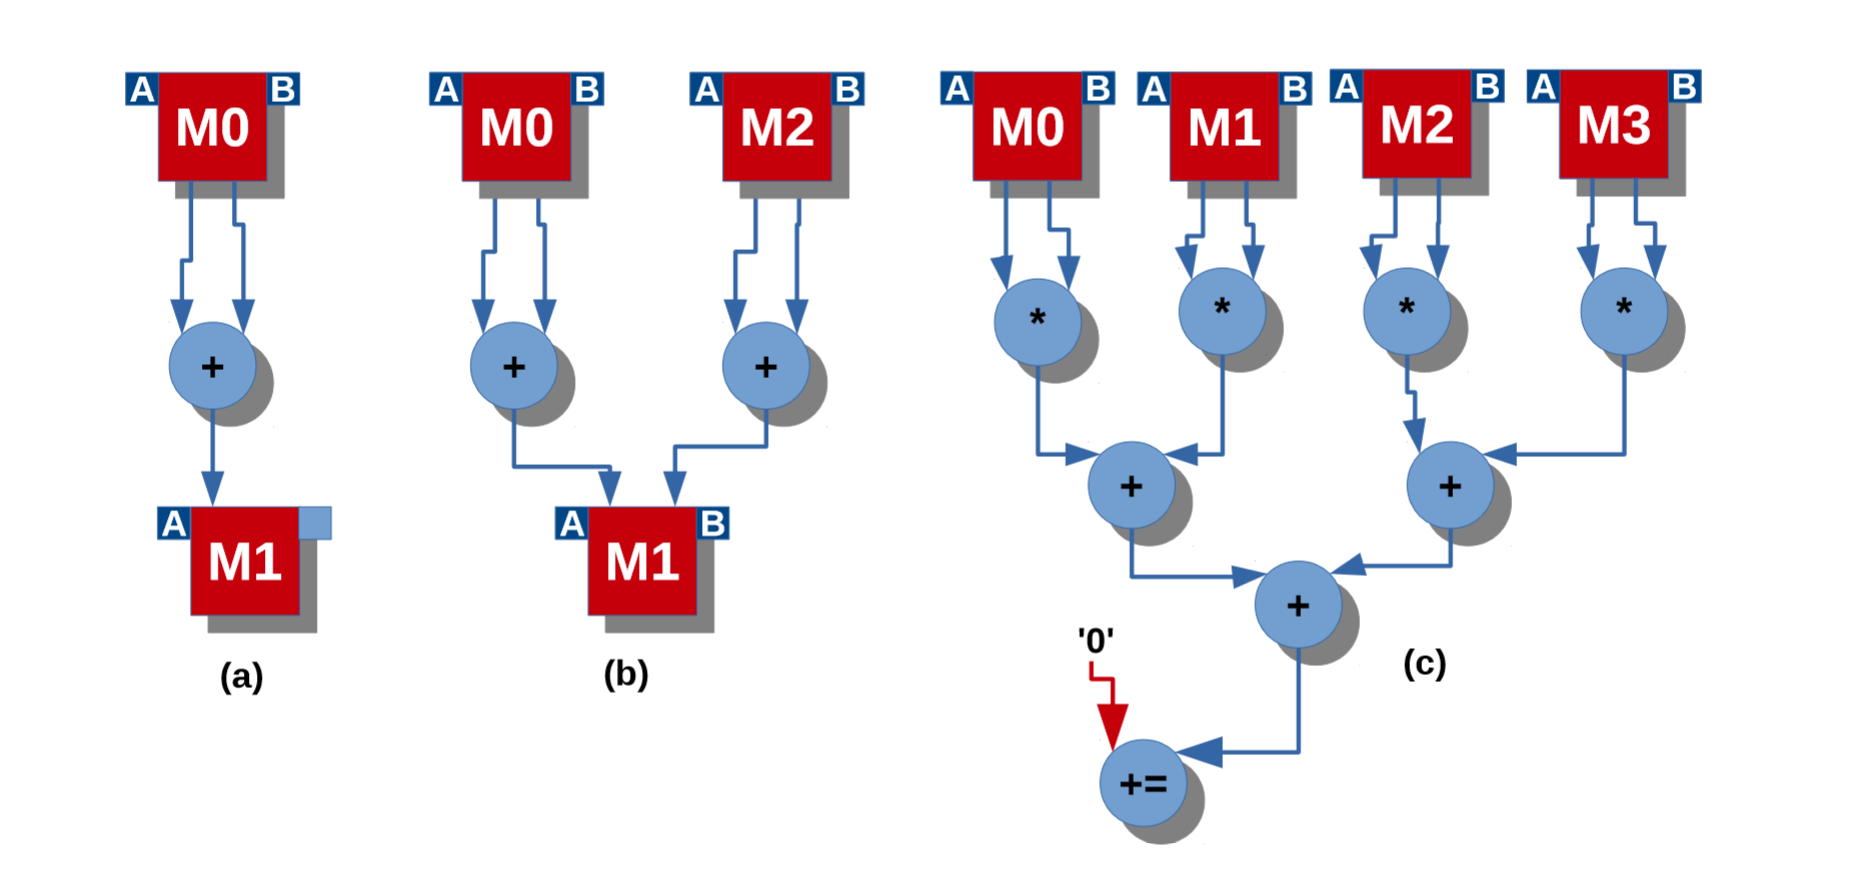
\includegraphics[width=0.8\textwidth]{Figures/de_datapaths.png}}
		\vspace{0cm}\caption{Data Engine Structure configuration examples with dual-port
		(A and B), memories (M0 to M3), and functional units (adders and multipliers).}
    \label{fig:de_datapaths}
\end{figure}

Because of the nature of the architecture, pipelined vector addition, the memory
read and write operation, and the addition operation, can be done in parallel, for
consecutive elements of that vector, as shown in (a).  It is possible to do
multiple pipelined vector addition operation using data from different memories
and saving the results in the same or different memories in parallel, if the
data itself is not dependent on each other, like in the case of (b).  When there
is a need to do the inner product of two vectors, since in this case elements
from each vector are multiplied, then the results are added and accumulated,
which is shown in datapath (c).  All of the {\sc ALU} operations described can
be executed in parallel~\cite{Lopes2017}.

There is an independent Address Generation Unit ({\sc AGU}) for each port of the
memories used, which allow for two level nested loops, and execution start with
a programmable delay.  {\sc TLP} can be exploited because the {\sc AGUs} can
operate independently, making it possible, for example, to operate through data
in different memories using two threads and then save the values obtained in the
same goal memory.
% explicar mais AGUs se for necessario

\subsubsection{Configuration Module}

The Configuration Module ({\sc CM}) is composed of three elements which are the
Configuration Register File ({\sc CRF}), the Configuration Shadow Register ({\sc
  CSR}) and the Configuration Memory ({\sc CM}), as shown in
figure~\ref{fig:config_module}.

\begin{figure}[!htbp]
    \centerline{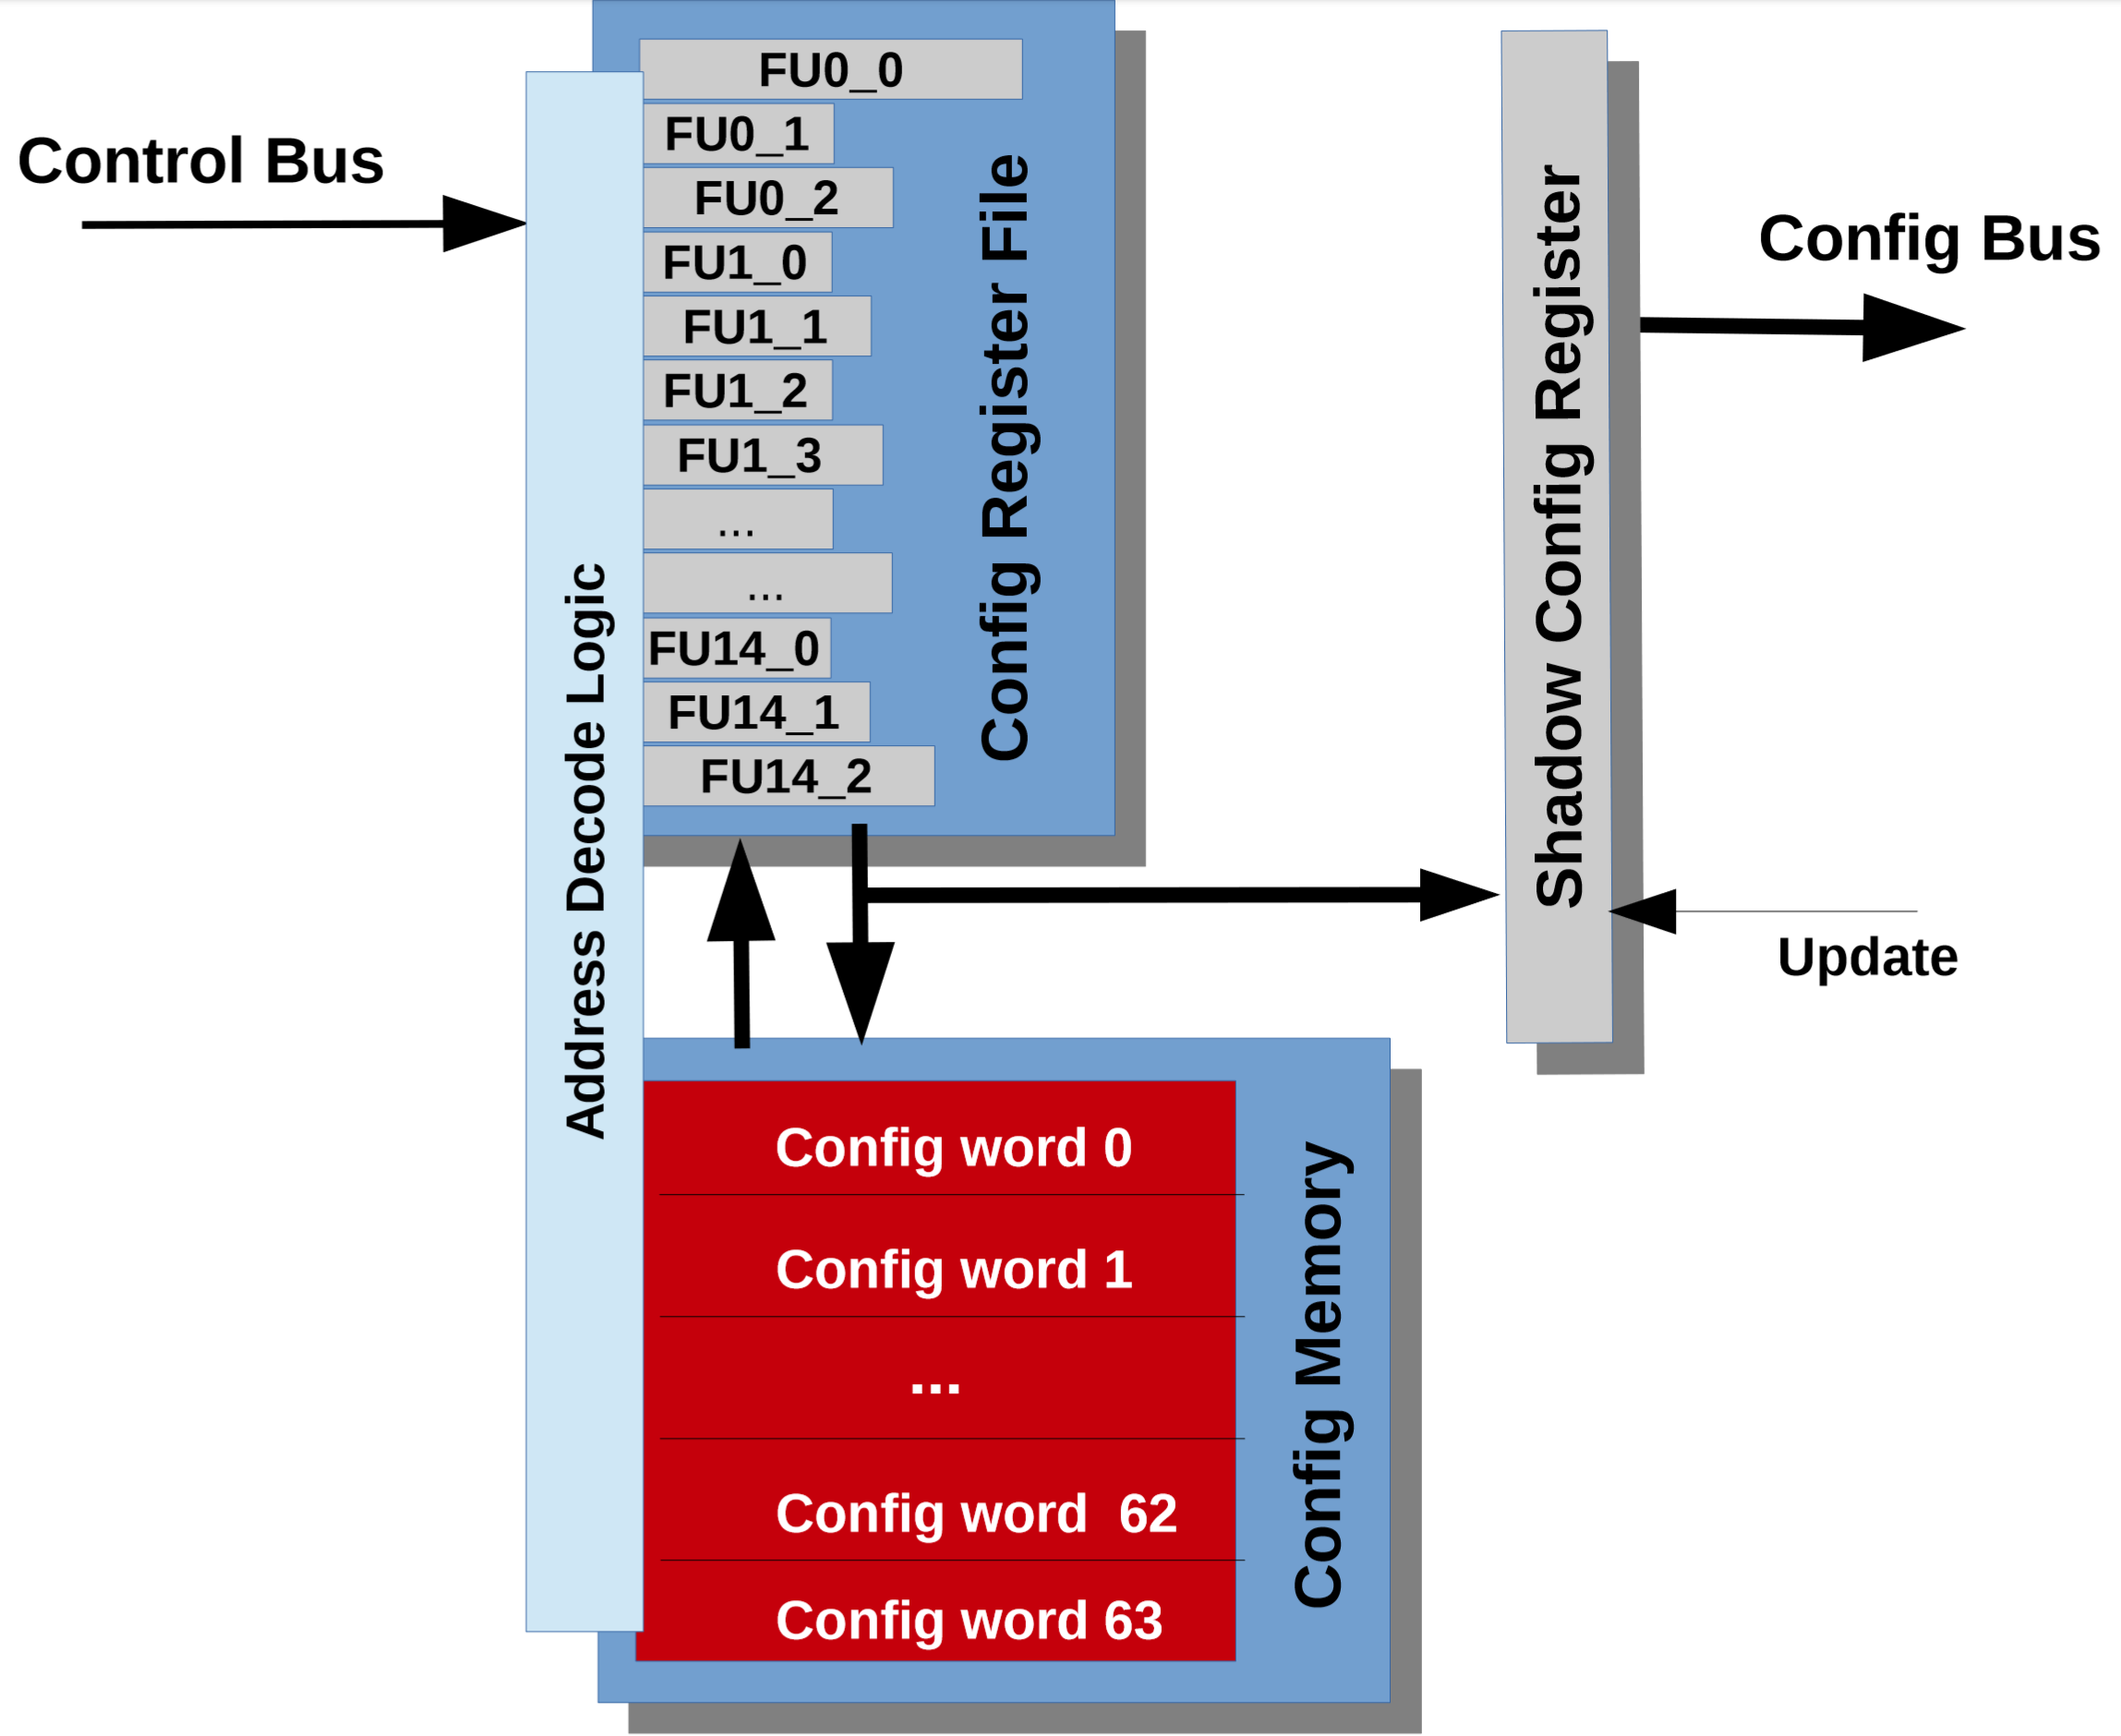
\includegraphics[width=0.7\textwidth]{Figures/config_module.png}}
    \vspace{0cm}\caption{Configuration Module Structure.}
    \label{fig:config_module}
\end{figure}

The preparation of the next configuration to be executed by the {\sc DE} is done
by the {\sc CRF}. It is an element composed of 118 configuration fields, and each
of these differ on the number of bits they define, totaling a full configuration
of 672 bits. By having each of these fields separate, it is possible to take
advantage of the fact that, during the execution of most of the application
code, there is a high chance that the {\sc DE} configurations used are very
similar to each other.  A partial reconfiguration can be done more effectively
since they differ in a low number of fields.

During execution, the current {\sc DE} configuration is present in the {\sc
  CSR}. This configuration is updated by copying the configuration in the {\sc
  CRF} to the {\sc CRS} when an {\it Update Signal} is sent by the
Controller. This allows for the reconfiguration of the system using the {\sc
  CRF} while the configuration in the {\sc CSR} is running (hidden
reconfiguration in runtime).

Because some {\sc DE} configurations are very common there is a dedicated memory
for the most common configurations. Each configuration has 672 bits this
in a dual-port 64 position memory. The configurations saved in this memory can
be loaded/stored from/to the {\sc CRF} in a single clock cycle through one of
the memory ports while the other port is 32-bits wide and is used to load/store
in an external memory by using the {\sc DMA}, so that the {\sc CM} is able to
exceed 64 positions.

\subsubsection{Controller} % 5
\label{section:picoversat}

{\it picoVersat} is a minimal hardware controller with a reduced instruction set
and few registers, with the purpose of doing simple calculations and giving
instructions to its connected systems. Therefore this controller is not designed
for high performance computation, even if it is able to effectively implement
simple algorithms.  It is a programmable solution which mitigates the risk of
hardware design mistakes, and helps the design and implementation of more
complex control structures.  This controller is simple and has a reduced silicon
area which allows for a low power consumption.

\subsection{picoVersat (Controller)}
The controller's architecture can be represented by the block diagram shown in
figure~\ref{fig:bd}.

\begin{figure}[!htbp]
    \centerline{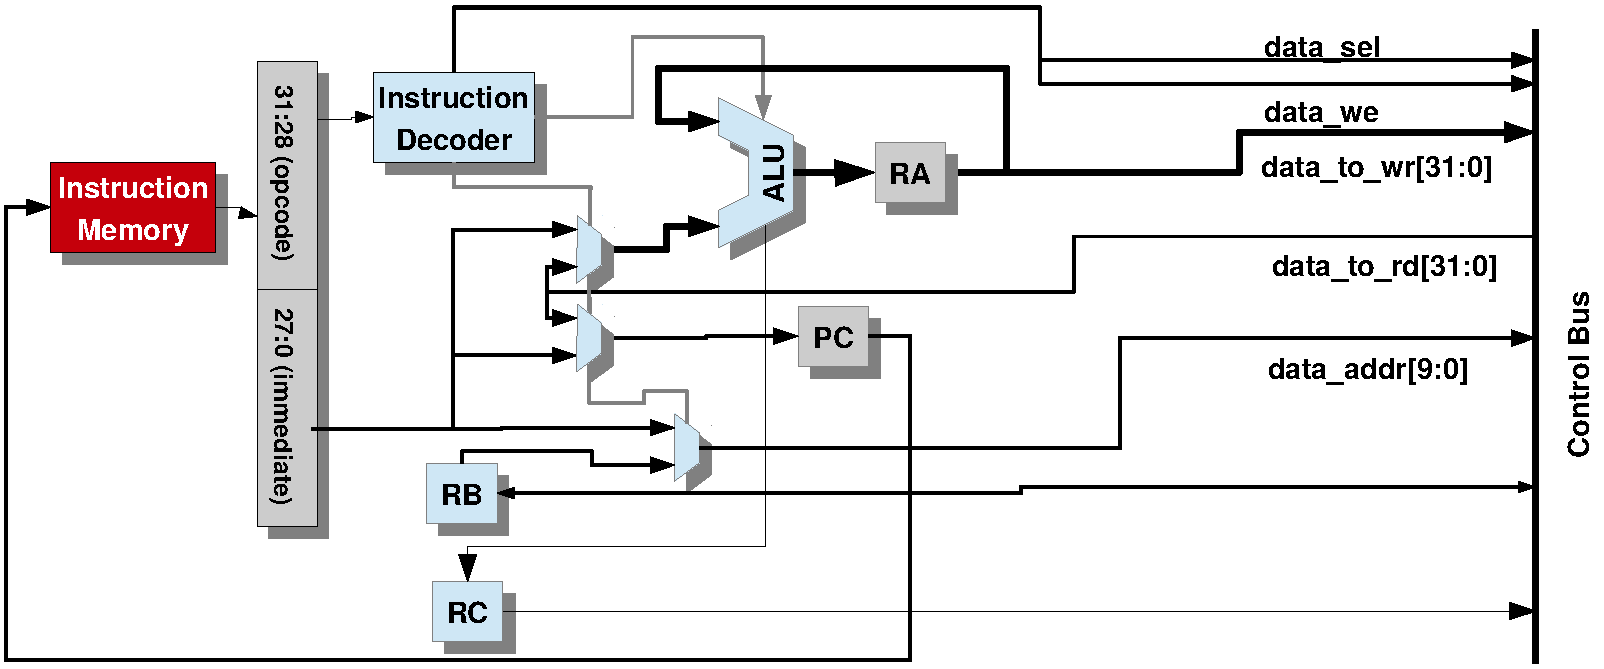
\includegraphics[width=0.9\textwidth]{Figures/bd.pdf}}
		\vspace{0cm}\caption{picoVersat Block Diagram: with registers
		(RA, RB, RC and PC), their interconnections and memory access.}
    \label{fig:bd}
\end{figure}

{\it picoVersat} is composed of four main registers:
\begin{itemize}
\item Register {\bf RA} is the accumulator and is the most relevant of the registers
in the architecture.  It can be loaded with a value read from the data interface
or with an immediate value from an instruction.  It gets the value from the
result of the operations, and is used as an operand itself along with an
immediate value or an addressed value. The value of {\bf RA} is sent to the data
interface.
%
\item Register {\bf RB}, the data pointer, is used to implement indirect loads/stores
to/from the accumulator.  This register is mapped in memory which means it is
accessed by reading/writing as if accessing the data interface.
%
\item Register {\bf RC} is the flag register, storing three operation flags which are
the negative, overflow, and carry flags.  Much like register {\bf RB}, this
register is also memory mapped but this one is mapped to a {\it read only}
section, being only set by the {\sc ALU}.  The structure used for this register
is depicted in Table~\ref{tab:flags}.  As it is shown in Table~\ref{tab:flags} some bits
are not used and could be used to implement other flags but, as of right now,
there has not been a need to add any more.

\begin{table}[!htbp]
  \centering
    \begin{tabular}{|c|c|p{7cm}|}
    \hline
    {\bf Bits} & {\bf Name} & {\bf Description} \\
    \hline \hline
     31-3 & NA & Reserved for future use\\
    \hline
     2 & Negative & Asserted if last {\sc ALU} operation generated a negative result\\
    \hline
     1 & Overflow &  Asserted if last {\sc ALU} operation generated an arithmetic overflow\\
    \hline
     0 & Carry & Asserted if last {\sc ALU} operation generated a carry\\
    \hline

    \end{tabular}
  \caption{Register C: flags}
  \label{tab:flags}
\end{table}

\item The Program Counter, {\bf PC} register, contains the next instruction to be
fetched from the Program Memory so that it can be executed.  This register
increments for every instruction, in order to fetch the next instruction except
for branch, in which the {\bf PC} register is loaded either with an immediate
present in the branch instruction, or with the value present in {\bf RB}.  These
two types of branches implement direct and indirect branches, respectively.
\end{itemize}

For increasing the frequency, by reducing the critical path, the controller
takes two clock cycles to fetch one instruction, in pipeline.  It executes every
instruction that is fetched.  In other words, it has 2 delay slots in the case
of a branch instruction.  These delay slots can be filled with a no-operation
instruction ({\sc NOP}), but the compiler/programmer can also use them to
execute useful instructions.  For instance, in the case of a {\tt for}
loop, the delay slots can be used to write the iteration count to some
register~\cite{Lopes2017}.

\subsubsection{Instruction Set}

The instruction set that is used to run {\it picoVersat} is minimalist and
has only one type.  This type has 32 bits and is divided between an
{\it opcode} and an immediate constant, like it is shown in Table~\ref{tab:if}.

\begin{table}[!htbp]
  \centering
    \begin{tabular}{|c|p{7cm}|}
    \hline
    {\bf Bits} & {\bf Description} \\
    \hline \hline
     31-28 & Operation code (opcode)\\
    \hline
     27-0 & Immediate constant \\
    \hline

    \end{tabular}
  \caption{Instruction format.}
  \label{tab:if}
\end{table}

The operations that the controller can perform are listed in
Table~\ref{tab:isa}.  The notation used for the logic, that represents the
operations, is written with {\bf C} language syntax in mind.
It is also notable that {\it Imm} represents an immediate constant and that
{\it M$[$Imm$]$} represents the contents in address {\it Imm} in memory.

\begin{table}[!htbp]
  \centering
    \begin{tabular}{|c|c|p{8cm}|}
    \hline
    {\bf Mnemonic} & {\bf Opcode} & {\bf Description} \\
    \hline \hline
\multicolumn{3}{|c|}{{\bf Arithmetic / Logic}}\\
\hline \hline
    addi  & 0x0 & RA = RA + Imm; PC=PC+1\\
    \hline
    add   & 0x1 & RA = RA + M[Imm]; PC=PC+1\\
    \hline
    sub   & 0x2 & RA = RA - M[Imm]; PC=PC+1\\
    \hline
    shft  & 0x3 & RA = (Imm $<$ 0) ? RA $<<$ 1: RA $>>$ 1; PC=PC+1\\
    \hline
    and   & 0x4 & RA = RA \& M[Imm]; PC=PC+1\\
    \hline
    xor   & 0x5 & RA = RA $\oplus$ M[Imm]; PC=PC+1\\
    \hline
\multicolumn{3}{|c|}{{\bf Load / Store}}\\
\hline \hline
    ldi   & 0x6 & RA = Imm; PC=PC+1\\
    \hline
    ldih  & 0x7 & RA[31:16] = Imm; PC=PC+1\\
    \hline
    rdw   & 0x8 & RA = M[Imm]; PC = PC+1\\
    \hline
    wrw   & 0x9 & M[Imm] = RA; PC = PC+1\\
    \hline
    rdwb  & 0xA & RA = M[RB+Imm]; PC = PC+1\\
    \hline
    wrwb  & 0xB & M[RB+Imm] = RA; PC = PC+1\\
    \hline
\multicolumn{3}{|c|}{{\bf Branch}}\\
\hline \hline
    beqi  & 0xC & RA == 0 ? PC = Imm: PC += 1; RA = RA-1\\
    \hline
    beq   & 0xD & RA == 0 ? PC = M[RB]: PC += 1; RA = RA-1\\
    \hline
    bneqi & 0xE & RA != 0 ? PC = Imm: PC += 1; RA = RA-1\\
    \hline
    bneq  & 0xF & RA != 0 ? PC = M[RB]: PC += 1; RA = RA-1\\
    \hline

    \end{tabular}
  \caption{Instruction set.}
  \label{tab:isa}
\end{table}

Additionally, the pseudo instruction {\tt nop} can be used
in assembly and is converted by the assembler.
It means No-OPeration or do nothing and is coded as {\tt addi 0}.
The instruction following a branch instruction is always executed due
to the instruction pipeline latency (delayed branch or slot).  Pad with
{\tt nop}s if no useful instructions can be executed.

This controller has the capability to work on its own, that is, the controller
can run the functions and operations that do not depend on the {\it Versat}
accelerator itself without it being connected, which allows the execution of
simple applications that do not have tight time constrains.

\subsection{Previous Compiler}

The previous compiler~\cite{Santiago2017} was made from scratch and
was based around object oriented programming languages like {\it JAVA}
and {\it C++}.  Although, it claims to be
a {\bf C++} dialect, it provides no classes, not even {\bf C} structures,
variables or declarations, and no object-oriented capabilities like
encapsulation or polymorphism.  The use of a `dot' to access object functions
({\em obj.func()}) of predefined objects extends the use of {\bf C} alike
structure addressing to a small set of compiler static dependent objects.

The compiler was developed around the idea that each component of {\it Versat}
is viewed as an object. Each function that each object can perform is called by
referencing the function within the object.  The programming is performed by
calling operations on those predefined objects.  This was a good idea but, since
a true object oriented approach is far too complex for the architecture of a
{\sc CGRA}, the result ended up looking like an object based language but not
working like one.  Instead of using a classic approach where an abstract syntax tree ({\sc AST}) is
built from syntactic description, the compiler only uses components to represent
the {\bf Versat} hardware components.


Before developing the previous compiler existing common compilers were
investigated, like {\bf gcc} or {\bf llvm}, but it was ``concluded that
these compilers are good at producing sequences of instructions but not
sequences of hardware datapaths''~\cite[p.~21]{Lopes2017}.

% these do João lopes, p.21

%Another problem this compiler has is the fact that it does not allow for the coding of some functionalities that the CGRA itself has, as well as not have an implemented optimization step in the {\it back-end} of the compilation process.
% 40KB 10.8Kl 300KB asm, with -S
Another drawback is that this compiler does not allow for the coding of some
functionalities that the {\sc CGRA} itself has, and do not have an implemented
optimization step in the {\it back-end} of the compilation process.
% 40KB 10.8Kl 300KB asm, with -S


The above problems and the aims described in the Objectives section is the
reason why the previous compiler needs to be improved, as is the purpose of this
work.  In order to achieve the objectives there were two options: continue
evolving the previous compiler by adding new functionalities, or to create a new
compiler through a different method that would be more adapted to the type of
architecture.

The first option, even though it seems to be the easiest, suffers from the
problem that it took as a base an object oriented architecture but does not work
like one. To circumvent the previous approach as well as the other problems
described earlier, a research was made in order to see if the other option was
better or worst.

The main advantage of the second option of creating a compiler not from scratch
is that it allows for the user code to be written exactly in the {\bf C}
programming language.
This is a very good advantage, not only because of the extra help given to the
programmer, but also because it would allow to make the optimization simpler.
%, since C code is researched and easier to code than.
Another good point to defend this approach is that the controller itself can
work on it's own, without the {\it Versat} accelerator, being able to run any
{\bf C} code, even if much slower that with the accelerator connected.

\section{Compilers} % 7
\label{section:compilers}
%escolha do compilador mais detalhada no final (seccao seguinte)


Since using the previous compiler as a starting point is not a good option,
existing compilers should be investigated.  First, the components of a compiler
must be analyzed.  Then, taking into account the usage of compiler components by
existing compilers, a selection of widespread compilers is analyzed.  Finally, a
comparative analysis of the most common compilers is performed in order to
select candidates suitable for conversion.  The converted compiler should
generate {\em picoVersat} assembly, identify and configure the {\em Versat} {\sc
  CGRA} architecture.

Computer programming, and processor programming in particular, is a complex and
time consuming task.  Computers execute binary code, but writing binary code is
an error prone and meticulous task reserved for very small low level
programming.  Assembly provided a textual approach to computer programming,
while keeping full control over the instruction set for a particular processor.

A compiler is a tool that allows the programmer to write abstract high-level
instructions and produces assembly code for the processor~\cite{aho06,cooper03}.
The assembler tool can then be used to transform the assembly instructions into
binary instructions of the processor.  The compiler can also perform semantic
error detection and data flow analysis, thus improving the required development
cycle and the generated code quality.  A good compiler can produce optimized
code as good, or sometimes better, than the manually written assembly
equivalent.

In order to transform a high-level programming language into assembly code, the
compiler tool is composed of two major phases: an analysis phase and a synthesis
phase.  During the analysis phase the input file is read, byte by byte, and
structured into an abstract syntax tree ({\sc AST}) containing all the relevant
information for final code generation.  The synthesis phase transforms an {\sc
  AST} into machine code assembly instructions~\cite{cooper03,appel08}.  These phases
correspond to, what is called in compiler terminology, the {\it front-end} and the
{\it back-end}, respectively.

%chap 1.2, 1.3

\subsection{Analysis}

The analysis phase is decomposed into three analysis stages: lexical,
syntactical and semantic.  The stages are pipelined in such a way that the
output of a lexical analyzer is fed into a syntactic analyzer, and the output of
the syntactic analyzer is coupled with the semantic analyzer.  At the end of the
syntactic analysis, the language in the input file is converted into an {\sc
  AST}.

\subsubsection{Lexical analysis}\label{lex}

The lexical analysis processes the input file, containing the high-level
computer program, into identifiable {\em tokens}~\cite{schreiner85,lexyacc95}.
The {\em tokens} are symbols or words that play a specific role in the input
language.  For instance, in the {\bf C} programming language, braces and
semi-columns, among others, are of particular interest~\cite{cpl}.  Other {\em
  tokens} may include identifiers, operators and language reserved keywords such
as data types or flow control.  The lexical analysis also removes information
that is irrelevant for code compilation, including comments and white-spaces.

The lexical analysis can be performed using simple and efficient algorithms
based on regular expressions.  However, as it is tedious, difficult to amend and
error prone work, lexical generator can be used to automate and simplify the
lexical generator.  The lexical analyzer generator {\bf lex}~\cite{Lesk:lex} and
its successors, like {\bf flex} or {\bf jflex}, can produce very compact and
efficient lexical analyzers from a simple description based on regular
expressions and embedded {\bf C} or {\bf C++} code.

\subsubsection{Syntactic analysis}\label{yacc}

The syntactic analysis phase structures a sequence of {\em tokens} provided by
lexical analysis into a tree of tokens~\cite{schreiner85,lexyacc95}.  The
purpose of the syntactic analysis is to check the order of the {\em tokens} and
identify the language constructs that they aim to describe.  After the syntactic
analysis the structure of the program is well defined and constructs like
expressions, instructions, functions and variable declarations have been
identified.

The syntactic analysis, as the lexical analysis, can be greatly simplified using
efficient algorithms.  However, these algorithms are more complex and time
consuming than the ones used in the lexical analysis.  These algorithms are
grouped into two different groups, {\bf LL} and {\bf LR}, depending whether the
constructs are identified {\bf L}eft-to-right or {\bf R}ight-to-left (the second
letter in the acronym, since the first reveals the {\em token} arriving order
which is always {\bf L}eft-to-right).  The syntactic analysis is described by a
context-free grammar describing the constructs of the high-level language being
processed.  Depending on the specific algorithm used to parse the grammar, a
different but equivalent grammar must be found.  The {\bf LALR(1)} algorithm,
which stands for {\bf L}ook-{\bf A}head {\bf LR} with a single lookahead {\em
  token}, allows a wide range of equivalent grammars, making the discovery of a
suitable grammar for the high-level language a simple task.

As for the lexical analysis, also the syntactic analyzer can be generated using
an automated tool from a grammar description with {\bf C} or {\bf C++} code
insert using tools like {\bf yacc}~\cite{Johnson:yacc} or {\bf
  bison}~\cite{donnelly03}.  The code insert are used to build the {\bf AST}.
Frequently, each grammar rule produces a tree node in the {\sc AST}.
Tools like {\bf antlr}, a {\bf SLL(*)} (a {\bf S}trong {\bf LL} with
arbitrary lookahead {\bf (*)} parser generator), provide mechanisms to
automate the construction of the {\sc AST}~\cite{parr07}.

\subsubsection{Semantic analysis}

The semantic analysis phase is responsible for checking if the constructs,
identified by the syntactic grammar, are accepted by the high-level language
and can be performed by the computer.  It must check if a variable was already
declared or if the operation request can be performed by the variable.  The
semantic analysis results from the fact that grammar must be context-free in
order to be processed by efficient syntactic algorithms.

The semantic analyzer scans the {\bf AST} for inconsistencies and prevents code
from being generated for erroneous programs.  Since semantic check is very
dependent on the high-level language particulars, it is usually performed by the
host language ({\bf C} or {\bf C++} in most cases) after, or even during, the
syntactic analysis.
%chap 8.1.1 - 8.1.5, 8.2.1 - 8.2.6

\subsection{Synthesis}

The synthesis phase is no longer dependent on the input high-level language.
Many compilers produce the {\sc AST} from different high-level languages,
although some languages may not generate some type of nodes.  On the other hand,
many compilers produce code for different processors and computer architectures
from the same {\bf AST}~\cite{hanson95}.

The synthesis phase is comprised of several stages: instruction selection,
instruction scheduling, register allocation, optimization, and data flow
analysis.  Code synthesis is an NP-complete problem and a particular order of
stages does not necessarily produce the best code, since a good decision in one
stage can compromise the quality of subsequent stages.  Some compilers repeat
some stages or try different approaches in order to find the best among them.

%chap 13.1, 13.2, 14 (14.1) - explicar cada um

\subsubsection{Instruction selection and scheduling}\label{burg}

Most compilers begin the synthesis phase by the instruction selection.
Instruction selection aims at finding the best processor instructions for a part
of an {\sc AST}~\cite{cooper03,Fraser:burg,Proebsting:2002}.  For instance, an
{\bf arm} processor offers a free sum ({\tt add}) for each multiplication ({\tt
  mul}) and free shift for most arithmetic instructions.  When these pairs of
instructions are found in contiguous tree nodes, a single instruction can be
produced, otherwise each node produces a processor instruction.
%More complex instructions, such as {\em load-effective-address} ({\tt lea}) in {\tt Intel-x86} processors,
An instruction selector generator is a tool based on a grammar that describes
the tree pattern that matches a given processor instruction.  In fact, the
grammar describes the target processor capabilities in terms of tree patterns.
To each tree pattern can be assigned a cost, that measures the time consumed by
the instruction execution.  The selector generator chooses
the best combination of instructions that map all the {\sc AST}, that is where
total cost is minimum.  As a result, the instruction selection produces a
sequence of target processor instructions.  The arguments of the instruction,
that is its registers, are not yet assigned.
Instruction selection can be performed by dynamic programming where the {\sc AST}
is searched twice, one for determining the instruction costs and a second to generate
the best selected instructions.
Therefor, the algorithm is linear on the number of instructions (O(N)).
The instruction selection tools, known as {\sc BURG} ({\bf B}ottom {\bf U}p
{\bf R}ewrite {\bf G}rammar), like {\tt lburg}, {\tt iburg}, {\tt monoburg}
automate the code generation process.

%This step has linear complexity (O(N)) as do most of the algorithms used in compiler development.

\paragraph{{\sc C3E} versus {\sc SSA}}

When representing abstract processor instructions there are two representations:
{\em three address instructions} ({\sc C3E}) and {\em static single assignment}
({\sc SSA})~\cite{appel08,parsons92}.
In {\sc C3E} each instruction takes up to three arguments, one of
them being the destination of the operation.  These instructions arguments are
not yet registers, since register allocation was not performed, but names of
high-level variables.  More recently, since {\sc gcc-4} and in other modern
compilers, the {\sc SSA} has been adopted because it provides a better base for
optimization, allocation and scheduling.  In {\sc SSA} each argument is tagged
with a version number and, each time the variable is reassigned, the version
number is incremented.  Therefor, two registers can contain different versions
of the same variable, allowing for a better use of common sub-expressions.
For instance, in {\tt while (*s++)} both $s_0$ and $s_1$ from $s_1 = s_0 + 1$, the old value is kept in a register for the evaluation of the condition while the new value is stored in memory.

\paragraph{Basic blocks}

A basic block is a sequence of instructions that have no labels between them,
allowing transfer of control into the block, nor have jump instructions among
them.  A jump instruction always ends a basic block.  A label always breaks a
block in two basic blocks.  Within a basic block the sequence of instructions
can be changed, as long as the argument dependencies are kept.


\paragraph{Instruction scheduling}

The scheduling is performed on code basic blocks.  The scheduling rearranges the
order of the instructions taking into account the number of available functional
units in the processor and the latency of their executions.  To each instruction
is given an available functional unit, and a simulation of the execution is
performed to determine when the functional unit is again available for the next
instruction.  For instance, when a multiplication is being performed, other
operations like sums and shifts can be done in parallel as long as there is no
dependency on the arguments.  The rearrangement of the instructions produces the
minimum sum of elapsed time, including latencies.
List scheduling is a greedy heuristic approach that performs a simulation of the
execution of a basic block instructions once (O(N)), but it is quadratic on the
number of operands (O($m^2$)), although for most operations $m$ is one or
two~\cite[p.605]{cooper03}.
For instance, when an operation requires arguments that result from a $sum$ and a $multiplication$, the $multiplication$ is performed first since it has higher latency, and the $sum$ is executed while the $multiplication$ is being performed if both operations can be paralelized.

\subsubsection{Register allocation}

Register allocation aims at finding the best use of the available machine
registers.  On machines with a small number of registers, the process is simple
since there are not that many options.  Modern {\sc RISC} machines register 
allocation, with 16 or more general purpose registers,  is both complex and central
to the efficiency of the resulting code.  Register allocation algorithms are
divided in local, within basic blocks, and global, when involving more than one
basic block.

When performing local register allocation the available registers can be freely
assigned and an optimal algorithm exist, for instance when generating code for
expressions.  Global register allocation usually sets aside some of the
registers and tries to distribute their use among the basic blocks, taking into
account their dependencies (see~Optimization and data flow analysis).
When one basic block uses more
registers, another must be sacrificed, and no optimal solutions exist.  However,
if instructions are limited to {\bf if}, {\bf do}, {\bf while} and {\bf for}
without the indiscriminate use of {\bf goto}, a good solution can be obtained.

Register allocation is based on {\tt live} or {\tt dirty} registers, those that
presently contain a useful value, and {\tt dead} or {\tt clean} registers,
those that can be assigned to new uses.
However, {\tt live} registers can contain a copy of
memory value, allowing for its use without saving, or computed values that must
first be saved before the register can be used for another purpose.  It is up to
the allocation algorithm to find the best combination of registers in order to
reduce the number of memory {\tt loads} and {\tt stores}.

Register allocation algorithms include local algorithms like {\em Sethi-Ullman}
(optimal for expressions), {\em greedy}, {\em next-use} and {\em top-down} or
{\em bottom-up} approaches.  Global allocation uses {\em linear scan} for simple
{\tt just-in-time} compilers and more complex {\em graph coloring} for optimizing
compilers.

\subsubsection{Optimization and data flow analysis} \label{dataflow}

Once the code is generated it can be rearranged.  In fact, optimization begins
with instruction selection and is present in each stage of the synthesis
phase~\cite{allen01,muchnick97}.
Simple optimizations, like {\em peephole} where a sliding window analyses
sequences of adjacent instructions, can be performed after instruction
selection when two nodes produce contiguous instructions that can be
replaced by a better one.
Data flow analysis is an optimization that searches for the best
sequencing of basic blocks, reducing the number of inter-block jumps.  Complex
compilers may provide thousands of optimizations that must be tested in order to
find out if an improvement can be achieved.

\subsection{B language compiler}

The {\bf B} programming language is the predecessor of the {\bf C} programming
language and provides a very similar syntax~\cite{lang:b}.  {\bf B} uses only an
integer data type, eliminating the need for data structures.  It provides access
to single byte characters through literals and library manipulation
routines~(see Figure~\ref{fig:blc}).  All {\bf C} operators and instructions are
present but lacks the {\bf for} construct.  Missing is also the preprocessor.

\begin{figure}[!htbp]
    \centerline{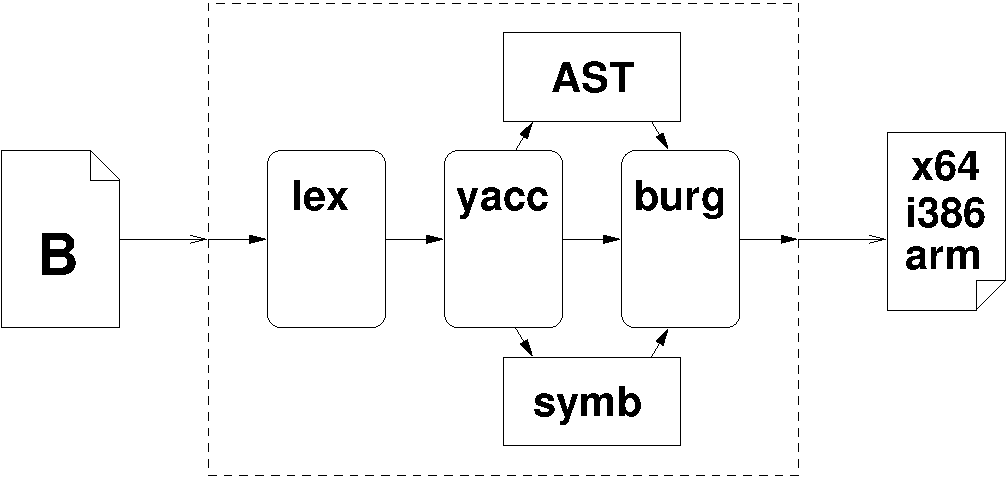
\includegraphics[height=50mm]{Figures/blc.pdf}}
    \vspace{0cm}\caption{{\bf B} language compiler.}
    \label{fig:blc}
\end{figure}

%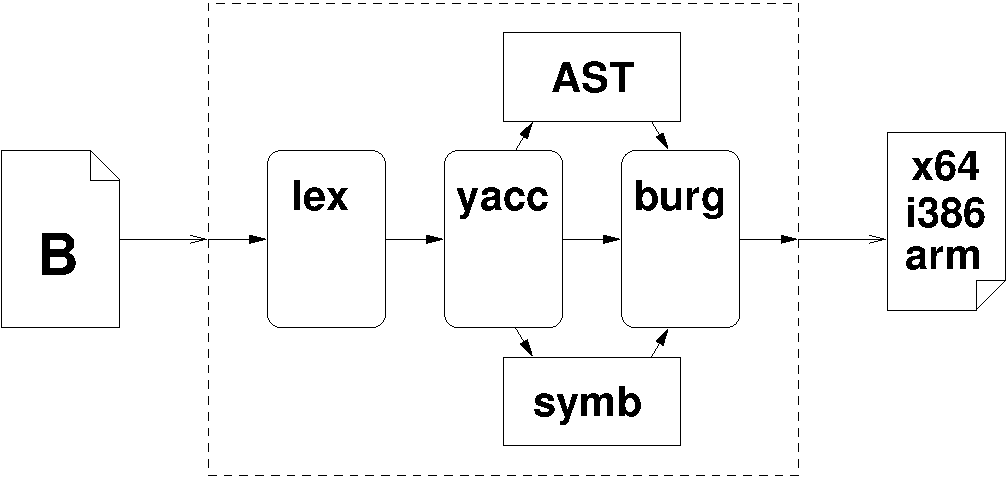
\includegraphics[height=50mm]{Figures/blc.pdf}

The  {\bf B} language compiler ({\bf blc}) is very small, under one thousand lines of
{\bf C} code with grammars for the {\bf flex}, {\bf bison} and {\bf  burg} compiler generators. %\footnote{https://github.com/pedroreissantos/B-programming-language}
New constructs can be easily added to the language, but it will no longer be {\bf B}.
There is complete access to all parts of the compiler and {\tt asm} support is provided.
%asm, with -S

\subsection{gcc}

{\bf gcc} was originally created by Richard Stallman in 1987 ({\tt 0.9 beta},
March 22) as free {\bf C} compiler~\cite{Stallman:2009}.  As of version {\tt
  1.27} (September 5, 1988) was a stable usable compiler.  In 2018 there were 4
major software releases from 3 development branches.  It includes, up to now,
494 contributors~\cite{Stallman:2018}.  The compressed ({.tar.gz}) source code
is 80MB (8.2.0), 535MB uncompressed with over 14 million lines of
code\footnote{https://gcc.gnu.org/releases.html}.  {\bf
  gcc} includes compilers for {\bf Ada}, {\bf C}, {\bf C++}, {\bf Fortran}, {\bf
  Java} and {\bf Objective C}.  It includes code generation for most 32-bit and
64-bit main stream commercial processors, including {\bf x86}, {\bf x64} and
{\bf arm}.

{\bf gcc} provides three types of intermediate languages: generic, gimple and
rtl~(see Figure~\ref{fig:Gcc}).  Generic is `language-independent way of
representing an entire function in trees', essentially a complex {\sc AST}.
Gimple is a {\bf C3E} representation, where some operations can have more than 3
arguments, in a {\bf C++} inheritance hierarchy and a 29 instruction set.  The
{\tt rtl} (Register Transfer Language) is a low-level intermediate
representation in a {\bf lisp} alike form.  Target machine descriptions can be
provided through a {\bf burg} alike file of pattern descriptions.

\begin{figure}[!htbp]
    \centerline{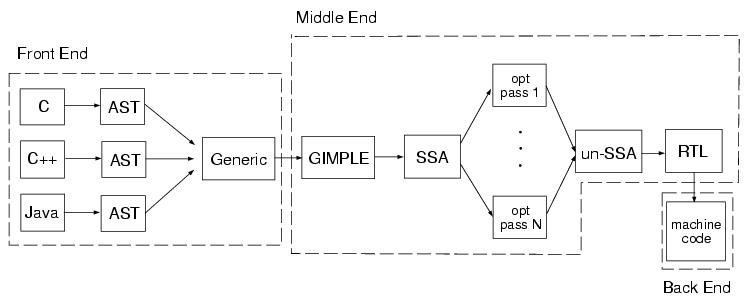
\includegraphics[height=50mm]{Figures/Gcc.jpg}}
    \vspace{0cm}\caption{{\bf Gcc} compiler.}
    \label{fig:Gcc}
\end{figure}

%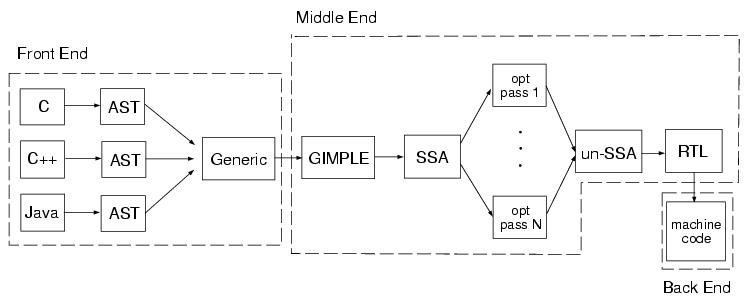
\includegraphics[height=60mm]{Figures/Gcc.jpg}

There is a book describing the compiler internals for versions 3.4 and
4.1~\cite{Stallman:2009}, although in 2018 distributions are for
versions 7, 8 and upcoming 9 (accessible in {\sc SVN})~\cite{Stallman:2018}.
The compressed ({.tar.gz}) source code is 80MB (8.2.0), 535MB.  The document for
the upcoming release 9 is essentially a listing of functions with a single line
description for each function.

%"GNU Compiler Collection Internals", Richard Stallman, Oct 2018, (9.0.0 pre-release).
%"From Source to Binary: The Inner Workings of GCC", Red Hat Magazine, number 2, Dec 2004.

The best, with thousands of generic and architecture specific optimizations,
but it is a monster!  Very big, lots of people change it and maintain
it, making the code very volatile, since the user must keep up to constant
changes in the code.  The purpose is not code optimization since {\it Versat} does
not provide alternative instructions for its operations, only {\it picoVersat}
could benefit of {\bf gcc} features.  It provides {\tt asm} support and many other
{\bf gcc} specific {\bf C} language extensions.

\subsection{llvm}

\begin{figure}[!htbp]
    \centerline{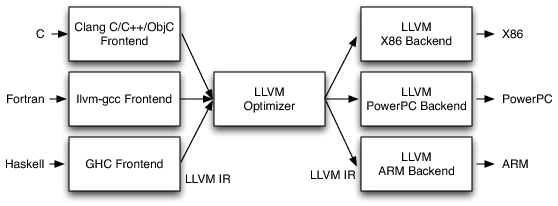
\includegraphics[height=45mm]{Figures/LLVMCompiler1.png}}
    \vspace{0cm}\caption{{\bf LLVM} compiler.}
    \label{fig:LLVM}
\end{figure}

%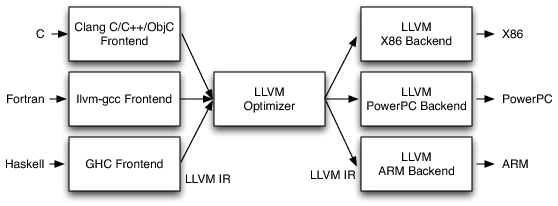
\includegraphics[height=50mm]{Figures/LLVMCompiler1.png}

{\sc LLVM} ({\em Low Level Virtual Machine}) was born as an infrastructure for
optimization from the masters thesis of Chris Lattner at the University of
Illinois at Urbana-Champaign~\cite{llvm:msc,Lattner04}.  Although an effort was
made to integrate it into {\bf gcc} it evolved into a full compiler with many
{\it front-ends}.  The first version was published Oct 24, 2003 with four releases
in 2018.  Many contributions for the compiler tool-chain were made over
the year, resulting in over 250 publications ({\tt http://llvm.org/pubs/}).

Nowadays, the code is extensive.  Only the core is 27MB compressed, resulting in
almost 7 million lines of code occupying 296 MB
(7.0.0)\footnote{http://releases.llvm.org/}.  The {\bf C} language
compiler ({\bf clang}) is roughly half the size.  Other {\it front-ends} include {\bf
  C++}, {\bf Objective C} and {\bf Fortran} among others.  It provides {\it back-ends}
for many processors: {\bf X86}, {\bf X86-64}, {\bf PowerPC}, {\bf PowerPC-64},
{\bf ARM}, {\bf Thumb}, {\bf SPARC}, {\bf Alpha}, {\bf CellSPU}, {\bf MIPS},
{\bf MSP430}, {\bf SystemZ}, and {\bf XCore}~(see Figure~\ref{fig:LLVM}).  A new
target description is provided by a declarative domain-specific language
processed by the {\bf tblgen} tool, similar to {\bf burg} grammar descriptions.
It features a stable internal instruction set implementation and documentation.

The compiler supports {\tt asm} directive extension and checks the correctness
of the embedded assembler itself.

It is still very large and difficult to manipulate.  The interface is complex,
written in {\bf C++}, but stable.  Requires a big effort for a single person for
a few months.

%"LLVM: A Compilation Framework for Lifelong Program Analysis \& Transformation"
%Chris Lattner and Vikram Adve
%Proc. of the 2004 International Symposium on Code Generation and Optimization (CGO'04), Palo Alto, California, Mar. 2004.
%
%"LLVM: An Infrastructure for Multi-Stage Optimization"
%Chris Lattner
%Masters Thesis, Computer Science Dept., University of Illinois at Urbana-Champaign, Dec. 2002.
%asm, -S, checks asm string!

\subsection{lcc}\label{lcc}

The {\bf lcc} is a {\bf C} compiler developed after the publication of the
{\bf BURG} papers by Proebstring, Hanson and Fraser in 1992, as a
demonstration of the concept~\cite{Fraser:burg,Fraser:gen92,Proebsting:2002}.
Up to that time {\it back-end}
compiler writing was an art.  The {\bf burg} concept allowed to describe the
target architectures in a single file as well as maintaining all of them in a
single executable, a retargetable compiler.  The target architecture is
selectable by a command line option.

Only the {\bf C} {\it front-end} is supported with a custom made lexical analyzer and
a {\bf yacc} parser~(see Figure~\ref{fig:lcc}).  The language is described in an
{\sc AST} with a well documented 32 instruction set.  Optimizations are
performed in the {\sc AST}, and through common sub-expression analysis, the tree
is converted into a {\bf DAG} ({\em Directed-Acyclic Graph}), although the
original tree is still accessible.

\begin{figure}[!htbp]
    \centerline{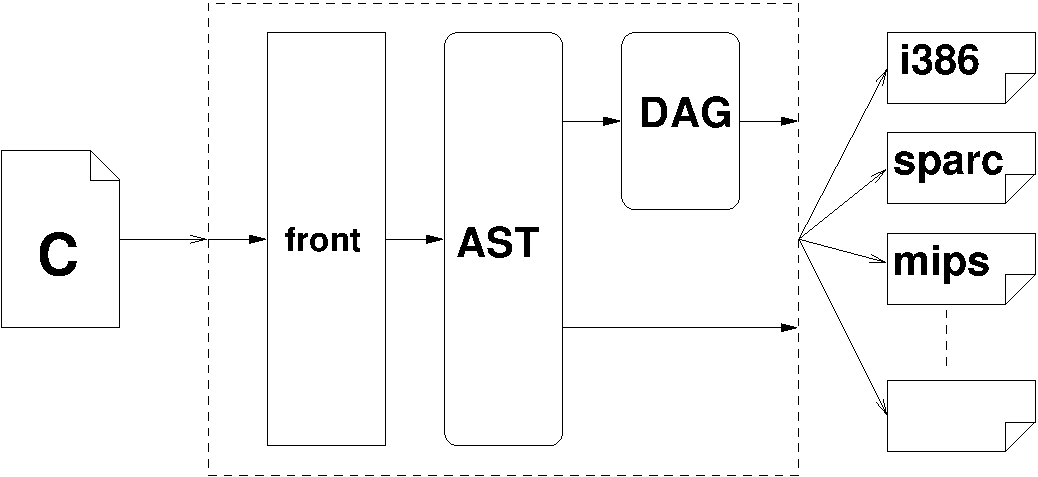
\includegraphics[height=45mm]{Figures/lcc.pdf}}
    \vspace{0cm}\caption{{\bf lcc} compiler.}
    \label{fig:lcc}
\end{figure}
%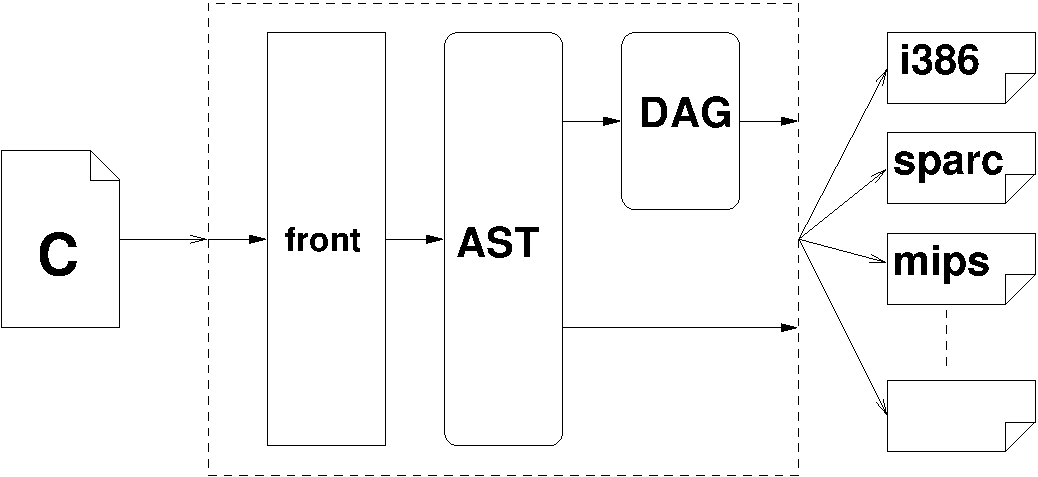
\includegraphics[height=50mm]{Figures/lcc.pdf}

A single {\bf C} {\it front-end} reduces the complexity and line count.  Simple to
introduce new {\it back-end} since it was designed to be retargetable.  A detailed and
extensive book and well defined {\it back-end} interface provide a good work
basis~\cite{hanson95}.  It provides no {\tt asm} directive and it's introduction
will require changes to core of the {\it front-end} code.  However, the compiler core
is composed of 260K lines of code and any changes should be
accessible~\footnote{https://github.com/drh/lcc}.
%626KB 260Kl 4MB
%no asm (doable)), with -S

\subsection{tcc}

The {\bf tcc} ({\em Tiny C Compiler}) is a small and fast {\bf C} compiler
written by Fabrice Bellard that began as the winner of a 2001 contest to
provide the smallest self-compiling language
({\sc OTCC})\footnote{https://bellard.org/otcc/}.
% https://bellard.org/tcc/tcc-doc.html
Now it is a full {\sc ANSI} {\bf C} compiler~\cite{Wheeler:2005} in 620KB of compressed code, totaling 105 thousand lines of code
(1.7MB)~\footnote{https://bellard.org/tcc/}.  It also claims to be 9 times faster than {\bf gcc}.  It only supports
the {\sc ANSI} {\bf C} {\it front-end} with {\it back-ends} for {\bf x86}, {\bf x64} and
{\bf arm} architectures.  The {\bf tcc} {\tt -run} option allows the code to be
compiled directly into memory, and executed without producing output files since
it includes an assembler and linker ({\em self-relying}).


On the other hand, the compiler provides few optimizations and only simple
register allocation, but the output is quite efficient for most non production
applications.  Documentation is limited but the code is manageable, however no
{\tt asm} support is provided.  Also, the compiler produces binary code
directly, not output assembler code, and it might not be easy to add assembler
support altogether.

%no asm, no -S

\subsection{Portable C Compiler}

The {\bf pcc} was developed in the 1970s by Stephen Johnson of the Bell
Labs~\cite{Johnson:1978}.
It was one of the first compilers that could target different architectures.
{\bf pcc} was the {\sc BSD Unix} {\bf C} compiler until it was replaced by
{\bf gcc}.  A 2007 rewriting ported it to {\sc C99} standard.
In the present form, {\bf pcc} was released in 2011 and supports {\bf x86}
and {\bf x64} architectures. % http://pcc.ludd.ltu.se/
It provides {\tt asm} support, but relies on rather old technology with no
instruction selection tool, such as {\bf burg}.
On the other hand it comprises only 160K lines of
code~\footnote{http://pcc.ludd.ltu.se/}.
%asm, -S
%1M, 160Kl 4MB

\subsection{Amsterdam Compiler Kit} % http://tack.sourceforge.net/ https://github.com/davidgiven/ack

The Amsterdam Compiler Kit ({\sc ACK})~\cite{Tanenbaum:1983}, developed in
early 1980s, was one of the first retargetable compilers with {\it front-ends}
for {\bf C}, {\bf Pascal}, {\bf Modula-2}, {\bf Occam}, and {\bf BASIC} as well
as {\it back-ends} for many processors and micro-processors.
The technology used is outdated but simple and no {\tt asm}
is provided~\footnote{http://tack.sourceforge.net/}.
%no asm, no -S
%4MB, 700Kl, 22MB

%Tanenbaum, Andrew S; van Staveren, H.; Keizer, E.G.; Stevenson, J.W. (1983). "A Practical Tool Kit For Making Portable Compilers". Communications of the ACM. 26 (9): 654–660. doi:10.1145/358172.358182.

\subsection{Small device C compiler} % http://sdcc.sourceforge.net/

The {\bf sdcc} is an {\sc ANSI} {\bf C} retargetable
compiler~\cite{sandeep:2000}, written by Sandeep Dutta.
It targets many microprocessors but no major processors, although it can
be retargeted for other microprocessors. The list of targets is the following.

Intel {\sc MCS51} based microprocessors (8031, 8032, 8051, 8052, etc.), Maxim
(formerly Dallas)\linebreak
{\sc DS80C390} variants, Freescale (formerly Motorola) {\sc
  HC08} based (hc08, s08), Zilog Z80 based {\sc MCUs} (z80, z180, gbz80, Rabbit
2000/3000, Rabbit 3000A, {\sc TLCS-90}), and {\sc STMicroelectronics} {\sc
  STM8}. Work on the Microchip {\sc PIC16} and {\sc PIC18} is under development.

It does not support {\tt asm} directives and the code, although large (7M lines
of code), is essentially dedicated to each specific
processor~\footnote{http://sdcc.sourceforge.net/}.
%Sep 27th, 2018: SDCC 3.8.0 released.
%no asm, with -S
%18MB compressed, 7 Mlines, 220MB

\section{{\sc CGRA} Compilers}

Unlike the previous general purpose {\bf C} language compilers, {\sc CGRA}
compilers directly address the problem of configuration and reconfiguration of a
{\sc CGRA} platform.
%ver compiladores que estao no mail (TRIPS, IMAGINE, REMARC, RICA, PADDI, Chimaera, Montium, GARP, PipeRench, EGRA, SmartCell, PADDI, Pleiades, DRRA, Redefine, Colt, Matrix, FPCA, CGRA Express, and HARTMP)
%"Coarse Grained Reconfigurable Architectures in the Past 25 Years: Overview and Classification"
%%%

% refs/2013HSPSdesutter.pdf : Coarse-GrainedReconfigurableArray Architectures
%In general, the performance obtained on a programmable processor for a certain application can be defined as the reciprocal of the application execution time.
Some {\sc CGRAs}, like {\sc ADRES}, Silicon Hive, and MorphoSys are fully
dynamically reconfigurable: exactly one full reconfiguration takes place for
every execution cycle~\cite{DeSutter2010}.  Other {\sc CGRAs} like the
KressArray are fully statically reconfigurable, meaning that the {\sc CGRA} is
configured before a loop is entered, and no reconfiguration takes place during
the loop at all~\cite{DeSutter2010}.  Still other architectures feature a hybrid
reconfigurability. The RaPiD architecture features partial dynamic
reconfigurability, in which part of the bits are statically reconfigurable and
another part is dynamically reconfigurable and controlled by a small
sequencer~\cite{DeSutter2010}.  Most compiler research has been done to generate
static schedules for {\sc CGRAs}~\cite{DeSutter2010}.  Not enough details are
available in the descriptions of the compiling techniques, and few techniques
have been tried on a wide range of {\sc CGRA} architectures~\cite{DeSutter2010}.
For that reason, it is very difficult to compare the efficiency, effectiveness
and user interface of the different techniques, this is, compilation time,
quality of the generated code, and how easy it is to use and to port code to the
language used, respectively~\cite{Tuhin08}.

There are frameworks that try to compile code in usual languages to {\sc CGRAs}.
Most of these frameworks have however some limitations that do not allow them to
adapt the code fully to {\sc CGRAs}' purposes.  For example, the {\sc IMPACT}
compiler framework is used in order to parse {\bf C} source code and get the
Intermediate Representation ({\sc IR})~\cite{Mei03}.  We can then change what
the {\it back-end} does to this {\sc IR}, to get the desired result.  However,
because of the {\sc IMPACT} {\it front-end}, most algorithms can only handle
inner loops of loop nests~\cite{Mei03}.  And since changing the {\it front-end}
as well as the {\it back-end} is the same as creating a new compiler, most of
these frameworks have problems when there is a need to really adapt the code not
made in the specific assembly language of the {\sc CGRA} supposed to run the
code.

% refs/04b_2.pdf : Exploiting Loop-Level Parallelism on Coarse-Gained Reconfigurable Architectures Using Modulo Scheduling
%Arquitectures often consist of tens to hundreds of FUs that are capable of executiong word, or even subword level operations instead of bit-level ones, which are usually found in FPGAs.

%Some use structure (GUI based) design tools to manually generate design (limits size of desing)[19, 5].
%Some use Instruction Level Paralelism (ILP) (limited scope and doesn't use architecture efficiently which means it can not reach a higher level of paralelism than a VLIW)[4, 12].
%Some use Loop-Level Paralelism (LLP), applying pipelining (suffers from applicability limitations)[3, 9, 18].

%Limitations:
%It's more time consuming compared to a typical scheduling algorithm of a compiler.
%Can not handle pipelined FUs and limited register files.
%Overall negative impact on the performance of the application.


% refs/99.pdf : Graph Minor Approach for Application Mapping on CGRAs

Nowadays most of the algorithms used for {\sc CGRAs} are adaptations of the ones
used for {\sc FPGAs} but, since the structure is not the same, this approach is
not the most efficient and/or effective~\cite{Chen14}.

%The most widely applicable static scheduling techniques use different forms of Modulo Resource Routing Graphs (MRRGs).

\subsection{Comparative Analysis}

Compilers are complex tools.  However, if the target processor is simple and the
high-level language is limited, a simple compiler can be developed in a few
months, using the right tools.  For large and complex languages like {\bf C},
with a large population of skilled programmers, a number of freely available
compilers exist.  The development of a compiler, even with powerful tools, is a
very complex and time consuming task, that usually involves tens of persons.
For large and complex languages like {\bf C} the use of an existing
infrastructure is of prime importance.

The {\bf B} programming language is a good choice if changes to the {\it front-end} of
the compiler are necessary, since changing the {\it front-end} as well as the {\it back-end}
is essentially writing a completely new compiler.

More complex languages, like {\bf C++}, are an overkill for a processor with
limited memory like {\it Versat} since with its memory limitations it will not
be able to run large object-oriented programs.

% why was lcc the choice... (in next section)

\cleardoublepage

%%%%%%%%%%%%%%%%%%%%%%%%%%%%%%%%%%%%%%%%%%%%%%%%%%%%%%%%%%%%%%%%%%%%%%%%
%                                                                      %
%     File: Thesis_Implementation.tex                                  %
%     Tex Master: Thesis.tex                                           %
%                                                                      %
%     Author: João D. Lopes                                            %
%     Last modified :  7 July 2017                                     %
%                                                                      %
%%%%%%%%%%%%%%%%%%%%%%%%%%%%%%%%%%%%%%%%%%%%%%%%%%%%%%%%%%%%%%%%%%%%%%%%

\chapter{Architecture}
\label{chapter:architecture}

Versat is designed for fixed-point signal processing and its
architecture is shown in figure~\ref{fig_top}. It can be used by host
processors in the same chip, as some procedures can run faster and at
lower energy on Versat.

In order to reduce the dependency on the host CPU, Versat features a
simple Controller used for algorithmic control, self-reconfiguration
and data movement. This frees the host for more useful tasks. The
controller is programmable and has an instruction memory where Versat
programs (aka kernels) are stored. Control over the different modules
is exerted using a Control Bus. Though not shown, there is also a
serial divider accessible from the Control Bus.

Versat has a special unit that performs data computation, the Data
Engine (DE). This unit is composed of Functional Units (FUs)
interconnected by a full mesh. Hence, there is more than one way to
make a given datapath, which is useful for simplifying the compiler.

The Configuration Module (CM) holds the configuration of the DE, i.e.,
it specifies the current datapath, and has another register where the
next configuration of the DE can be prepared; it can also temporarily
store tens of other complete configurations, which can be switched at
runtime. The Controller can write partial configurations to the CM,
and can also save and restore entire configurations from the
configuration memory.

\begin{figure}[!htb]
\centering 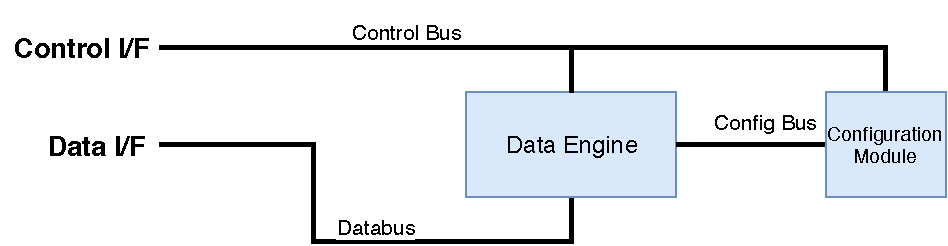
\includegraphics[width=0.70\textwidth]{drawings/top.pdf}
\caption{Versat top-level entity.}
\label{fig_top}
\end{figure}

Versat has a DMA module so it can independently and efficiently
transfer data, programs and configurations in and out of the
device. The DMA drives a master Advanced Extensible Interface --
AXI4. It is an interface designed by ARM, which derives from the
Advanced Microcontroller Bus Architecture (AMBA).

To communicate with the host processor, Versat has a shared Control
Register File (CRF). The CRF has two host interfaces that can be
selected at compile time: a Serial Peripheral Interface (SPI) and a
parallel bus interface. The SPI slave interface is used when the host
system is an off-chip master device. The SPI interface is mainly used
for debug and testing purposes. The parallel bus interface is used
when the host is some embedded processor and may be supplied in the
AXI4 Lite format.


%%%%%%%%%%%%%%%%%%%%%%%%%%%%%%%%%%%%%%%%%%%%%%%%%%%%%%%%%%%%%%%%%%%%%%%%
\section{Data Engine}
\label{section:dataEngine}

The Data Engine (DE) has a fixed topology comprising 15 Functional
Units (FUs) as shown in figure~\ref{fig_de}. The DE is a 32-bit
architecture and contains the following configurable FUs: 4 dual-port
embedded memories ($8kB$ each), 6 Arithmetic and Logic Units (ALUs), 4
multipliers and 1 barrel shifter. The output register of the FUs and
the embedded memories are accessible by the Controller for reading and
writing. (The embedded memory blocks are treated like any other FU by
the Versat tools.)

\begin{figure}[!htb]
\centering
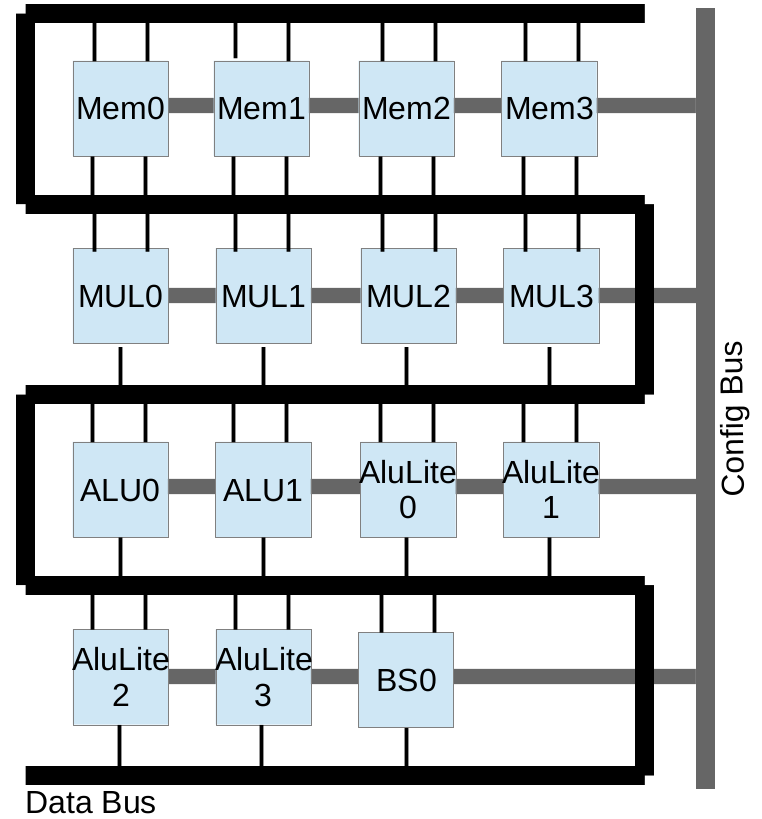
\includegraphics[width=0.75\textwidth]{drawings/de.pdf}
\caption{Data engine.}
\label{fig_de}
\end{figure}

\subsection{DE Structure}
\label{subsection:DEStructure}

In the DE, the FUs are interconnected by a wide bus called the Data
Bus. The Data Bus is simply the concatenation of all FU outputs. Each
FU output contributes a 32-bit section to the Data Bus, except the
embedded memories that contribute 2 sections with their 2
ports. According to the number of FUs of each type given before, the
Data Bus has $2\times4+6+4+1=19$ sections of 32 bits. In addition to
FU outputs, the Data Bus has 2 fixed sections containing the constants
0 and 1, which have been added because they are commonly used in
datapaths. Each FU input can select any of these sections and there is
also a selection that ignores the input value so that FU can be used
as a Controller shared register. The FUs take their configurations
from the respective configuration registers in the CM, whose outputs
are concatenated in another wide bus denoted the Config Bus. There is
a fixed set of high-level operations available in each FU. For
example, an ALU can be configured to perform addition, subtraction,
several logical functions, maximum, minimum, among others.

In figure~\ref{fig_fu}, it is shown in detail how a particular FU is
connected to the control, data and configuration buses. The FU, of
type ALU, is labeled FU5 and has 2 pipeline stages. The last pipeline
stage, denoted {\tt pipeline register 1}, stores the output of the
ALU, drives one section of the Data Bus and can be read or written by
the Controller using the Control Bus (as shown in the figure). This
feature enables the FUs to be used as Controller/DE shared
registers. Each FU5 input has a programmable multiplexer to select one
of the 19 sections of the Data Bus. Although the Config Bus is shown
going to all FUs, in fact only the configuration bits of each FU are
routed to it. These bits are called the {\em configuration space} of
the FU. The configuration space is further divided in several {\em
  configuration fields}, which are 3 in this example: the selection of
input A (5 bits), the selection of input B (5 bits) and the selection
of the function (4 bits). The partial reconfiguration scheme works at
the field level, so it is only possible to reconfigure these fields
individually.

\begin{figure}[!htb]
\centering
\includegraphics[width=0.85\textwidth]{drawings/FU.pdf}
\caption{Functional unit detail.}
\label{fig_fu}
\end{figure}

Since any FU can select any FU output as one of its inputs, then the
DE has a {\em full mesh topology}. This may seem exaggerated and
unnecessary but this topology accomplishes 2 major goals: (1) {\em an
  intuitive assembly programmer's model is achieved}; (2) {\em the
  compiler design is greatly simplified}. In fact, assembly
programmers need not remember or check what is connected to what since
everything is connected to everything. Hardware datapaths can be
manually built using store instructions that write to the
configuration fields of the used FUs. A compiler can be developed with
less effort as complex place and route algorithms, commonly used in
CGRAs, become unnecessary with a fully connected topology.

Assembly programmability is a powerful feature. It may be used to
optimize critical program sections or to work around bugs. In fact,
hardware bugs, defects or failures may eventually be circumvented at
post-silicon time using assembly code to avoid using the troubled
parts of the architecture. Compiler problems can also be fixed by
replacing the failing high-level code with assembly code.

In other approaches, such as in~\cite{Mei05}, a full mesh topology
would be problematic because of the cycle by cycle reconfiguration. It
causes frequent switching of the interconnect network and consequent
power dissipation. However, in Versat, reconfiguration does not happen
every clock cycle. The interconnect consumes very little power since
Versat is reconfigured only after a complete program loop or two
levels of nested loops are executed in the DE. It may also be argued
that a full mesh topology is large and limits the frequency of
operation. However, our IC implementation results indicate that only
$4.04\%$ of the core area is occupied by the full mesh interconnect,
while the core can work at a maximum frequency of $170MHz$ in a
$130nm$ process. This is sufficient for many target applications. For
example, in the multimedia space, some applications are required to
work at an even lower frequency because of power and energy
constraints.

Each configuration of the DE can implement one or more hardware
datapaths. Multiple datapaths operating in parallel realize
Thread-Level Parallelism (TLP). Datapaths having identical parallel
paths implement Data-Level Parallelism (DLP). Finally, datapaths
having long FU pipelines exploit Instruction-Level Parallelism (ILP).

In figure~\ref{fig_de_dp}, three example hardware datapaths are
illustrated. Datapath (a) implements a pipelined vector
addition. Despite the fact that a single ALU is used, ILP is being
exploited as the memory reads, addition operation and memory write are
being executed in parallel for consecutive elements of the
vector. Datapath (b) implements a vectorized version of datapath (a)
to illustrate DLP combined with the ILP. The vectors to be added
spread over memories M0 and M2, so that 2 additions can be performed
in parallel. ILP and DLP can be further exploited as in datapath (c),
whose function is to compute the inner product of two vectors: four
elements are multiplied in parallel and the results enter an adder
tree with an accumulator at the root. When an ALU is used as an
accumulator the unused data input is used as a control input. As seen
in the figure, this input is kept with the value 0, which specifies
the accumulator function. Any positive value specifies this function
while a negative value specifies that the ALU simply registers the
data input.

\begin{figure}[!htb]
\centering
\includegraphics[width=0.85\textwidth]{drawings/datapaths.pdf}
\caption{Data engine datapaths.}
\label{fig_de_dp}
\end{figure}


%%%%%%%%%%%%%%%%%%%%%%%%%%%%%%%%%%%%%%%%%%%%%%%%%%%%%%%%%%%%%%%%%%%%%%%%
\subsection{Address Generation Unit}
\label{subsection:addressGenerationUnit}

Versat has 4 dual-port Random Access Memories (RAMs) of size 2048
words by 32 bits, which work normally as vector registers. Each port
has an input, an output and an address input equipped with an Address
Generation Unit (AGU), as shown in figure~\ref{fig_dpram}. The AGUs
can be programmed to generate an address sequence for accessing data
from the memory port during the execution of a program loop. Our AGU
scheme is similar to the one described in~\cite{Farahini14}, in the
sense that both schemes use parallel and distributed AGUs. The AGUs
support two levels of nested loops, with the restriction that the
inner loop has a maximum of 32 iterations and the outer loop has a
maximum of 2048 iterations. To compute longer loops reconfiguration is
needed. AGUs can start execution with a programmable delay, so that
circuit paths with different accumulated latencies can be
synchronized. Each AGU can be operated independently from the other
AGUs, which allows TLP in the DE.

\begin{figure}[!htb]
\centering
\includegraphics[width=0.45\textwidth]{drawings/dpram.pdf}
\caption{Dual-port embedded memory with AGUs.}
\label{fig_dpram}
\end{figure}

Datapath (b) in figure~\ref{fig_de_dp}, previously used to explain
DLP, can also be used to explain TLP as follows. Suppose one block of
vector elements to be added is placed in memory M0, and that its
address generators M0-A, M0-B and M1-A are started (Thread 1). In
parallel, one can move the next block to memory M2 and start AGUs
M2-A, M2-B and M1-B (Thread 2). The user program can monitor the
completion of these threads and restart them with new vector
blocks. In this way, vectors that largely exceed the capacity of the
DE memories can be processed in a continuous fashion.

\begin{table}[!htb]
  \renewcommand{\arraystretch}{1.2} % more space between rows
  \caption{Address generation unit parameters.}
  \label{tab:MemParameter}
  \centering
  \begin{tabular}{lcp{10cm}}
    \toprule
    Parameter & Size (bits) & Description\\
    \midrule
    Start     &          11 & Memory start address. Default value is 0. \\
    Per       &           5 & Number of iterations of the inner loop, aka Period. Default is 1 (no inner loop). \\
    Duty      &           5 & Number of cycles in a period (Per) that the memory is enabled. Default is 1.\\
    Incr      &          11 & Increment for the inner loop. Default is 0.\\
    Iter      &          11 & Number of iterations of the outer loop. Default is 1.\\
    Shift     &          11 & Additional increment in the end of each period. Note that Per+Shift is the increment of the outer loop. Default is 0.\\
    Delay     &           5 & Number of clock cycles that the AGU must wait before starting to work. Used to compensate different latencies in the converging branches of the configured hardware datapaths. Default is 0.\\
    Reverse   &           1 & Bit-wise reversion of the generated address. Certain applications like the FFT work with mirrored addresses. Default is 0.\\
    \bottomrule
  \end{tabular}
\end{table}

The AGU parameters control the generation of address sequences and are
described in~Table~\ref{tab:MemParameter}. With these parameters the
AGU can generate an address sequence for an embedded memory port. An
example address sequence is shown in figure~\ref{fig_addrgen}. Note
that the AGU is enabled with a Delay of 2 clock cycles. It is enabled
periodically for $Duty=3$ cycles after every $Per=5$ cycles. The
initial value of the sequence is given by $Start=10$ (in decimal
notation). Every enabled cycle it is incremented by $Incr=2$; in the
last cycle of a period it is incremented by $Incr+Shift=-3$. This
pattern repeats for $Iter$ iterations, though this parameter is not
illustrated in the figure.

\begin{figure}[!htb]
\centering
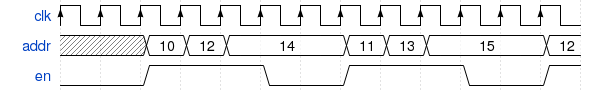
\includegraphics[width=0.75\textwidth]{drawings/addrgen.png}
\caption{AGU output for $Delay=2$, $Per=5$, $Duty=3$, $Start=10$, $Incr=2$, and $Shift=-5$.}
\label{fig_addrgen}
\end{figure}

The embedded memory ports have their own configuration fields: one for
selecting/disabling the input or outputting the generated sequence
(sel) and another for bypassing the AGU (Ext). If the input is
disabled then the port is enabled for reading. If it is selecting a
data source, then it is enabled for writing but also reads the word
previously stored at that address. Normally an AGU is used for
generating an address sequence for the memory port. However, the port
can also be configured to output the generated sequence to the DE,
where it can be used for general purposes. With this feature, data
patterns, synchronization and control signals can be generated for the
FUs. The configuration for bypassing the AGU ($Ext=1$) enables the
port to use as address values computed by datapath. In this case the
port address is input by the other port of the same memory. This
feature provides Versat with the capability of working with pointers.

In summary, the two memory ports can be independently configured to
read and/or write the memory, each memory port can be read/written with
an address sequence computed by the AGU or by some datapath in the
DE, and a memory configured for writing also reads the previously
stored word from the same address with one clock cycle of latency.

%%%%%%%%%%%%%%%%%%%%%%%%%%%%%%%%%%%%%%%%%%%%%%%%%%%%%%%%%%%%%%%%%%%%%%%%
\subsection{Arithmetic and Logic Unit}
\label{subsection:arithmeticLogicUnit}

There are two types of Arithmetic and Logic Units (ALUs), denoted Type
I and Type II: 2 Type I and 4 Type II. Both types have two inputs, A
and B, and an output Y.  A summary of the ALU operations is given in
Table~\ref{tab:AluOpers}. The ALUs have 4 configuration bits for the
operation field and thus can support 16 different operations.

\begin{table}[!htb]
  \renewcommand{\arraystretch}{1.2} % more space between rows
  \caption{ALU functions.}
  \label{tab:AluOpers}
  \centering
  \begin{tabular}{lll}
    \toprule
    Operation              &                Type I & Type II (w/ feedback)\\
    \midrule
    Logic OR               &           Y = A $|$ B & Y = Y $|$ B\\
    Logic AND              &            Y = A \& B & Y = Y \& B\\
    Logic XOR              &      Y = A $\oplus$ B & NA\\
    Addition               &             Y = A + B & Y = (A$<$0)? B: Y+B\\
    Subtraction            &             Y = B - A & Y = (A$<$0)? B: Y-B\\
    Multiplexer            &     Y = (A$<$0)? B: 0 & Y = (A$<$0)? B: Y\\
    Sign extend 8          &    Y = A[7]...A[7..0] & NA\\
    Sign extend 16         &  Y = A[15]...A[15..0] & NA\\
    Shift right arithmetic & Y = {A[31], A[31..1]} & NA\\
    Shift right logical    &   Y = {'0', A[31..1]} & NA\\
    Signed compare         &       Y[31] = (A$>$B) & Y[31] = (Y$>$B)\\
    Unsigned compare       &       Y[31] = (A$>$B) & NA\\
    Count lead zeros       &            Y = CLZ(A) & NA\\
    Signed maximum         &            Y=max(A,B) & Y = (A$<$0)? Y: max(Y,B)\\
    Signed minimum         &            Y=min(A,B) & Y = (A$<$0)? Y: min(Y,B)\\
    Absolute value         &             Y=$|$A$|$ & NA\\
    \bottomrule
  \end{tabular}
\end{table}

Type II ALUs use one of the configuration bits to create an internal
feedback loop from the output to input A. With the other 3 bits, Type
II ALUs can support 8 operations. If the feedback bit is set to '0',
these operations are the same as for Type I ALUs. If the feedback bit
is set to '1', the operation has input B and the current output as
operands. In this case, input A becomes available for runtime control
of the ALU, which is used for implementing conditional statements in
operations ADD, SUB, MUX, MIN and MAX. For instance, the addition
operation (ADD) can be turned into a conditional accumulate operation:
the ALU accumulates the values coming to input B, if input A is not
negative or simply registers input B otherwise. In another example,
the signed minimum operation can be used to detect and register the
minimum value among only certain elements of a sequence coming to
input B, by using input A as a data qualifier. Often, an AGU is used
to generate control sequences for the control input A of an ALU. The
type II ALU is an original way to enable conditional execution in the
DE.

%%%%%%%%%%%%%%%%%%%%%%%%%%%%%%%%%%%%%%%%%%%%%%%%%%%%%%%%%%%%%%%%%%%%%%%%
\subsection{Multiplier and Barrel Shifter}
\label{subsection:multiplierBarrelShifter}

The multiplier produces a 64-bit result from two 32-bit operands and
has two configuration parameters. One parameter allows selecting the
lower or higher 32 bits of the result. The other parameter forces the
multiply result to be left shifted by 1 bit. This configuration is
useful when operands are in the Q1.31 fixed-point format, which is
used in many DSP algorithms. By setting the first parameter to select
the high part of the result and the second parameter to left shift it
by 1, the multiplication of two Q1.31 operands also yields a Q1.31
result.

The barrel shifter can perform left and right shifts. Right shifts can
be configured as logical (no sign extension, feed '0' to the left) or
arithmetic (with sign extension). One configuration parameter
determines the shift direction (left or right) and another parameter
sets the right shift type (arithmetic or logic). In one input of the
barrel shifter is the value to be shifted and in the other input is
the shift size (0 to 31).

%%%%%%%%%%%%%%%%%%%%%%%%%%%%%%%%%%%%%%%%%%%%%%%%%%%%%%%%%%%%%%%%%%%%%%%%
\subsection{Functional Unit Latencies}
\label{subsection:functionalUnitLatencies}

Each FU has a latency due to pipelining: 2 clock cycles for the ALUs,
3 for the multipliers and 1 for the barrel shifter and embedded
memories. When configuring a datapath in the DE, it is necessary to
take into account the latency of each branch, and compensate for any
mismatches when branches with different latencies converge. To do
this, the AGUs have the {\em Delay} parameter explained in
Table~\ref{tab:MemParameter}. The branch latency is the sum of its FU
latencies.

%%%%%%%%%%%%%%%%%%%%%%%%%%%%%%%%%%%%%%%%%%%%%%%%%%%%%%%%%%%%%%%%%%%%%%%%
\subsection{Data Engine Control}
\label{subsection:dataEngineControl}

The DE is controlled using its Control and Status registers. The
Control register structure is the following: bit 0 (init) resets the
selected memory ports and bit 1 (run) enables the selected ports,
resets the selected FUs and starts the DE; bits~2~-~20 select the
memory ports and FUs to reset or enable. Recall there are 8 memory
ports and 11 other FUs in a total of 19 FUs to control. The Status
register structure is the following: bits~0~-~7 indicate which AGUs
are running (logic '0') or idle (logic '1').

%%%%%%%%%%%%%%%%%%%%%%%%%%%%%%%%%%%%%%%%%%%%%%%%%%%%%%%%%%%%%%%%%%%%%%%%
\section{Configuration Module}
\label{section:configuration}

The Configuration Module (CM) is composed of a Configuration Register
File used to prepare the next configuration, the Configuration Shadow
Register which holds the configuration being executed by the DE, and
the Configuration Memory where frequently used configurations are
stored (figure~\ref{fig_conf}). Configurations stored in the
configuration memory can later be used without modifications or they
can be partially reconfigured before used.

The configuration register file is divided in configuration spaces
which in turn are divided in configuration fields. Different
configuration spaces differ on the number of fields and configuration
fields differ on the number of bits. A full DE configuration is 672
bits. The configuration register file is addressable at the
configuration field level and there are 118 configuration fields. This
feature takes advantage of the fact that in most applications there is
a high likelihood that a certain configuration or a similar one will
be reused (time locality) to make partial reconfiguration effective.

The configuration shadow register holds an active configuration word
for the DE, which is copied from the configuration register file
whenever the Update signal is asserted by the Controller. Thus, the
contents of the configuration register file can be changed while the
configuration shadow register keeps the DE configured and running.

\begin{figure}[!htb]
\centering 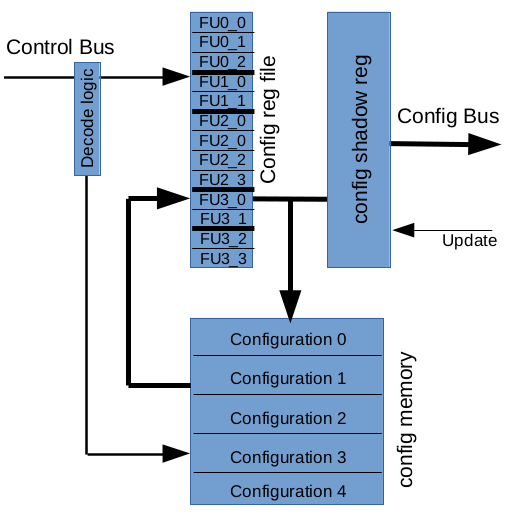
\includegraphics[width=0.8\textwidth]{drawings/conf.pdf}
\caption{Configuration Module.}
\label{fig_conf}
\end{figure}

The configuration memory is a dual-port 64-position memory, where each
position can store a full configuration and is, hence, 672 bits
wide. Configurations can be loaded/stored from/to the configuration
register file in just 1 clock cycle using one the memory ports. The
other port is 32-bit wide and used to load and store configurations in
the external memory using the DMA. This way, the configuration memory
can be extended beyond the 64 configurations. This scheme is designed
so that one can study the difference between working with pre-built
configurations stored in external memory and generating configurations
using the Versat controller.

%%%%%%%%%%%%%%%%%%%%%%%%%%%%%%%%%%%%%%%%%%%%%%%%%%%%%%%%%%%%%%%%%%%%%%%%
\section{Controller}
\label{section:controller}

The Versat Controller has a minimal architecture
(figure~\ref{fig_control}) to support reconfiguration, data movement,
algorithm control and host interaction. It contains 3 main registers:
the Program Counter (PC), the Accumulator Register (RA) and the
Address Register (RB). The PC contains the address of the next
instruction as usual. Register RA is the destination of all operations
that the controller performs, and is also often one of the operands
(accumulator architecture). Register RB is addressable by the
Controller and is used to store addresses for implementing indirect
loads and stores.

\begin{figure}[!htb]
\centering 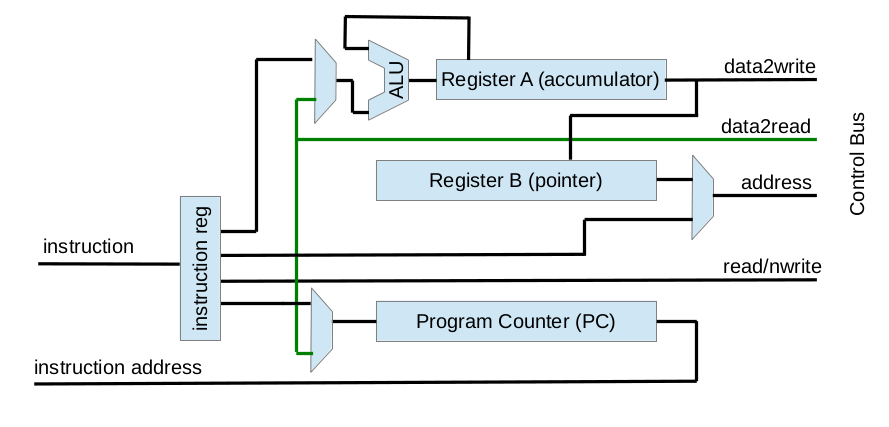
\includegraphics[width=0.95\textwidth]{drawings/control.pdf}
\caption{Controller.}
\label{fig_control}
\end{figure}

The controller has an instruction set of only 16 instructions ({\tt
  opcode} of 4 bits and {\tt Imm}ediate value of 16 bits). These allow
the controller to perform the following actions: loads/stores to/from
the accumulator, arithmetic/logic operations and branches. There are
three types of load instructions: of immediate constants, direct (from
an immediate address) and indirect from an address stored in register
RB. Store instructions can be direct or indirect.

The instruction set is outlined in Table~\ref{tab:isa}. As usual,
square brackets represent memory positions. For example, M[Imm]
represents the contents of the memory position whose address is
Imm. The PC is incremented for every instruction, except when
indicated otherwise (branch instructions).

\begin{table}[!htb]
  \renewcommand{\arraystretch}{1.2} % more space between rows
  \caption{Instruction set.}
  \label{tab:isa}
  \centering
  \begin{tabular}{cl}
    \toprule
    Instruction & Description\\
    \midrule
    nop   & No-operation\\
    rdw   & RA = M[Imm]\\
    wrw   & M[Imm] = RA\\
    rdwb  & RA = M[RB]\\
    wrwb  & M[RB] = RA\\
    beqi  & RA == 0? PC = Imm: PC += 1; RA = RA-1\\
    beq   & RA == 0? PC = M[Imm]: PC += 1; RA = RA-1\\
    bneqi & RA != 0? PC = Imm: PC += 1; RA = RA-1\\
    bneq  & RA != 0? PC = M[Imm]: PC += 1; RA = RA-1\\
    ldi   & RA = Imm\\
    ldih  & RA[31:16] = Imm\\
    shft  & RA = (Imm $<$ 0)? RA $<<$ 1: RA $>>$ 1\\
    add   & RA = RA + M[Imm]\\
    addi  & RA = RA + Imm\\
    sub   & RA = RA - M[Imm]\\
    and   & RA = RA \& M[Imm]\\
    \bottomrule
  \end{tabular}
\end{table}

In order to reduce the critical path and increase the clock frequency,
a pipeline register has been added between the instruction memory and
the instruction decoder. The controller then takes 2 clock cycles to
fetch an instruction, one from the memory itself and the other from
the instruction register shown in figure~\ref{fig_control}. For
simplicity, it executes every instruction fetched and thus branch
instructions have 2 delay slots. The delay slots can be filled with
useful instructions or with no operation (NOP) instructions.  For
instance, in a {\tt for} loop, the delay slots can be used to
increment the iteration count.

The boot loader software handles host procedure calls. The host writes
the procedure parameters to the CRF and writes the program address to
R0 which triggers a jump to the program address. During the execution
of a typical program, the DMA and the DE are used multiple times. DMA
and DE threads are spawned, hiding part of the controller execution
time, as shown later. This architecture allows programs to execute
precise time delays using a {\tt for} loop with a variable number of
instructions in its body. These instructions may be useful ones
(reconfiguration instructions, for instance) or just NOP instructions.

%%%%%%%%%%%%%%%%%%%%%%%%%%%%%%%%%%%%%%%%%%%%%%%%%%%%%%%%%%%%%%%%%%%%%%%%
\section{Divider}
\label{section:divider}

To perform divisions, Versat has a fixed-point serial divider, added
as a controller peripheral, which takes 33 cycles to complete one
division. It has shadow registers for the operands (dividend and
divisor), as well as for the results (quotient and remainder). This
means that it is possible to read the results and write next operands
while a new division is already being computed. It has one
configuration parameter that allows choosing between signed or
unsigned division. This implementation was designed for low energy and
small silicon area.

%%%%%%%%%%%%%%%%%%%%%%%%%%%%%%%%%%%%%%%%%%%%%%%%%%%%%%%%%%%%%%%%%%%%%%%%
\section{DMA}
\label{section:dma}

One of the crucial factors to guarantee acceleration is the rapidity
at which data is moved in and out of Versat. Accessing data words from
the external memory using load instructions is out of the
question. Data must be moved in large blocks using a DMA engine to
amortize the latency of the external memory device. The DMA engine is
operated by the Versat controller and transfers a data burst from
external memory into one of the Versat's memories (instruction,
configuration, or data engine memory) or vice versa.

From a Versat program point of view, the DMA is memory mapped and the
following DMA registers can be accessed: the external address
register, the internal address register, the size register, the
direction register, the status register and the start register. All
registers, except the status register, are duplicated allowing the
configuration of a new transaction while a previous one is
running. The external address register holds the transfer start
address in the external memory (32 bits), and the internal address
register holds the transfer start address in Versat (14 bits written
to a 32-bit register). The size register (8 bits) specifies the number
of words to be transferred (256 words maximum, as per the AXI4
interface). The direction register indicates if the transfer is from
Versat to external memory or vice-versa. After these registers have
been configured, the program writes anything to the start register and
the transfer begins. The contents of the status register tells the
program whether the DMA is still busy, done or if an error has
occurred.


%%%%%%%%%%%%%%%%%%%%%%%%%%%%%%%%%%%%%%%%%%%%%%%%%%%%%%%%%%%%%%%%%%%%%%%%
\section{Program memory}
\label{section:programMemory}

The Program Memory is divided in two parts: the boot ROM (256x32,
$1kB$) and the instruction memory RAM (2048x32, $8kB$). They are
addressable as a single memory: the first 256 addresses are used to
address the boot ROM, while the others are used to address the
instruction memory.

The boot ROM holds the code that allows Versat to communicate with the
host processor. Basically, it is used for the host to call Versat
kernels and to load/store values in any addressable memory position
within Versat without using the DMA. This includes loading programs
issuing store instructions to the Program Memory. However, the Program
Memory can not be read with load instructions. Its contents can only
be executed.


%%%%%%%%%%%%%%%%%%%%%%%%%%%%%%%%%%%%%%%%%%%%%%%%%%%%%%%%%%%%%%%%%%%%%%%%
\section{Control Register File}
\label{section:controlRegisterFile}

The 16x32 Control Register File (CRF) is implemented with a dual-port
register file (one port for the host and another for Versat). These
registers are shared between the host processor and Versat, which are
allowed to asynchronously read or write them.

\section{Qualitative comparison with other architectures}
\label{section:archComparisonWOtherArchitectures}

Versat has some distinctive features which can not be found in other
architectures: (1) it has a small number of FUs organized in a full
mesh structure; (2) it has a fully addressable configuration register
combined with a configuration memory to support partial configuration;
(3) it has a dedicated controller for reconfiguration, DMA management
and simple algorithm control -- no general purpose RISC~\cite{Lee00}
or VLIW~\cite{Mei05} processors are used.

CGRAs started as 1-D structures~\cite{Ebeling96} but more recently 2-D
square mesh FU arrays became more common~\cite{Lee00,Mei05,Liu15}. The
problem with square mesh topologies is that many FUs end up being used
as routing resources, reducing the number of FUs available for
computation and requiring sophisticated mapping
algorithms~\cite{Liu13}. Versat is an experiment on trading a lower FU
count with a richer interconnect structure. As explained before, the
silicon area occupied by the full mesh interconnect is less than $5\%$
and the limits placed on the frequency of operation are normally
irrelevant given the low energy budgets of target applications. In
fact, a low energy consumption often imposes a frequency of operation
which is well below Versat's maximum operating frequency.

As explained in~\cite{Liu15}, the reconfiguration time in CGRAs can
easily dominate the total execution time. To counter this effect
Versat takes partial reconfiguration to the extreme of using a fully
addressable configuration register. This keeps the reconfiguration
time to a minimum and contrasts with the more moderate hierarchical
reconfiguration scheme proposed in~\cite{Liu15}.

Since it is crucial to have reconfiguration done quickly, Versat
includes a small 16-instruction controller with low IO latency,
practically dedicated to reconfiguration management. This controller
is also used to manage data transfers and control the execution of
acceleration kernels. In other architectures~\cite{Lee00,Mei05,Liu15},
more comprehensive processors are used, which can also run complex
algorithms. However, combing complex application coding and
accelerator control is difficult. Using its controller, Versat can
completely take care of simple yet compute intensive kernels. Example
kernels are FFT, DCT, Motion Estimation, and even Big Data algorithms
such as K-Means Clustering. These kernels can simply be invoked by
host processors, and they will run in parallel to completion, without
requiring any external control.


\begin{comment}
After hardware reset the Versat, through boot ROM program, waits a
host command. Three registers of the CRF are used for this purpose:
one as a command register (R14), two as an address register (R0) and
another one as a data register (R15).

There are 3 commands (for now): read command, that allow the host to
access some data from Versat (for debug, for instance), write command,
that host uses to write some data into Versat, and run command, that
indicates to Versat to run some kernel.

In case of read, the host writes the read command into R14 (\#4), the
base address into R0 and waits that Versat write Acknowledge (Ack -
\#3) into R14. When it does, he read data from R15, clean Ack value
from R14 and waits for a new Ack. On Versat side, which is reading R0
until it has a nonzero value, after host command (written on R0), he
process the command given and get into a certain loop according the
command. In this case, after he loads the R0 value into RB, get into a
loop that reads R14 until it has a value that is not Ack. When this
happens, he checks if R14 value is equal to finish (\#2). If it is, go
back to boot ROM base address (cleans the R0 and wait it has a nonzero
value again), if not, read from the address pointed by RB, put the
data into R15, increment RB, write the Ack into R14 and go back to
read R14 loop (waits that R14 has a different value again).

In case of write, the host writes the first data value into R15, the
command into R14 and the base address into R0 (there is no write
command, it just have to be a different value that other commands uses
on protocol - i.e. \#0). When it does, he get into a loop that reads
R14 and wait for Ack. On Versat side, after processing the command
given, loads the R0 value into RB and get into a loop that reads R14
until it has a value that is not Ack. When this happens, he checks if
R14 value is equal to finish (\#2). If it is, go back to boot ROM base
address (cleans the R0 and wait it has a nonzero again), if not, write
R15 value into the address pointed by RB, increment RB, write the Ack
into R14 and go back to read R14 loop (waits that R14 has a different
value again).

For the execution of a kernel, the CRF is used by the host also to
pass parameters to Versat and by Versat to return status information
to the host (the registers used to do that are undefined, depends on
the kernel it self). After a host command, Versat do an unconditional
branch to address written on R0, starting the kernel execution.
\end{comment}

\cleardoublepage

%%%%%%%%%%%%%%%%%%%%%%%%%%%%%%%%%%%%%%%%%%%%%%%%%%%%%%%%%%%%%%%%%%%%%%%
%                                                                     %
%     File: Thesis_Development.tex                                    %
%     Tex Master: Thesis.tex                                          %
%                                                                     %
%     Author: Gonçalo Santos                                          %
%     Last modified : 28 May 2019                                     %
%                                                                     %
%%%%%%%%%%%%%%%%%%%%%%%%%%%%%%%%%%%%%%%%%%%%%%%%%%%%%%%%%%%%%%%%%%%%%%%

\chapter{Development}
\label{chapter:develop}

The {\bf lcc} compiler (see section~\cite{Fraser:1991b,lcc4}) is a
retargetable compiler with a single {\it front-end} for the {\bf C}
programming language ({\sc ANSI-C}).
As a retargetable compiler, multiple {\it back-ends} are available
and new ones can be easily added.
Currently, {\bf lcc} produces {\bf mips}, {\bf sparc} and
{\bf intel-x86} assembly, amongst other output formats.
Most formats, including the three referred, use an instruction
selector (see section~\ref{burg}) to generate and optimize the
output assembly code.
The {\bf lcc} compiler uses a specific instruction selection
tool ({\bf lburg}), included in the compiler distribution.
Ideally, the creation of a new {\it back-end} corresponds to an
{\bf lburg} grammar description, some auxiliary functions,
and a controlling structure.
A reference to the controlling structure is then inserted
into the {\tt src/bind.c} file and the {\bf makefile} update.

The {\bf lburg} grammar description file is composed of three
areas separated by a single line containing only the sequence
{\tt \%\%}, like other grammar description files for lexical
analysis (see section~\ref{lex}) or syntactic analysis
(see section~\ref{yacc}).
The first area contains declarations, the second area
contains the grammar, and the last area may contain
{\bf C} language functions and variables.
The declarations area includes a {\tt \%start} declaration,
{\tt \%term} declarations, and {\bf C} language declarations.
The {\tt \%start} declaration identifies the grammar
non-terminal that each {\sc AST} tree must produce,
based on the grammar tree patterns. If the start
non-terminal can not be produced from any combination
of the grammar rules, then an error is generated and
no output is produced. The {\it Versat} grammar uses
{\tt stmt}, or statement, as the start symbol for the grammar.
The {\tt \%term} declaration associates a symbolic name used
in the patterns of each rule with the number stored in the
terminal nodes of the tree ({\sc AST}) which represents
the program.
For instance, a tree node containing an integer of metric $1$,
usually a {\bf C} language {\tt char} type, is labeled with
the $1045$ value by the {\bf lcc} compiler, and associated
with the name {\tt CNSTI1} by the {\it Versat} {\it back-end}
with the declaration {\tt \%term CNSTI1=1045}.

The values that correspond to each terminal type in the
tree can be computed based on the operation, the data
type and the metric.
The operation is one of $35$ types of instructions
generated by the compiler for all {\bf C} language constructs.
The instruction are numbered from $1$ ({\tt CNST}) to $37$
({\tt LABEL}) and $44$ ({\tt VREG}).
The full list (see~\cite[p.84]{hanson95} include
{\tt CNST} (a literal constant),
{\tt ARG} (a function argument),
{\tt ASGN} (an assignment),
{\tt INDIR} (a pointer dereferencing),
{\tt CVF} (a conversion from floating point),
{\tt CVI} (a conversion from an integer),
{\tt CVU} (a conversion from an unsigned integer),
{\tt CVP} (a conversion from a pointer),
{\tt NEG} (the symmetric value),
{\tt CALL} (a function call),
{\tt LOAD} (a register movement),
{\tt RET} (the return from a function),
{\tt ADDRG} (address of a global variable),
{\tt ADDRF} (address of a function argument),
{\tt ADDRL} (address of a local variable),
{\tt ADD} (arithmetic sum),
{\tt SUB} (arithmetic subtraction),
{\tt LSH} (a left shift),
{\tt MOD} (division integer remainder),
{\tt RSH} (a right shift),
{\tt BAND} (a bit-wise and),
{\tt BCOM} (a bit-wise complement),
{\tt BOR} (a bit-wise inclusive or),
{\tt BXOR} (a bit-wise exclusive-or),
{\tt DIV} (arithmetic division),
{\tt MUL} (arithmetic multiplication),
{\tt EQ} (an equal comparison),
{\tt GE} (a greater or equal comparison),
{\tt GT} (a greater than comparison),
{\tt LE} (a less or equal comparison),
{\tt LT} (a less than comparison),
{\tt NE} (a not equal comparison),
{\tt JUMP} (an unconditional jump),
{\tt LABEL} (a global label),
{\tt VREG} (a register variable).
The data type can be {\tt F} (floating point),
{\tt I} (signed integer), {\tt U} (unsigned integer),
{\tt P} (any pointer type), {\tt V} (void) and
{\tt B} (structure type).
The metric is the size of the variable,
where {\tt sizeof(char)} must be $1$
(see~\cite[p.79]{hanson95})
as is required by the {\bf C} programming language.
However, not all instructions can be applied for all
data types, and are only available for some metric values.
For instance, {\tt ADDRG} only supports {\tt P} for
the processor word size, {\em i.e.} {\tt ADDRP4} for
a 32-bit machine and {\tt ADDRP8} for a 64-bit machine.
On the other hand, addition is supported for almost
all data types, except void and structure,
and all metrics.

The {\it Versat} {\it back-end} defines only metric
$1$ terminals since a character has metric $1$,
although it occupies 32-bits, as all other
integer data types.

\section{{\bf lcc} compiler interface}
% [asdl.pdf:6-7]
As referred, the {\it back-end} is registered in the
compiler by a single data structure,
{\tt Interface versatIR} in this case.
This structure defines the processor metrics.
In {\it Versat} all data types have a size
metric of $1$ except the {\bf long long},
{\bf double} and {\bf long double} that
should occupy $2$ words, although they
are currently not implemented.
All data types are word aligned, so the align
metric is always $1$.
These metrics correctly map address computations
but fail to address literals, since {\bf lcc}
assumes that a type {\tt char} is 8-bits and
its size is $1$ ({\tt sizeof(char)==1}).
Although this is true for most common computers
of today, old computers and specific processors
had different size words.
Processors, like {\it Versat}, that are not
used for general computing, do not have
different size data types.
Instead, all data types are 32-bits long,
which is a wast of space for character processing.

In order to circumvent the {\bf lcc} assumption
that characters are always 8-bits long, the
data types minimum and maximum values were
hacked for the {\it Versat} {\it back-end} in
the file {\tt types.c}:
\begin{Verbatim}[baselinestretch=1.2]
    types.c:42
        int i; for (i = 0; bindings[i].ir != IR; i++);
        int versat = !strcmp(bindings[i].name, "versat");
    types.c:51
        if (versat) p->u.limits.max.i = ones(32)>>1;
    types.c:56
        if (versat) p->u.limits.max.u = ones(32);
\end{Verbatim}

However, pointer literals are not computed from
data types but from metric sizes, assuming
8-bits per byte.
Since the code ({\tt 8}$^{\wedge}${\tt ty->size})
is spread out all over the compiler, a major
rewriting was needed.
Instead, pointer literals should be assigned to
integers and then converted into pointers, as
referred in the section~\ref{limitations}.
This is not a common {\bf C} operation, specially
in virtual memory machines, but is very useful in
the real memory mapped {\it Versat} architecture.
% metrics: 1 vs 4 in v[i] (delta=3072)

The {\it back-end} data structure also defines some
architecture requirements.
These include the endian number format representation
({\tt little\_endian=1} in {\it Versat}),
whether multiplication and division are executed
in hardware or by software libraries
({\tt mulops\_calls=1} or library in {\it Versat}),
whether the {\it back-end} can handle a {\bf DAG}
(directed acyclic graph), or only a tree
({\tt wants\_dag=0} or tree in {\it Versat}), or if
it can handle passing structures to and from
functions: {\tt wants\_callb=0} and {\tt wants\_argb=0}.
When the {\it back-end} does not handle structure
passing directly, the compiler
does not generate {\tt CALLB} or {\tt ARGB}
nodes, and block copies
must be handled by a {\tt blkloop} function.

The final part of the {\it back-end} data structure
defines a set of procedures to handle
specific parts of the code generation.
These include {\tt progbeg} (setup {\it back-end}),
{\tt progend} (finalize {\it back-end}),
{\tt rmap} (define a new register set),
{\tt segment} (change segment),
{\tt target} (assign register for specific instructions),
{\tt clobber} (spill registers before specific operations),
{\tt emit2} (emit code that can not handled by string template),
{\tt blkfetch} (block based fetch code),
{\tt blkstore} (block based store code),
{\tt blkloop} (memory block copy),
{\tt doarg} (register assignment to arguments),
{\tt local} (register assignment to locals),
{\tt function} (generate a function activation record),
{\tt defsymbol} (define a symbol),
{\tt  address} (compute an address),
{\tt defconst} (define a literal constant),
{\tt defaddress} (define an address),
{\tt defstring} (define an string),
{\tt export} (declare an exported symbol),
{\tt import} (declare an external symbol),
{\tt global} (declare a global symbol),
{\tt space} (reserve uninitialized data)
\cite[p.79]{hanson95}.

\section{Register assignment}

In order to implement the {\bf C} language constructs,
the processor must provide an accumulator to handle
return values from functions, a stack pointer to save
arguments, locals and spills, and a frame pointer to
access arguments and locals by a fixed amount.
All of these registers can be set in fixed memory positions,
but the execution degradation is significant.

% R0 cannot be used (picoversat/rtl/testbench/xtop\_tb.c:76) 'wait for versat to reset R0' means that when you write 0 to R0 picoversat halts!!!
% Register description: versat/assembly_src/boot.va
% R0 : address register for reading, writing or running
% R1-R12: program parameters
% R13 : temporary storage
% R14 : command register (from host to guest and vice-versa)
% R15 : data register

The {\it picoVersat} has $16$ registers, but only registers
{\tt R1} through {\tt R12} are available as program
parameters.
The register assignment set {\tt R12} as a stack pointer, and
{\tt R11} as a frame pointer.
The stack pointer is initially set to the highest memory position
{\tt 0x1FFF}, and the stack grows downward to lower memory addresses.
Also, the stack pointer points to the last used position.
% produces small sequences
Hence, the address {\tt 0x1FFF} is used to store the
return address {\tt end} (see section~\ref{boot})
before the {\tt main} is called.

The accumulator is not a fixed register and requires spilling
only when non-void functions are called, in order to hold the
return value.
The first register {\tt R1} ({\sc ACC=0}) is assigned as accumulator.
The {\tt target} routine instructs the compiler to free {\bf R1}
before a {\tt CALL+IUP}: {\tt setreg(p, intreg[ACC])}.
The same routine instruct the compiler to place the result of a
{\tt RET+IUP} in {\tt R1}: {\tt rtarget(p, 0, intreg[ACC])}.

The assignment of structures {\tt ASGN+B} performs a block copy,
and requires two temporary registers.
The {\tt clobber} routine spills registers {\tt R1} and {\tt R2}
before the instruction is emitted: {\tt spill(ACC|(ACC+1), IREG, p)}.

The remaining registers are of free use by the compiler.
However, to make code generation more efficient, about half of the
available $10$ registers (from {\tt R1} to {\tt R10}) can be assigned
to temporary values, and the others to store program variables.
Program variables stored in register speed up significantly the
program execution, specially if they require indexing, such as
function arguments, locals and vector indices.
As {\tt R1} and {\tt R2} are already used as temporaries by some
instructions, registers {\tt R1} through {\tt R5} are defined as
temporaries: {\tt tmask=0x1f}.
Registers {\tt R6} through {\tt R10} are defined as variables
registers: {\tt vmask=0x3e0}.
Registers {\tt R12=SP} and {\tt R11=FP} are permanently assigned.

\section{Code selection}

The grammar for the code selection is defined in the second
area of the {\bf lburg} description file.
Each grammar rule defines a non-terminal target, a tree pattern,
an output string, and a selection cost.
For instance, the tree that adds a register with a constant and
produces a register is
\begin{Verbatim}[baselinestretch=1.2]
reg:    ADDI1(reg,con)    "\trdw %0\n\taddi %1\n\twrw %c\n" 3
\end{Verbatim}

% format: non-terminal tree-pattern output-string cost
% literal cost and variable cost function
The selection cost value represents the latency of the full
instruction sequence.
In {\it picoVersat} all instructions take a single clock cycle,
so the cost is the number of instructions.
For dynamic selection of instructions, the cost value literal
is replaced by a function call. This function evaluates the
node and returns a cost value.
A low cost value, usually {\tt 0} or {\tt 1} represents a
selectable instruction, while a high cost value, usually
{\tt LBURG\_MAX} or {\tt 32767}, is returned when the
instruction sequence should not be selected.
Since the compiler chooses the lowest cost sequence to
generate each {\tt stmt}, the grammar {\tt start} symbol,
high cost instructions are never used.
The output strings have {\tt printf} alike escape sequences.
The terminal values in the tree sequence are represented
by {\tt \%0} for the first argument, {\tt \%1} for the
second argument, {\it etc.}, and {\tt \%c} for the result.
The {\tt \%a} escape is used for the first symbol associated
with a node, {\tt \%b} for the second symbol, {\it etc.}
When an output strings starts with a {\tt \#} symbol, the
output is redirected to the {\tt emit2} routine and more
complex computation can be performed, other than simple
string variable substitutions.

For debug purposes, this {\it back-end} strings start with a
comment that identifies the selected rule in the output
assembly file.
However, since the {\it Versat} assembler also uses the
{\tt \#} symbol for comments, a space must be inserted
to avoid redirection of comments in rules to the
{\tt emit2} routine.

The {\it Versat} {\it back-end} uses the non-terminals:
{\tt stmt} for statements (also the grammar start symbol),
{\tt reg} for register values, {\tt fpN} for function
activation frame arguments and locals, {\tt addrg}
for global variables ({\tt ADDRGP + MEM\_BASE}), {\tt con5}
for small literals ({\tt 0} to {\tt 32}) used in shift
operations,
{\tt con1} for loop unrolling of single ({\tt 1}) shift
operations, {\tt addr} is a register that contains and address,
and {\tt adddrj} is a jump or call address (does not use
{\tt MEM\_BASE} in {\it picoVersat-0.0}).

% CONST: 27-b (32-b ldih) ldih only sets highest nibble: 28-31
The non-terminal {\tt con} represents a literal
representable in $28$ bits,
a signed range from $-134217728$ to $134217727$,
that can be embedded in other
{\it picoVersat} instructions like {\tt addi}.
\begin{Verbatim}[baselinestretch=1.2]
con:    CNSTI1    "%a" range(a, -134217728, 134217727)
reg:    con	" # reg: con\n\tldi %0\n" 1
reg:    CNSTI1    "# long constant\n" 2
reg:    ADDI1(reg,con)    "\trdw %0\n\taddi %1\n\twrw %c\n" 3
reg:    ADDI1(reg,reg)    "\trdw %0\n\tadd %1\n\twrw %c\n" 3
\end{Verbatim}

The tree pattern {\tt con: CNSTI1} has a cost of $1$ if the
constant is in the defined {\tt range} and is selected by
the first rule, otherwise the third rule is used with cost of $2$.
The sum of a register with a constant {\tt ADDI1(reg,con)})
has a cost of $1+3=4$ when the
constant is within the range, and a cost of $2+3=5$ otherwise.
Please note that even a constant within the {\tt range} can use
the sum of two registers ({\tt ADDI1(reg,reg)}),
but the cost is $1+1+3=5$
higher since placing a constant in a register adds $1$ to the cost.

The {\tt stmt: reg} rule states that a statement can be an expression,
an assignment or function call for example, but has a zero ($0$)
cost since the value can be left the register with not additional
instructions.

\section{Code emitting}
The sequence too complex to emit code based only a string template
must be handled by the {\tt emit2} routine.
This routine is selected by starting the rule output string with
the {\tt \#} symbol.
In {\it Versat} some instructions require temporary labels like
{\tt CALL}, {\tt RSH} or {\tt LSH} and must be handled by {\tt emit2}.

All code in this routine is printed by a {\tt print} routine
that uses {\tt \%s} and {\tt \%s} to output variables,
as in a regular {\tt printf}.
However, the examples presented in this section have the
escape values replaced by {\tt \%0} for the first argument,
{\tt \%1} for the second argument, and {\tt \%c} for the result.
The {\tt \%d} is used for generated label numbers.

The {\tt CALL} instruction does not exist in {\it picoVersat}.
Its emulation must store the return address before
jumping to the address of the routine.
Since calls from different places require a different
return address, the {\tt genlabel(1)} function creates
a new label name for each call. Note that the {\tt nop}
is executed twice, as a delay slot during the call and
upon return from the function call.
The resulting code is
\begin{Verbatim}[baselinestretch=1.2]
    rdw R12
    addi -1
    wrw R12
    wrw RB
    ldi L%d
    wrwb
    ldi 0
    beqi %s
L%d nop
\end{Verbatim}

If the function was called with arguments, their size
is stored in the first symbol ({\tt \%a}).
After returning from the call, all arguments must be removed.
This is achieved by adding their size to the stack pointer:
{\tt SP+=size}.
\begin{Verbatim}[baselinestretch=1.2]
    rdw R12
    addi %a
    wrw R12
\end{Verbatim}

The {\tt CALL+IUP} (for integers, unsigned and pointer
return values) must define the register that holds the
function return value by calling
\begin{Verbatim}[baselinestretch=1.2]
setreg(p, intreg[ACC]);
\end{Verbatim}

in the {\tt target} routine ({\tt intreg[ACC] = R1}).
Note that {\tt CALL+V} does not return a value and
does not need to assign a target register for the instruction.

In {\it picoVersat} the shift operations only shift
one bit (left or right).
In order to support multiple shifts in a single
instruction a loop must be implemented.
Shift operations are performed by a cycle that decrements
the counter and shifts the destination register by one.
Right shift replaces {\tt shft -1} by {\tt shft 1}.
\begin{Verbatim}[baselinestretch=1.2]
    rdw R%0
    wrw R%c
    rdw R%1
    wrw RB
    beqi L%d1
    nop
L%d rdw R%c
    shft -1
    wrw R%c
    rdw RB
    addi -1
    wrw RB
    bneqi L%d
L%d1 nop
\end{Verbatim}

The code generation requires that a comparison is coded
as a branch when the condition hold {\em true}.
If the condition hold {\em false}, the instruction should
not branch to the given label.
The comparison {\em greater-than-unsigned} ({\tt GTU1})
requires that the result is {\em not-zero} an {\em no-carry},
a label was required to implement the {\em logical-or}
using branches.
Unlike all other comparison instructions,
{\em greater-than-unsigned} had to be specifically coded
\begin{Verbatim}[baselinestretch=1.2]
    rdw R%0
    sub R%1
    beqi L%d
    ldi 1
    and RC
    bneqi L%d
    ldi 0
    beqi %a
L%d nop
\end{Verbatim}

{\it picoVersat} does not have instructions for
multiplication or division, like many low budget processors.
For these processors, the operations are performed by library
functions.
The {\tt mulops\_calls=1} flag in the {\it back-end} configuration
data structure makes the compiler generate regular functions
calls for these operations.
However, the coding of these operations can be optimized,
since {\tt SP=R12} manipulation is simpler because $3$
pushes are performed in sequence, with register saves.
%The {\tt target()} sets arguments to {\tt R1+R2} ($rtarget$)
%and return to {\tt R1} ($setreg$), but it not needed as long
%as library routines are coded in C.
%It might be useful if they are coded in assembler
%(not used in this thesis).
\begin{Verbatim}[baselinestretch=1.2]
    rdw R12
    addi -1
    wrw RB
    rdw R%1
    wrwb
    rdw R12
    addi -2
    wrw RB
    rdw R%0
    wrwb
    rdw R12
    addi -3
    wrw R12
    wrw RB
    ldi L%d
    wrwb
    ldi 0
    beqi %s
L%d rdw R12
    addi 2
    wrw R12
    rdw R1
    wrw R%c
\end{Verbatim}

The {\tt range} cost routine selects those literals that can handled
inline with some instructions.
For large integer literals two instructions must be emitted,
one for the low bits and another for the high bits.
Since the {\tt ldi} instruction can handle upto $28$ bit constants a
{\tt 0xFFFFFFF} mask is used, while the {\tt ldih} instruction sets
the literal high nibble by shifting right $28$ bits the constant.
\begin{Verbatim}[baselinestretch=1.2]
    ldi 0x%x
    ldih 0x%x
    wrw R%c
\end{Verbatim}

The {\tt LOAD} and conversion ({\tt CVI}, {\tt CVU}, {\tt CVP})
instructions emit no code if the origin and destination
registers are the same. Otherwise a move is emitted
\begin{Verbatim}[baselinestretch=1.2]
    rdw R%0
    wrw R%c
\end{Verbatim}
%   {\tt ADDRG} and address()

The {\tt ASGNB} instruction copies one data structure
into another data structure.
The instruction is implemented by block copy from
{\tt a} to {\tt b}, with offsets {\tt 0} for both, with the
given {\tt p->syms[0]->u.c.v.i} words.
\begin{Verbatim}[baselinestretch=1.2]
blkloop(b, 0, a, 0, p->syms[0]->u.c.v.i, blkregs);
\end{Verbatim}

Since two temporary registers are needed, aside
the source and destination already assigned,
one for the counter and another to hold the
value being copied, a set of two registers is
defined.
\begin{Verbatim}[baselinestretch=1.2]
static int blkregs[] = { ACC+1, ACC+2 };
\end{Verbatim}

This set, composed of {\tt R1} and {\tt R2},
is used in the {\tt ASGNB} instruction
and is used by {\tt clobber} routine to {\tt spill}
the registers prior to the execution of the
{\tt ASGNB} instruction.
\begin{Verbatim}[baselinestretch=1.2]
case ASGN+B: spill(ACC|(ACC+1), IREG, p); break;
\end{Verbatim}

The return instruction ({\tt RET+IUP}, not {\tt RET+V})
must inform the compiler through the {\tt target} routine
that the return value is {\tt R1=ACC}.
\begin{Verbatim}[baselinestretch=1.2]
case RET+I: case RET+U: case RET+P: rtarget(p, 0, intreg[ACC]); break;
\end{Verbatim}

\section{Function handling}
The {\tt function()} routine must handle all the specifics
of defining a function, including its activation frame.
The activation frame is the organization of arguments,
return pointer, saved registers, frame pointer, and
local variables of a routine.
Its memory mapping depends on whether the arguments are
passed in registers or on the stack, {\it etc.}

The {\tt gencode} routine performs a simulation of the
code generation for the routine.
No code is produced, but it is determined the number of
registers necessary for its implementation, the offset
of its arguments and locals (local variables).

Before the code is actually generated by the {\tt emitcode}
routine, all clobbered registers must be saved by issuing
push instructions for each one.
The push of register-{\tt i} is {\tt [--R12] = Ri}, where
{\tt R12=SP}.
\begin{Verbatim}[baselinestretch=1.2]
    rdw R12
    addi -1
    wrw R12
    wrw RB
    rdw R%d
    wrwb
\end{Verbatim}

When a routine is executing, registers can be spilled
into the stack whenever the instruction requests the
use of a specific register, or when no more registers
are available.
The arguments of a routine are stored above the
return pointer, while the local variables are stored below
the return pointer.
Furthermore, their relative offsets to the return pointer
remain fixed, even when registers are spilled to the stack.
If we can keep track of the return pointer, all arguments
and local are in a fixed position.
Most compilers use a frame pointer {\tt FP=R11} to save
this position, and moderns processors like {\bf mips},
{\bf sparc} or {\bf arm} have a frame pointer register.
If no registers are saved, the first argument is at
{\tt FP+2}, the second at {\tt FP+3}, {\it etc.},
while {\tt FP+1} is the return pointer, and {\tt FP}
is the frame pointer of the old routine.

After spilling all register that the routine will use,
the old frame pointer for the previous routine must
also be saved, and the new frame pointer points to
the current stack pointer; {\tt PUSH fp; MOV fp, sp}
\begin{Verbatim}[baselinestretch=1.2]
    rdw R12
    addi -1
    wrw R12
    wrw RB
    rdw R11
    wrwb
    rdw R12
    wrw R11
\end{Verbatim}

Before the routine code can be emitted, the space for all
local variables must be reserved.
Since {\tt gencode} already determined the space
required by the routine locals, the stack pointer
is decremented by that amount, leaving a chunk
of stack unused for those locals: {\tt SP-=size}
\begin{Verbatim}[baselinestretch=1.2]
    rdw R12
    addi -%d
    wrw R12
\end{Verbatim}

After the routine is emitted ({\tt emitcode}),
all locals must be freed.
Since all locals are below the frame pointer,
moving the stack pointer to the frame pointer
effectively ignore all locals below the
stack frame.
Then the old frame pointer must be restored:
{\tt MOV sp, fp; POP fp}
\begin{Verbatim}[baselinestretch=1.2]
    rdw R11
    wrw R12
    wrw RB
    rdwb
    rdwb
    wrw R11
    rdw R12
    addi 1
    wrw R12
\end{Verbatim}

At the end of the code generation for the routine,
all saved registers must now be restored in reverse
order.
The pop of register-{\tt i} is {\tt Ri = [R12++]}.
\begin{Verbatim}[baselinestretch=1.2]
    rdw R12
    wrw RB
    rdwb
    rdwb
    wrw R%d
    rdw R12
    addi 1
    wrw R12
\end{Verbatim}

Now the stack only contains the return pointer
and the routine arguments.
Since in {\bf C} the caller must push and pop
the arguments, in order to support variadic
function arguments like {\tt printf}, the
routine is only required to remove the
return pointer and jump to its location.
\begin{Verbatim}[baselinestretch=1.2]
    rdw R12
    wrw RB
    rdwb
    rdwb
    wrw RB
    rdw R12
    addi 1
    wrw R12
    ldi 0
    beq RB
    nop
\end{Verbatim}

The {\it picoVersat} assembler is a very simple tool.
If the user names a function or a global variable
after a {\it picoVersat} instruction, the assembler
silently ignores and emits the stored value.
Since some names are pretty common, like {\tt and},
{\tt add} or {\tt sub}, the code checks whether
the user defines any of those names, and issues an
error.
\begin{Verbatim}[baselinestretch=1.2]
static char *invalid[] = { "and", "bneq", "IMM_W", "rdwb", "ldi",
"DELAY_SLOTS", "MEM_BASE", "SEL_ADDR_W", "beqi", "R14", "R15", "xor",
"sub", "R10", "R11", "wrw", "add", "EXT_BASE", "RB", "ldih", "addi",
"R4", "R5", "R6", "R7", "R0", "R1", "R2", "R3", "RC", "R8", "REGF_BASE",
"R9", "CPRT_BASE", "DATA_W", "R12", "OPCODESZ", "R13", "rdw",
"beq", "ADDR_W", "shft", "wrwb", "INSTR_W", "bneqi", "REGF_ADDR_W",
"nop", 0 };
\end{Verbatim}

This behavior was detected many hours after an
{\tt add} routine was defined and the output made
no sense.
\begin{Verbatim}[baselinestretch=1.2]
    for (i = 0; invalid[i]; i++)
        if (!strcmp(invalid[i], f->x.name))
            error("'%S' can not be used\n", f->x.name);
\end{Verbatim}

In {\tt defconst} the literal is emitted unsigned since
{\tt .memset} does properly sign extend negative numbers.
For instance, $-12$ is coded as {\tt 0x0FFFFFF4} and not
as {\tt 0xFFFFFFF4}.

\section{Code optimization}

A code selection tool like {\bf lburg} allows the insertion of
alternative tree selection patterns that can be used in specific
trees with an inferior cost than the generic rules required
for all instructions.

As referred above, the add instruction ({\tt ADD+IUP}) can be
performed with a register {\tt add} or with an immediate
value {\tt addi}.
Although the cost is {\tt 3} in both cases, the use of an immediate
value saves a register and the respective store instruction that
was previously required.
Note that the operation between two registers is required to perform
sums, while the sum with a constant is an optimization when one
of the values is not already stored in a register.
The compiler can always choose to save the immediate in a register,
and then perform the sum between registers.
The costs should be defined in such a way that it is more costly
to load the immediate to a register.
The compiler also detects that the instruction is commutative,
so there is no need for a {\tt (reg, con)} and {\tt (con,reg)} rules.
\begin{Verbatim}[baselinestretch=1.2]
reg:    ADDI1(reg,con)    "\trdw %0\n\taddi %1\n\twrw %c\n" 3
reg:    ADDI1(reg,reg)    "\trdw %0\n\tadd %1\n\twrw %c\n" 3
\end{Verbatim}

The instructions {\tt BAND+IU}, {\tt BXOR+IU}, {\tt ASGN+IUP},
{\tt ARG+IUP} can not handle immediates.
However, by replacing a {\tt rdw} by a {\tt ldi} instruction
a register is also saved.
\begin{Verbatim}[baselinestretch=1.2]
reg:    BANDI1(reg,con)    "\tldi %1\n\tand %0\n\twrw %c\n" 3
reg:    BANDI1(reg,reg)    "\trdw %0\n\tand %1\n\twrw %c\n" 3
\end{Verbatim}

The shift instructions are very costly since they
must be implement through loop.
In order to unroll the loop, optimizations can be
defined for each shift value, as long as it is a literal.
When both values reside in registers, no optimizations
are possible.
For the single shift case, a constant of value {\tt 1} (in the
{\tt range} from {\tt 1} to {\tt 1}) is defined ({\tt con1}).
The shift operations that use {\tt con1} must only perform
a single shift.
The same concept can be extended for {\tt 2}, {\tt 3}, {\it etc.}
\begin{Verbatim}[baselinestretch=1.2]
con1:   CNSTI1     "%a"    range(a, 1, 1)
reg:    LSHI1(reg,con1)    "\trdw %0\n\tshft -1\n\twrw %c\n" 3
reg:    RSHI1(reg,con1)    "\trdw %0\n\tshft 1\n\twrw %c\n" 3
\end{Verbatim}

The {\it Versat} processor is controlled by {\it picoVersat} by
writing values to specific memory positions.
As such, vector addressing instructions are common and should
be optimized.
To optimize such instructions, the compiler was run in debug
mode, where it emitted the trees it was selecting.
Two such cases were identified, where global vectors where
indexed by literal and assigned literals:
{\tt vec[6] = 3; ptr[6] = 3}
Local vectors require frame pointer indexing and are implicitly
slower.
The two tree patterns selected correspond to global pointers
and vectors: {\tt int vec[10], *ptr;}
\begin{Verbatim}[baselinestretch=1.2]
stmt:    ASGNI1(ADDP1(INDIRP1(addrg),con),con)
            "\twrw RB\n\trdwb\n\trdwb\n\taddi %1\n\twrw RB\n\tldi %2\n\twrwb\n" 7
stmt:    ASGNI1(ADDP1(addrg,con),con)
            "\taddi %1\n\twrw RB\n\tldi %2\n\twrwb\n" 4
\end{Verbatim}
% pico.md

%\section{Assembler support}
%ldi PC
%(includes ...)
%(python3 ...)

\section{{ASM} support}

The use of an {\tt asm} call is important to
have a low level control over the {\it Versat}.
Since the compiler did not support {\tt asm} calls
(see section~\ref{lcc}) a generic support was
added.
Any {\it back-end} can activate the {\tt doasm} flag
in its {\tt progbeg} routine and a {\tt CALLASM}
instruction is generated for selection.

The variable is declared in {\bf c.h}:
\begin{Verbatim}[baselinestretch=1.2]
extern int doasm;
\end{Verbatim}

The variable is defined in {\bf main.c}:
\begin{Verbatim}[baselinestretch=1.2]
int doasm; /* accept asm("assembly code") */
\end{Verbatim}

If the flag is set and the function is named
{\tt asm}, a string literal ({\tt SCON}) is read.
Otherwise an error is issued by {\tt expect}.
Then a {\tt CALL} node is built.
The change were added after line {\tt 297} in the file
{\tt expr.c}:
\begin{Verbatim}[baselinestretch=1.2]
  if (doasm && p->u.sym && !strcmp(p->u.sym->name, "asm")) {
    Type ty = func(voidtype, NULL, 1);
    int tk;
    t = gettok();
    tk = t;
    expect(SCON);
    if (tsym && tk == SCON) {
      Symbol s = malloc(sizeof *tsym);
      *s = *tsym;
      s->name = strdup("asm");
      p->u.sym = s;
      p->u.sym->x.name = strdup(tsym->u.f.pt.file);
      expect(')');
      return tree(mkop(CALL, ty), ty, p, NULL);
    }
  }
\end{Verbatim}

The selection accepts a pointer to a global
variable that represents the string generated.
\begin{Verbatim}[baselinestretch=1.2]
addrj:   ADDRGP1    "%a"
stmt:    CALLASM(addrj)    " # ASM\n%0\n"    1
\end{Verbatim}

Note that only literals at compile time can be used
because the values must be outputted to the assembly file.
Since register assignment is performed by the compiler,
there is no way of knowing which register will be
assigned to a given variable.
Exceptions are global variables, always referred by name,
and locals that have a fixed offset to the frame pointer.
However, in the later case the user must write simple
routines, with no register spilling, so that the offsets
are known.

\section{Program bootstrapping}\label{boot}

The program bootstrapping consists on setting up the
processor before calling the {\tt main()} routine, the
actual calling of the {\tt main()} routine, and the
cleaning up after calling the {\tt main()} routine.

The setup of the main routine sets the stack pointer to
the top of the stack and sets the frame pointer to zero.
The top of the stack is stored in {\sc R12} and must be
determined from {\sc ADDR\_W} and {\sc MEM\_BASE}:
{\tt R12=MEM\_BASE+2**(ADDR\_W-1)-1}
\begin{Verbatim}[baselinestretch=1.2]
      ldi 1
      wrw R12
      ldi ADDR_W
      addi -1
      wrw RB
_next rdw RB
      beqi _top
      rdw R12
      shft -1
      wrw R12
      rdw RB
      addi -1
      wrw RB
      ldi 0
      beqi _next
_top  rdw R12
      addi -1
      addi MEM_BASE
      wrw R12
\end{Verbatim}

No arguments ({\tt argc, argv, envp}) are passed, so the
{\tt main} routine is directly invoked.
The return address {\tt end} is saved at the top of the
stack, the frame pointer {\sc R11} is set to zero, the
{\tt main()} routine is called and the return address is
defined:
\begin{Verbatim}[baselinestretch=1.2]
      wrw RB
      ldi end
      wrwb
      ldi 0
      wrw R11 #FP=0
      beqi main
end   nop
\end{Verbatim}
The {\tt nop} instruction is executed twice, as a delay
slot for {\tt beqi} and upon return from the routine.

On debug mode, upon return, before the run is terminated,
a debug feature prints the {\tt main} return value as a
single hexadecimal nibble; possible values are from {\tt 0}
to {\tt 9} and then the following {\sc ASCII} codes {\tt ':'},
{\tt ';'}, {\tt '<'}, {\tt '='}, {\tt '>'}, {\tt '?'}.
Therefore, simple test programs just return operation values
from {\tt main}.
\begin{Verbatim}[baselinestretch=1.2]
end  ldi 0xF
     and R1
     addi 0x30
     wrw CPRT_BASE
     ldi 0xa
     wrw CPRT_BASE
\end{Verbatim}

Finally, to end the program, a trap must be generated.
The trap address is {\tt MEM\_BASE+2**ADDR\_W-1} and is
determined in the same way as the top of the stack:
\begin{Verbatim}[baselinestretch=1.2]
        ldi 1
        wrw R12
        ldi ADDR_W
        wrw RB
_again  rdw RB
        beqi _trap
        rdw R12
        shft -1
        wrw R12
        rdw RB
        addi -1
        wrw RB
        ldi 0
        beqi _again
_trap   rdw R12
        addi -1
        addi MEM_BASE
        wrw RB
        wrwb
\end{Verbatim}

\section{Runtime support}

Since the assembler does not support multiple files,
and there is no support for explicit file liking,
the runtime support must be added by include files.
These included files have the usual declarations
and defines, but also routines fully coded.
There is no problem of multiple definitions since
there is no linking.

The {\tt include/} directory includes some basic
routines to support program development and debugging.
These include basic printing ({\tt putchar.h}, {\tt puts.h},
{\tt printi.h}, {\tt printf.h}),
conversion ({\tt atoi.h}, {\tt itoa.h}, {\tt strlen.h}),
memory ({\tt alloca.h}, {\tt malloc.h}) and {\it versat}
support ({\tt versat.h}, {\tt dma.h}, {\tt assign.h},
{\tt xdict.h}, {\tt ends.h}).

The {\tt putchar} routine uses the {\it picoVersat} debug capability to
print a single {\sc ASCII} character to the simulation terminal.
It allows the debug and testing of the program examples used in this work.
\begin{Verbatim}[baselinestretch=1.2]
void putchar(int ch) {
    asm("\trdw R11\n\taddi 2\n\twrw RB\n\trdwb\n\trdwb\n\twrw CPRT_BASE\n");
}
\end{Verbatim}

The function is called using the usual {\bf C} language convention, and then
the function argument is fetched from the {\it stack-frame}.
The offset ($2$) accounts for the saved {\it frame-pointer} and the function
return address, both pushed to the stack after the argument was saved on the
stack.

The {\tt mul.h}, {\tt div.h} and {\tt mod.h} files
include the routines invoked by the compiler
for the {\bf C} operators for
multiplication ({\bf *} $\rightarrow$ {\tt \_mul}),
division ({\bf /} $\rightarrow$ {\tt \_div}), and
remainder ({\bf \%} $\rightarrow$ {\tt \_mod}).
\begin{Verbatim}[baselinestretch=1.0]
int _mul(int a, int b) {
    int mul;
    for (mul = 0; b; b >>= 1, a <<= 1)
        if (b & 1)
            mul += a;
    return mul;
}

int _div(int a, int b) {
    int x = 0;
    while (a > b) a -= b, x++;
    return x;
}

int _mod(int a, int b) {
    while (a > b) a -= b;
    return a;
}
\end{Verbatim}

The implementations are very simple and inefficient but
prove the concept and fit the limited memory available.

Memory allocation on the heap uses the memory between static data (functions
and global variables) and the top of the stack.
The top of the stack is maintained by register {\tt R12}.
To signal the end of the static data, the compiler inserts an integer
variable, called {\tt \_end}, and initialized to zero ($0$).
The value of this variable is then used as the head of an allocation block
list, entirely written in {\bf C} ({\tt malloc.h}).
The allocator checks whether the required memory would overlap with the stack,
but since stack allocations (function calls, arguments and local variables)
do not perform the inverse check, stack overruns are possible.

Implementation of memory allocation on the stack (see the {\tt alloca}
{\bf C} library routine) requires the effective movement of the stack pointer.
Special care must taken during expression evaluation, since temporaries may
clobber the stack.
The implementation provided is very simple and decreases the stack by the
given amount {\tt sp -= size } (in 32-bit words).
The {\tt sp()} routine then returns the new stack top value, which is the
allocated block lowest address, since the stack runs from high addresses
to low addresses.


\section{Application integration}\label{app:integ}

The compiler {\bf lcc} is composed of several applications
that, when used in sequence, produce an executable from
a given source file.
The {\tt lcc/etc} directory contains the code for the
generation of the top level {\tt lcc} application that
controls the preprocessor ({\bf cpp}), the compiler
({\bf rcc}),  the assembler ({\bf va}) and the loader.
The {\tt lcc/etc/versat.c} file controls arguments and
invocation of these sub-applications.
The preprocessor is invoked with \verb|-Dversat| so that
programs can use \verb|$ifdef| directives to select
specific code.
The compiler must be invoked with \verb|-target=versat|
to select the {\it back-end}.
The assembler is invoked with an optional third argument
that points to \verb|xdict.json| file.
The {\it verilog} compiler ({\bf iverilog}) works as a loader
allows the generation of a final executable from the
assembly file generated.

The {\it versat} assembler requires a {\tt xdict.json} file,
for defining constants, in the current directory. For a
smooth integration, this file should be passed an optional
third argument, enabling it to reside in a different directory.

In order to control the assembly file read by {\bf iverilog},
the {\it picoVersat} {\tt picoversat/rtl/src/xram.v} file
(line $65$) was modified to support the constant {\tt INPUT}
instead of the literal \verb|"program.hex"|.
\begin{Verbatim}[baselinestretch=1.2]
      $readmemh(`INPUT,mem,0,2**(`ADDR_W-1)-1);
\end{Verbatim}

The {\bf iverilog} tool must now be invoked with
\verb|-Dinput=\"source.hex\"| where \verb|source.hex|
is the input file.
% comment lines 46-49 in rtl/testbench/xtop_tb.v to remove xtop.vcd

\section{Data engine incorporation}

The {\tt versat} {\sc CGRA} configuration is memory mapped,
thus each functional unit can be configured by writing to
specific memory addresses.
The writing can be performed by ordinary {\bf C} language
assignment instruction of the form {\tt *addr = value;}
where the {\tt addr} variable was previously set to the
specific memory address.

The data engine controls {\tt 19} functional units:
{\tt 8} memories (from {\tt 0} to {\tt 3} and {\tt A}
to {\tt B}), {\tt 6} {\sc ALU}s ({\tt 2} full {\sc ALU}s
and {\tt 4} {\em lite}), {\tt 4} multipliers (from {\tt 0}
to {\tt 3}) and a {\sc BS}.
Each functional unit is configured by a register, from
address {\tt 6176} to {\tt 6194} when {\tt N\_W=5}.
\begin{Verbatim}[baselinestretch=1.2]
typedef struct versatDE {
    int mem0A, mem0B, mem1A, mem1B, mem2A, mem2B, mem3A, mem3B;
    int alu0, alu1, alulite0, alulite1, alulite2, alulite3;
    int mult0, mult1, mult2, mult3, bs0;
} VersatDE;
\end{Verbatim}

Depending on the type of functional unit, a number of
parameters can be defined by writing to a set of
configuration register.
Each memory includes {\tt 9} parameters ({\tt iter},
{\tt per}, {\tt duty}, {\tt sela}, {\tt start}, {\tt shift},
{\tt incr}, {\tt delay}, and {\tt rvrs}).
Each {\sc ALU} includes {\tt 3} parameters ({\tt sela},
{\tt selb}, and {\tt fns}).
Each multiplier includes {\tt 4} parameters ({\tt sela},
{\tt selb}, {\tt lonhi}, and {\tt div2}).
The {\sc BS} includes {\tt 4} parameters ({\tt sela},
{\tt selb}, {\tt lna}, and {\tt lnr}).
These $8 \times 9 + 6 \times 3 + 4 \times 4 + 4 = 110$
configuration registers, and a clear register, are mapped
from address {\tt 5119} to {\tt 5229}.
\begin{Verbatim}[baselinestretch=1.2]
typedef struct versat {
    struct mem { int iter, per, duty, sela, start, shift, incr, delay, rvrs; }
        mem0A, mem0B, mem1A, mem1B, mem2A, mem2B, mem3A, mem3B;
    struct alu { int sela, selb, fns; }
        alu0, alu1, alulite0, alulite1, alulite2, alulite3;
    struct mult { int sela, selb, lonhi, div2; }
        mult0, mult1, mult2, mult3;
    struct bs { sela, selb, lna, lnr } bs;
} Versat;
\end{Verbatim}

The {\tt xdict.h} file defines the same {\tt xdict.json}
file constants for {\bf C} programs.
The {\tt ends.h} file, made from {\tt mem\_ends.h} file,
defines the constant values as integer literals and not
as expressions, so they can be used in {\tt asm()}
directives, since their values must be known at compile time.

The {\tt versat()} routine can be used to efficiently insert
a compile time constant value in {\it Versat} configuration
addresses, using only $2$ instructions.
Use the {\tt set()} routine or the {\tt setvar()} routine
(in {\bf C}, but slower) to insert runtime determined values.
However, the fastest approach is to make a simple {\bf C}
indirect pointer assignment, where the pointer is initialized
to the destination address, $10$ instructions for the
assignment (local or global scalar variable), and {\tt 9}
to assign the address to the pointer.
\begin{Verbatim}[baselinestretch=1.2]
/* ../obj/cpp mem_ends.c | ../obj/rcc -target=versat > mem_ends.va */
#include "xdict.h"
#include "ends.h"
#define str(s) #s /* stringify */
#define ALU_CLZ 13 /* program.h */
#define versat(alu,base,offset) \
    asm("\tldi " str(alu) "\n\twrc " str(base) "," str(offset) "\n")
void set(int value, int *addr) {
    asm("\trdw R11\n\taddi 2\n\twrw RB\n\trdwb\n\trdwb\n\twrw R1\n"
"\trdw R11\n\taddi 3\n\twrw RB\n\trdwb\n\trdwb\n\twrw RB\n\trdw R1\n\twrwb\n");
}
void setvar(int value, int *addr) { *addr = value; }
\end{Verbatim}

\begin{Verbatim}[baselinestretch=1.2]
int main() {
    int pos = 0x123456, *addr = (int*)pos; /* see limitations */
    versat(ALU_CLZ,ALU0_CONFIG_ADDR,ALU_CONF_FNS_OFFSET);
    set(12, (int*)pos);
    setvar(13, (int*)pos);
    *addr++ = 14;
    *addr++ = 15;
    *addr = 16;
    return 1;
}
\end{Verbatim}

\section{picoVersat versions}

During the development of this work there were 3 major {\it picoVersat}
versions, designated in this document as:
\begin{description}
\item[picoVersat-0:] as of March 4 ({\tt 4a9c764}), is the start version.
	It requires a read-only {\tt bootrom} that then transfers control
	to the user program. Functions and data are stored separately,
	requiring an {\tt addi MEM\_BASE} instruction to access data.
	This, however, poses a problem in {\bf C} since function pointers
	are data, but the offset should not be added.
	The function segment size was only 256 words, restricting tests to
	very small examples. This is specially true because there is no
	{\tt call} or stack support instructions, making those simple
	operations very long as detailed in this chapter.
\item[picoVersat-1:] as of July 27 ({\tt ee36325}), is the first fully
	workable version.  Both, {\tt bootrom} and data offset, were removed.
	Memory is now 8192 words long, for both functions and data, making
	comprehensive testing of the compiler possible.
	This version exhibited problems with {\it flags}, but alternative
	code was inserted to overcome this limitation.
\item[picoVersat-2:] as of September 13 ({\tt dda9dfa}), flags are now
	working and the {\tt wrc} macro instruction was removed.
	All 16K-word of program and data memory are now acessible.
\end{description}

%\section{Summary}

%[] interface4.pdf OK @techreport\{lcc4,
%[] interface.pdf (basics: OK) @article\{Fraser:1991,
%[] iburg.pdf ?  @article\{Fraser:gen92,

\cleardoublepage

%%%%%%%%%%%%%%%%%%%%%%%%%%%%%%%%%%%%%%%%%%%%%%%%%%%%%%%%%%%%%%%%%%%%%%%%
%                                                                      %
%     File: Thesis_Tests.tex                                           %
%     Tex Master: Thesis.tex                                           %
%                                                                      %
%     Author: Gonçalo Santos                                           %
%     Last modified : 20 Oct 2018                                      %
%                                                                      %
%%%%%%%%%%%%%%%%%%%%%%%%%%%%%%%%%%%%%%%%%%%%%%%%%%%%%%%%%%%%%%%%%%%%%%%%

%\chapter{Performance results}
%\label{chapter:teste}

\cleardoublepage

%%%%%%%%%%%%%%%%%%%%%%%%%%%%%%%%%%%%%%%%%%%%%%%%%%%%%%%%%%%%%%%%%%%%%%%%
%                                                                      %
%     File: Thesis_Results.tex                                         %
%     Tex Master: Thesis.tex                                           %
%                                                                      %
%     Author: Gonçalo Santos                                           %
%     Last modified : 20 Oct 2018                                      %
%                                                                      %
%%%%%%%%%%%%%%%%%%%%%%%%%%%%%%%%%%%%%%%%%%%%%%%%%%%%%%%%%%%%%%%%%%%%%%%%

\chapter{Results}
\label{chapter:results}

The aim of this work is to produce a workable {\bf C} language
compiler for the {\it Versat} architecture using the {\it picoVersat}
instruction set.
The success can be measured by the number of {\bf C} language
constructs that are working properly.
Consequently, testing is of primordial importance, as are the range
of tests used to exercise the compiler.

\section{Functionality}

The compiler, as far the tests were comprehensive,
supports all {\bf C} language integer constructs.
Limitations are listed below.

Since the processor instruction set is reduced, as are the
number of {\bf lcc} terminals to be implemented by the compiler,
the testing of each operation, on its own, is strait
forward.
Testing sequences of such operations may prove more
difficult to test, since different {\bf C} programs
can produce different selection matches.

\section{Testing}

In the test of a compiler, where a small change can affect the
generation of multiple instructions, a good set of
regressive tests is very important.
In order to automate the process, a {\tt test/} directory
was setup.
This directory includes a set of {\bf .c} test files and
the expected output {\bf .out}.

The {\tt Makefile} compiles, executes and compares the new
result with the previously stored result.
All differences in output are printed and can then be analyzed.

Since the output from {\bf iverilog} includes the number
of clocks spent, it is easy to compare whether the changes in the
compiler result in improvements, or in performance degradation.

Some tests are very simple and its output can be easily predicted.
To make testing even simpler, the return value of the {\tt main}
routine is printed, unless the {\sc NORET} environment variables
is defined. Upon return from the {\tt main} routine, the lowest
nibble is printed as an {\sc ASCII} starting at $0$.
This means that values between $10$ and $15$ are printed as
the {\sc ASCII} character at the respective offset, namely the
sequence: \verb|:|, \verb|;|, \verb|<|, \verb|=|, \verb|>|, \verb|?|.

More complex tests can be compiled with {\bf gcc} and executed
to access the expected output.
This, however, can not be performed if the examples include
{\tt asm} calls, since the code can only be executed by the
{\it Versat}, or by the {\bf iverilog} simulator, and not by the
native testbench processor.
%vdb.c

A set of $86$ regression tests is currently being used, ranging
from specific operator testing to complex recursive and iterative
examples. % And the number of tests keeps growing ...

\section{Limitations}\label{limitations}

The {\bf C} language imposes that {\tt sizeof(char)==1}
as does the {\bf lcc} compiler (see~\cite[p.79]{hanson95}).
This works fine as far as {\tt sizeof(char)} can be 32-bits.
However, additionally, the {\bf lcc} assumes through out
the code that $8$ is the number of {\em bit-per-byte}.
If it was a variable, one could set it to $32$.
As it is hardcoded, all address literals
will be truncated to 8-bits ({\tt 8}${}^{\wedge}${\tt ty->size}).
\begin{verbatim}
int *addr = (int*)0x123456;
\end{verbatim}
This can be avoided by setting an integer to the
required value and then assigning it to a pointer.
This works since integer literals are 32-bit wide
and the conversion to pointer, controlled by the
{\it back-end}, does not truncate the value.
\begin{verbatim}
int *addr, value = 0x123456;
addr = (int*)value;
\end{verbatim}
Nevertheless, defining literal pointer is never
a good predictive in virtual memory machines.
In {\it Versat} it is useful to map variables
to specific addresses.

Due to the same reason, a warning message is issued
({\tt shifting an `int' by 12 bits is undefined})
but the code is correctly generated.

% #define LONG_MIN -2147483648
% warning: unsigned operand of unary -
% but 0x80000000 or bellow is OK!
% #  define LONG_MAX	2147483647
% #  define LONG_MIN	(-LONG_MAX - 1L)

In the initial version of {\it picoVersat}, all global
data must be added by {\tt MEM\_BASE=512}.
Since this is performed when addresses are fetched,
static assignments store the unadded value.
Therefore, all accesses must be added by $512$.
Must add {\tt 512} to global pointers in {\tt picoversat-0.0}
\begin{verbatim}
int mem[10], *base = mem;
int main() { base[6+512] = 9; return return mem[6]; }
\end{verbatim}
This can be avoided if assignment is performed during
execution (not at compile time), even if the variable
is global.
\begin{verbatim}
int mem[10];
int main() { int *base = mem; base[6] = 9; return return mem[6]; }
\end{verbatim}

Signed multiplication, division and modulus ({\tt \_mul},
{\tt \_div} and {\tt \_mod}) do not generate carry since
the flags register of {\it picoVersat} is read-only.

The {\bf C} programming languages relies on separate
compilation, where several files are independently
compiled and then linked together.
However, there is no linker in the {\it Versat} system
and the assembler {\bf va} does not support multiple
files.
The solution is to perform linking with {\bf cpp} %%%
include directives.
While in normal {\bf C} the {\tt .c} should be
included, rather compiled, the inclusion of {\bf .h}
as well as {\bf .c} accomplishes the desired result.
Since there is no linking, only multiple inclusion
of files must be avoided.

The {\it Versat} architecture is meant to be used offline
and no form of argument passing to the {\tt main} routine
is available.
Consequently, the stack is initialized at the top.
Therefor, even if the program declares arguments to
the {\tt main} routine ({\tt argc, argv, envp}) they should
never be accessed.
Also, since the system has no memory management unit,
all illegal accesses are silently ignored by the system.
Highly recursive routines that exhaust the stack will have
unpredictable behaviors, since they will begin to overwrite
the top of the code.
Even if it is not the compilers responsibility, it something
that the programmer should be aware, especially when
transitioning from a virtual managed memory system.

Finally, the compiler does not support floating point
data types, since every operation must be supported
by library routines.
This is the case for many android devices, namely
smartphones.
However, the {\it Versat} purpose is to perform
integer arithmetic operations fast and is not aimed at
scientific programming.
The error message {\tt compiler error in \_label--Bad terminal}
is issued by the compiler when it cannot handle a given operation,
namely floating point operations.

\section{Register assignment}

Register assignment in compiler design considers two types of registers:
global registers that hold variable values and scratch registers that hold
temporary values.
The {\bf lcc} compiler defines these registers by setting a mask for each
type of register.
It is up to each {\it back-end} to define the mask values according to processor
capabilities.
For instance, the {\bf sparc} processor defines $4$ sets of $8$ registers:
global, temporary, input and output; where the later two sets replace
the stack for argument passing.
In {\bf i386} all $7$ registers are temporary, while {\bf mips} uses half
for each purpose ($16+16$).

Since the {\it picoVersat} has no specific register assignment, a study
was carried out in order to assess the best balance between global and
scratch registers.
Registers {\tt R0} and {\tt R13} to {\tt R15} are used to communicate with {\it Versat}
and are invisible to the compiler.
The stack is controlled by a {\it stack pointer} ({\tt R12}) and a {\it frame pointer}
({\tt R11}).
The remaining registers ({\tt R1} to {\tt R10}) compose a mask {\tt 7FE}, where
the lowest bit ({\tt R0}) is omitted for register assignment, and the highest
used bit {\tt 400} is {\tt R10}.
The register {\tt R1} is used to return function values and all arguments are
passed on the stack.
At least two registers must be used as scratch for binary operations
temporaries.
The compiler allows the definition of a {\tt tmask} for temporaries and a
{\tt vmask} for variables.

Initially, in run $1$, the experiment uses all registers for temporaries.
Each run adds a variable register at the expense of a temporary, until only
two temporaries remain (run $9$).
Three examples where used: {\tt assign}, {\tt repeating locals} and
{\tt bubble sort}.
The first two represent opposite extremes of register usage, while the last is
a more balanced and realistic example.

The first example uses the {\bf C} language right associative {\it assign} operator
where each new assignment to the variable {\tt a} requires a new temporary register.
%(see Figure~\ref{fig:assign}).

%\begin{figure}
\begin{verbatim}
int f() { return 1; }
int main()
{
  int a;

  a = f() + (a =
      f() + (a =
      f() + (a =
      f() + (a =
      f() + (a =
      f() + (a =
      f() + (a =
      f() + (a =
      f() + (a =
      f() + (a =
      f() + (a =
      f() + (a =
      f() + (a = 1
                  )))))))))))));
  return a;
}
\end{verbatim}
%\caption{}
%\end{figure}

The register usage shows that each assign uses a register $4$ times at
the expense of the return register {\tt R1}.
The best solution, represented by the lowest clock count,
is to use only two temporaries, since more variables imply more stack ({\tt R12}),
saves and restores between each call to the function {\bf f}.

%\begin{table}
\begin{center}
{\small
\begin{tabular}{r|r|r|r|r|r|r|r|r|r|r|r|r|r|r|r|r}
run&vars&vmask&tmask&R1&R2&R3&R4&R5&R6&R7&R8&R9&R10&R11&R12&clks\\\hline
1&0&000&7FE&21&4&4&4&4&4&4&4&6&44&27&82&677\\
2&1&400&3FE&23&4&4&4&4&4&4&6&42&17&14&82&638\\
3&2&600&1FE&25&4&4&4&4&4&6&42&0&17&16&77&633\\
4&3&700&0FE&27&4&4&4&4&6&42&0&0&17&18&72&628\\
5&4&780&07E&29&4&4&4&6&42&0&0&0&17&20&67&623\\
6&5&7C0&03E&31&4&4&6&42&0&0&0&0&17&22&62&618\\
7&6&7E0&01E&33&4&6&42&0&0&0&0&0&17&24&57&613\\
8&7&7F0&00E&35&6&42&0&0&0&0&0&0&17&26&52&608\\
9&8&7F8&006&39&42&0&0&0&0&0&0&0&17&28&47&603\\
\end{tabular}
}
\end{center}
%\caption{}
%\end{table}
\vspace*{5mm}

The second example uses lots of repeating local variables so that each one is assigned
a register, for its uses from the first to last line, if one is available.
%(see Figure~\ref{fig:locals}).

%\begin{figure}
\begin{verbatim}
int func(int a, int b, int c, int d, int e, int f, int g, int h, int i, int j, int k) {
    a = a + b - c - d - e + f - g + h + i + j + k;
    b = a - b + c + d - e - f + g - h + i - j - k;
    c = a + b - c - d + e + f + g - h + i + j - k;
    d = a - b - c + d - e + f - g + h - i - j - k;
    e = a + b + c - d - e - f - g + h - i + j - k;
    f = a - b - c + d - e + f + g - h - i - j + k;
    g = a + b - c - d + e + f + g - h + i + j - k;
    h = a - b + c + d - e - f - g + h + i - j - k;
    i = a + b - c - d - e + f + g + h + i + j - k;
    j = a - b - c + d - e + f + g - h - i - j - k;
    k = a + b + c - d + e - f - g - h - i + j + k;
    return a + b + c + d + e + f - g + h - i + j - k;
}

int main() {
    return func(10, 9, 8, 7, 6, 5, 4, 3, 2, 1, 0);
}
\end{verbatim}
%\caption{}
%\end{figure}

As expected, the best solution is to use highest of temporaries in order
to reduce frame pointer ({\tt R11}) accesses to stack saved values.

%\begin{table}
\begin{center}
{\small
\begin{tabular}{r|r|r|r|r|r|r|r|r|r|r|r|r|r|r|r|r}
run&vars&vmask&tmask&R1&R2&R3&R4&R5&R6&R7&R8&R9&R10&R11&R12&clks\\\hline
1&0&000&7FE&45&27&12&13&48&46&40&45&54&62&68&56&956\\
2&1&400&3FE&53&31&13&54&46&40&47&54&62&0&78&51&1001\\
3&2&600&1FE&61&35&52&46&48&49&56&62&0&0&89&46&1051\\
4&3&700&0FE&89&39&59&63&51&56&62&0&0&0&101&41&1106\\
5&4&780&07E&109&43&75&49&74&79&0&0&0&0&113&36&1161\\
6&5&7C0&03E&146&45&84&58&105&0&0&0&0&0&124&31&1211\\
7&6&7E0&01E&156&88&112&94&0&0&0&0&0&0&138&26&1278\\
8&7&7F0&00E&171&117&176&0&0&0&0&0&0&0&154&21&1356\\
9&8&7F8&006&231&249&0&0&0&0&0&0&0&0&172&16&1447\\
\end{tabular}
}
\end{center}
%\caption{}
%\end{table}
\vspace*{5mm}

The last example, the {\it bubble sort}, uses a mixture temporaries and variable
reuses. %(see Figure~\ref{fig:bubble}).

%\begin{figure}
\begin{verbatim}
#include "printi.h"

int bubble(int list[], int n) {
    int c, d, t, swap, cnt = 0;

    for (c = 0; c < n - 1; c++) {
        for (swap = 0, d = n - 1; d > c; d--)
            if (list[d - 1] > list[d]) {    /* Swapping */
                swap++;
                t = list[d];
                list[d] = list[d - 1];
                list[d - 1] = t;
            }
        if (!swap)
            break;
        cnt++;
    }
    return cnt;
}

int v[] = { 7, 4, 9, 6, 2, 1, 3, 5, 8, 0 };

int main() {
    int i, size = sizeof(v) / sizeof(v[0]), cnt = bubble(v, size);
    for (i = 0; i < size; i++) {
        putchar(v[i] + '0');
        putchar(' ');
    }
    printi(cnt, 10);
    putchar('\n');
    return 0;
}
\end{verbatim}
%\caption{}
%\end{figure}

This example exploits the tradeoff between global and temporary register
usage.
In the first runs the compiler is unable to use all temporaries.
In the last runs some variable registers are left unassigned and the number
of required execution clocks rises again.

%\begin{table}
\begin{center}
{\small
\begin{tabular}{r|r|r|r|r|r|r|r|r|r|r|r|r|r|r|r|r}
run&vars&vmask&tmask&R1&R2&R3&R4&R5&R6&R7&R8&R9&R10&R11&R12&clks\\\hline
1&0&000&7FE&2&0&0&0&0&4&5&15&30&45&31&36&9855\\
2&1&400&3FE&2&0&0&0&0&4&7&29&41&11&24&36&8193\\
3&2&600&1FE&2&0&0&0&4&5&27&37&7&11&19&41&7714\\
4&3&700&0FE&2&0&0&0&5&25&37&4&7&11&17&41&7399\\
5&4&780&07E&2&0&0&5&19&37&6&4&7&11&13&46&7022\\
6&5&7C0&03E&2&0&5&19&33&6&6&4&7&11&9&49&6949\\
7&6&7E0&01E&2&5&19&33&0&6&6&4&7&11&9&49&6949\\
8&7&7F0&00E&5&19&33&0&0&6&6&4&7&11&9&44&6921\\
9&8&7F8&006&21&28&0&0&0&6&6&4&7&11&13&41&7492\\
\end{tabular}
}
\end{center}
%\caption{}
%\end{table}
\vspace*{5mm}

Based on experience with the examples above, a balanced approach should work best
in most cases.
Therefor, the first five registers, {\tt R1} to {\tt R5}, are used as temporaries
({\tt tmask=0x003E}) and the remaining five, {\tt R6} to {\tt R10}, are used as
variables ({\tt vmask=0x07C0}).

\section{Efficiency considerations}

Calls are very expensive operations for any processor.
{\it Intel Inc.} has made a significant effort over the year to address this
problem.
In the last years, its high end processors provide faster {\it calls} than
{\it jumps} at the expense of higher transistor count. %ref!
In a processor like {\it picoVersat}, the problem is magnified since
no stack specific registers or opcodes are available.

A function call in the {\bf C} programming language requires:
\begin{enumerate} \itemsep0em 
\item {\bf argument passing} by pushing values to the stack;
\item {\bf calling} the desired routine;
\item {\bf saving used registers} before the routine destroys its values;
\item {\bf frame pointer} saving to access arguments and locals;
\item {\bf allocate space} for local variables;
\item actually performing the routine operations;
\item {\bf restoring frame pointer} of the previous routine;
\item {\bf restoring used registers} previous values;
\item {\bf returning} to the calling routine;
\item {\bf removing arguments} from stack.
\end{enumerate}
The present compiler detects when a routine accesses no arguments or locals
and does not emit frame pointer code. So, if a routine only uses global
variables, the call becomes a bit more efficient.
Some of the tests used become upto 5\% faster by removing the frame
pointer in routines where it not needed.

As any routine can be called many times, even recursively, the compiler
must save, at the beginning, and restore, at the end,
all the registers the routine uses.
This means that, at the start of the program, the {\tt main} routine will spill
all registers it will use, although they have no defined value.
Such procedure is required since the routine may be recursively called.
However, in most cases, the {\tt main} routine is only invoked once, at
the start of the program.
The {\sc NOSAV} environment variable can be set if the {\tt main}
routine is not used recursively and no registers will saved by the compiler.
This special hack can be dangerous to use, but it makes {\tt main} based
programs more efficient.

The {\it picoVersat} controls {\it Versat} by setting specific values to
predefined memory positions.
The use of a routine to perform such a task is a very
expensive way to change memory positions, either through {\tt asm}
directives or standard {\bf C} code, as the tests {\tt set.c} and
{\tt setvar.c} show, respectively.
Memory values can be efficiently changed by assigning to a pointer
{\tt *addr=val} (see Limitations, above).

During this work, the {\it picoVersat} evolved. The use of a single
memory, for program code and data, removed the need for a {\tt addi MEM\_BASE}
instruction for each variable load and store, resulting in a 5\% improvement
over all the regression test in use, at the time. % 17022/16213 pico-0

Finally, the compiler some times generates a register read after the
same register was written by another instruction selection.
At least, the read can be suppressed, but {\bf lcc} provides no
peephole optimizer for final code cleanup.

\section{Compiler instalation}

The compiler itself, {\bf lcc}, can be invoqued directly with the
{\tt -target=versat} option, as long as the input file has already
been preprocessed ({\bf cpp}).
The compiler output is a {\it picoVersat} assembly, that can then
fed to the {\it versat} assembler ({\bf va}).

However, the complete compilation process, from {\bf C} language
source file to {\bf iverilog} simulation executable, can be
integrated as in a standard high-level compiler.

Section~\ref{app:integ} describes the requirements for such an integration.
The compiler {\tt Makefile}s, in the main and {\tt versat/} directories,
can be used to provide the instalation of all required files
for a complete development environment.
By default, without any changes to the {\tt Makefile}s, the
compiler development environment is placed under the
{\tt /usr/local/versat} directory.

The default directories for the compiler installation
({\tt make install}) are predefined as
{\tt /usr/local/versat/lcc} for the compiler files
({\tt lcc}, {\tt cpp}, {\tt rcc}, {\tt va}, and
{\tt xdict.json}), and can be redefined at compile
time or using the {\sc LCCDIR} environment variable
at runtime. The {\it picoVersat} {\tt rtl/} files
({\tt include/}, {\tt src/}, and {\tt testbench/})
should be copied to {\tt /usr/local/versat/pico}
(defined at compile time).
Also the {\bf iverilog} compiler is defined at
compile time as residing in {\tt /usr/local/bin/}.

The structure of the installed files,
in the current version is:
\begin{Verbatim}[baselinestretch=1.0]
/usr/local/versat/lcc/lcc
/usr/local/versat/lcc/cpp
/usr/local/versat/lcc/rcc
/usr/local/versat/lcc/va
/usr/local/versat/lcc/xdict.json
/usr/local/versat/lcc/include/strlen.h
/usr/local/versat/lcc/include/umod.h
/usr/local/versat/lcc/include/errno.h
/usr/local/versat/lcc/include/malloc.h
/usr/local/versat/lcc/include/umul.h
/usr/local/versat/lcc/include/itoa.h
/usr/local/versat/lcc/include/Makefile
/usr/local/versat/lcc/include/stdarg.h
/usr/local/versat/lcc/include/mem_ends.h
/usr/local/versat/lcc/include/xdict.h
/usr/local/versat/lcc/include/atoi.h
/usr/local/versat/lcc/include/puts.h
/usr/local/versat/lcc/include/dma.h
/usr/local/versat/lcc/include/versat.h
/usr/local/versat/lcc/include/ends.h
/usr/local/versat/lcc/include/mul.h
/usr/local/versat/lcc/include/xdictinc
/usr/local/versat/lcc/include/div.h
/usr/local/versat/lcc/include/ends.cbc
/usr/local/versat/lcc/include/udiv.h
/usr/local/versat/lcc/include/printf.h
/usr/local/versat/lcc/include/mod.h
/usr/local/versat/lcc/include/alloca.h
/usr/local/versat/lcc/include/printi.h
/usr/local/versat/lcc/include/gnuc.h
/usr/local/versat/lcc/include/putchar.h
/usr/local/versat/lcc/include/assign.h
/usr/local/versat/pico/testbench/sim_xtop.cpp
/usr/local/versat/pico/testbench/xtop_tb.v
/usr/local/versat/pico/include/xdefs.vh
/usr/local/versat/pico/src/xaddr_decoder.v
/usr/local/versat/pico/src/xctrl.v
/usr/local/versat/pico/src/xram.v
/usr/local/versat/pico/src/xregf.v
/usr/local/versat/pico/src/xcprint.v
/usr/local/versat/pico/src/xtop.v
\end{Verbatim}

After adding the {\tt /usr/local/versat/lcc} directory to
the {\sc PATH} environment variable, an executable example
can be produced with the command:\\
{\tt lcc example.c -o example}

The example can then be run with:\\
{\tt ./example}

Please note that the {\it versat} memory dump {\tt .hex}
file is stored in the {\tt /tmp} directory.

\cleardoublepage

\cleardoublepage

%%%%%%%%%%%%%%%%%%%%%%%%%%%%%%%%%%%%%%%%%%%%%%%%%%%%%%%%%%%%%%%%%%%%%%%%
%                                                                      %
%     File: Thesis_Conclusions.tex                                     %
%     Tex Master: Thesis.tex                                           %
%                                                                      %
%     Author: Carlos A. Rodrigues                                      %
%     Last modified : 21 Jan 2011                                      %
%                                                                      %
%%%%%%%%%%%%%%%%%%%%%%%%%%%%%%%%%%%%%%%%%%%%%%%%%%%%%%%%%%%%%%%%%%%%%%%%

\chapter{Conclusão}
\label{chapter:conclusao}

Insert your chapter material here...


% ----------------------------------------------------------------------
\section{Achievements}
\label{section:achievements}

The major achievements of the present work...


% ----------------------------------------------------------------------
\section{Trabalho Futuro}
\label{section:futuro}

dese


\cleardoublepage


\cleardoublepage

% ----------------------------------------------------------------------
%  Appendix (optional)
% ----------------------------------------------------------------------
\appendix
%%%%%%%%%%%%%%%%%%%%%%%%%%%%%%%%%%%%%%%%%%%%%%%%%%%%%%%%%%%%%%%%%%%%%%%%
%                                                                      %
%     File: Thesis_Appendix.tex                                        %
%     Tex Master: Thesis.tex                                           %
%                                                                      %
%     Author: Carlos A. Rodrigues                                           %
%     Last modified : 21 Jan 2011                                      %
%                                                                      %
%%%%%%%%%%%%%%%%%%%%%%%%%%%%%%%%%%%%%%%%%%%%%%%%%%%%%%%%%%%%%%%%%%%%%%%%

\chapter{Vector calculus}
\label{chapter:appendixVectors}

In case an appendix if deemed necessary, the document cannot exceed a total of 100 pages...

Some definitions and vector identities are listed in the section below.

% ----------------------------------------------------------------------
\section{Vector identities}
\label{section:vectorIdentities}

\begin{equation}
	\nabla \times \left( \nabla \phi \right) = 0
	\label{eq:cross_nnp}
\end{equation}

\begin{equation}
	\nabla \cdot \left( \nabla \times {\bf u} \right) = 0
	\label{eq:dotCross_nnu}
\end{equation}

\cleardoublepage

 % file "Thesis_Appendix.tex"

% ----------------------------------------------------------------------
%  Bibliography
% ----------------------------------------------------------------------

% Include all references in .bib file, even non-cited ones...
%\nocite{*}

% Produces the bibliography section when processed by BibTeX
%
% Bibliography style
% > entries ordered alphabetically
\bibliographystyle{plain}
% > unsorted with entries appearing in the order in which the citations appear.
%\bibliographystyle{unsrt}
% > entries ordered alphabetically, with first names and names of journals and months abbreviated
%\bibliographystyle{abbrv}
% > entries ordered alphabetically, with reference markers based on authors' initials and publication year
%\bibliographystyle{alpha}
%
% Replacement bibliography styles provided by 'natbib' package
% (plainnat.bst, abbrvnat.bst, unsrtnat.bst )
% > entries ordered alphabetically
%\bibliographystyle{plainnat}
% > unsorted with entries appearing in the order in which the citations appear.
%\bibliographystyle{unsrtnat}
% > entries ordered alphabetically, with first names and names of journals and months abbreviated
%\bibliographystyle{abbrvnat}
% > entries ordered alphabetically, with reference markers based on authors' initials and publication year
%\bibliographystyle{alpha}


% External bibliography database file in the BibTeX format
%\cleardoublepage
\bibliography{Thesis_bib_DB,versat,comp} % ".bib" files
% Add entry in the table of contents as chapter
\addcontentsline{toc}{chapter}{\bibname}
%\cleardoublepage

% ----------------------------------------------------------------------
\end{document}
% ----------------------------------------------------------------------
